\documentclass[11pt,a4paper,openany]{book}

\usepackage[hyphens,obeyspaces,spaces]{url}
\usepackage{amsmath}
\usepackage{subfigure}
\usepackage{graphicx}
\usepackage[bookmarksnumbered]{hyperref}
\usepackage{color}
\usepackage{multirow}
%\usepackage{appendix}
%\usepackage[section]{placeins}
\usepackage[a4paper,includeheadfoot,hmargin=1.5in,vmargin=1.0in]{geometry}
%\usepackage[doublespacing]{setspace}
\usepackage{rotating}

\newcommand{\code}[1]{{\tt #1}}
%\newcommand{\TODO}[1]{}
\newcommand{\TODO}[1]{\textcolor{red}{[TODO: #1]}}
\newcommand{\BS}{\linebreak[0]$\backslash$\linebreak[0]}

%\setcounter{secnumdepth}{3}

\begin{document}

\title{Operating System Auditing and Monitoring}
\author{Wu Yongzheng}
\date{}

\frontmatter
\maketitle
\chapter{Acknowledgments}

ack

\tableofcontents
\chapter{Summary}

Operating system monitoring is an essential method of obtaining
information on running operating systems.
The information can be used to understand programs or
the operating system kernel.
It can be used to verify correctness of the execution or
discover problems such as performance bottlenecks and security flaws.
This thesis presents our monitoring infrastructures and uses them to solve
various problems on software comprehension, software diagnostics and
system security.

We first present two monitoring infrastructures, LBox and WinResMon.
LBox is a monitoring infrastructure on UNIX variants such as Linux.
It features novel user-level monitoring and recursive monitoring, which
make LBox safe to be used by unprivileged users in a multi-user environment.
It is light-weight as it can be implemented with very little kernel patching;
while its performance is comparable to state of the art monitoring systems
such as Solaris DTrace.
Our second infrastructure, WinResMon, monitors resource usage in Windows.
The closed source nature makes Windows internals obscure.
Traditional system call based monitoring would not make sense
because the semantics of system call names and parameters are not
generally understandable.
Resource-based monitoring, in contrast,
monitors software behaviour on its resource usages such as
file/registry, network and process/thread operations.
As an infrastructure, WinResMon supports APIs which
can be used to build tools for system administrators.
Our benchmarking shows that WinResMon is reliable and
is comparable to other popular tools.

Our two infrastructures are host-based, i.e.
the monitoring system and the monitored software run in the same host.
If the kernel of the host is compromised,
which is the case for Rootkit,
the information from the monitor cannot be trusted.
We propose external monitoring which obtains information from entities,
such as network routers and environment sensors, that are outside the host.
We use the sensors to monitor human user presence and correlate
this information with network traffic to detect malware in the host.
Moreover, we mitigate the impact of malware by limiting its resource usage,
which is done by adapting WinResMon from resource usage monitoring to
resource usage control.

With the large amount of information obtained by our system monitor,
we have developed techniques to visualize it.
We use system traces together with function call trace to visualize
software module dependencies.
As the number of modules can be very large,
we developed a number of ``zooming in'' techniques including
grouping of modules; filtering by causality;
and the ``diff'' of two dependencies.
Our second visualization, named \code{lviz}, discovers patterns and anomalies.
It is highly configurable to suit different purposes.
As shown in our case studies,
it can be used for software failure diagnostics,
analysing performance issues and other strange behaviours.

Many of the system security problems such as malware stem from the fact that
untrusted binaries are executed.
Since our WinResMon monitors file system related information flow,
we can tackle the binary trustworthiness from the information
flow point of view, similar to the Biba Integrity Model.
In short, low integrity process should not modify high integrity binary and
high integrity process should not load low integrity binary.
We achieve this goal in two steps.
We first implement a secure and efficient {\em binary authentication} system
which only allows binaries in a white-list to be loaded.
We then apply it on our {\em binary integrity} security model.
The security model prevents binary related attacks such as DLL planting,
drive-by downloading and phishing attacks;
while it is usable under typical usage scenarios including
software running, installation, updating and development.

Many parts of the thesis is implemented in Windows because of the great
variety of software and number of users which also attract many attacks.
The closed source nature also makes the monitoring challenging and
demanding.
However, the idea can be applied on other operating systems.

\listoftables
\listoffigures
% list of Illustrations
% list of Symbols

\mainmatter
\chapter{Introduction}

\section{Motivation}

\TODO{merge the intro of the papers here.}

Software is increasingly complex:
1. hard to understand;
2. hard to find problem;
3. easy to introduce error

Monitoring is an effective way of understanding, diagnosing and 

\section{Contribution}

\TODO{3 parts: monitoring (lbox, winresmon);
software understanding (depvis, lviz);
system security (sensor, winresmon)}

\chapter{Monitoring Infrastructure} \label{sec:mon}
% \mypreamble{
% This chapters shows our two monitoring infrastructures ---
% LBox\cite{wu2005user} and WinResMon\cite{ramnath2006winresmon}.
% They will be used as the underlying monitoring systems for our other works
% in later chapters.
% }

System monitoring is an important task on ensuring a correct running
system.
It can be used to confirm or verify the correctness of a running system;
diagnose system failure;
identify performance problems;
and find security problems.
As system grows larger and more complicated, these tasks become more
challenging.

A general monitoring infrastructure needs to be
{\em correct}, {\em secure}, {\em transparent}, {\em flexible}, and {\em efficient}.
By {\em correct}, the monitored events must be sound and complete, i.e.
no events should be missed, duplicated or invented.
In some situation, events can be generated faster than the monitor can handle.
In this case, a choice must be made to either discard the events
or suspend the monitored program.
When we monitor for security purpose, the latter is preferred.
However, this could affect the monitored software and sometimes may even
cause dead lock.
The Solaris DTrace (Sec.~\ref{sec:dtrace}) adopts the former for the
reliability and performance of the monitored software.
We believe that a monitoring system should let the user make the choice,
because different scenarios may have different trade-off.

The monitoring infrastructure needs to be {\em secure} in both design and implementation.
For example, it should not leak confidential information to low privilege users.
It should be carefully implemented so that a malicious monitored
software would not exploit the infrastructure.

There are many definitions on {\em transparency}.
An early definition can be traced back to the Popek and Goldberg
virtualization requirements \cite{popek1974formal} on
equivalence and efficiency of virtual machines.
Here, we give two definitions, a weaker one and a stronger one.
(i) The monitored software does not need to be adapted (e.g. rewritten or
recompiled) for the monitoring.
In other words, the monitoring should work even if the author of the
monitored software is not aware of it.
\code{syslog} requires the monitored program to call the
\code{syslog(3)} function, thus \code{syslog} is not transparent
in this definition.
Monitors such as DTrace and DProbes require the monitored
software to call their probe API.
When they are used to monitor the kernel, they are not considered transparent,
because the kernel has to be rewritten to call their probe API.
However, when they are used to monitor the system calls made by a program,
they are considered transparent, because the program does not need to be
rewritten.
In this case, DTrace and the kernel as a whole is considered as the monitor.
(ii) The monitoring is undetectable by the monitored software.
The monitor may change the execution environment, which can be detected.
For example, some system call monitors are implemented by patching the
user space dispatching table.
They can be detected by examining the table.
Other monitors can be detected by timing analysis.
These monitors are not transparent under this definition.
We believe that the former definition is enough for general purpose monitoring.
The latter is too costly,
because it either incurs large performance overhead if implemented in software;
or requires special hardware.
Moreover, study~\cite{raffetseder2007detecting,garfinkel2007compatibility}
has shown that existing software
and hardware virtualizers can be easily detected.

By {\em flexible}, the infrastructure should be sufficiently general to
handle different problems.
For example, an API can be used to extend the monitored events for future software.
A filter language can be used to pre-process events.

By {\em efficient}, the infrastructure should not incur too much
overhead on the monitored software.
An observer is part of the system and changes the system, similarly,
a monitor can bring side effects to the monitored program.
Too much overhead not only slows the system down, but may also make
it incorrect.

In this chapter, we start by giving some background of monitoring techniques
and show some related work.
We then propose two general monitoring infrastructures.
The LBox addresses the problem of {\em user-level} monitoring.
Most traditional monitoring infrastructures are super-user based,
mainly because they are system-wide.
With user-level monitoring, LBox can be used by all users in a multi-user
system, moreover, LBox allows monitor to be cascading.
However, this poses several new challenges.
Allowing all users to do monitoring changes the adversary model because
users, unlike administrators, can be untrusted.
If not carefully designed, the monitoring infrastructure can be exploited
by malicious users to obtain confidential information such as other
users' password.
Cascade monitoring allows monitors to be monitored by other monitors.
The monitoring infrastructure has to prevent infinite message loop-back,
which can be caused by, for example, two monitors generating events for
each other.

Our second monitoring infrastructures, WinResMon addresses the problem
of extensible resource-based monitoring in Windows.
In open source operating systems such as Linux,
both the internal design and system call API are understandable by
the developer, thus system based monitoring makes sense.
However, as we discussed in Section~\ref{sec:bg-win},
in Windows, the native calls are not documented and continuously
changing.
Though it is possible to monitor native calls, the output would not be
generally understandable.
WinResMon addresses the problem from a resource usage point of view.
It monitors resource usage of all processes in the system.
Its main use is to inspect resource access, software dependency and
maintaince issues.
As an infrastructure, it can be used to build tools for custom queries
for system administrators.
WinResMon differs from LBox as it provides whole system monitoring,
because the software maintenance problems usually require global view
of the system,
and some problems require always-on monitoring for a long period.
LBox is designed to study a single process or a group of processes launched
for a single task, thus
the monitoring can be usually isolated to the related processes and
the particular run.
Our benchmarking shows that WinResMon is reliable and is
comparable to other popular tools.

\section{Background and Related Work}

In this chapter, we give some background and related work on system monitoring.

\TODO{define system monitoring}

Related work can be classified in a number of ways.
From the enforcement point of view, we have discretionary and
mandatory monitoring.
Discretionary monitoring requires that the monitored software
actively report to its monitor.
The traditional UNIX \code{syslog} is an example of discretionary monitoring.
A log entry is generated when the monitored software calls \code{syslog(2)}.
The naive \code{printf()} debugging technique is also discretionary monitoring.
In contrast, mandatory monitoring systems enforce that logs entries are always
generated when certain actions are performed by the monitored software.
The \code{ptrace(2)} interface and Solaris Basic Security Module (BSM) Auditing
are examples of mandatory monitoring.
Mandatory monitoring is more suited for security purpose because of its enforcement.
Discretionary monitoring may give more friendly output since the monitored
software knows which pieces are more important.

A correlated classification is transparent/opaque monitoring.
In transparent monitoring, the monitored software does not need to be adapted
and sometimes is not aware of being monitored;
whereas in opaque monitoring, the monitored software need to be either
rewritten and recompiled or transformed manually.
The two types of classification are usually correlated because transparent monitoring
is usually mandatory as well, and opaque monitoring is usually discretionary.

 From execution environment point of view, the monitor can be executed
in a number of environments.
\begin{itemize}
\item The monitor can be executed in the process (i.e. same address)
of the monitored software.
The naive \code{printf()} debugging technique belong to this category.
A common technique to monitor API or DLL function calls is to rewrite
the to-be-monitored function with a wrapper function which does the
logging and then calls the actual function.
This type of monitor is usually used for debugging purpose, and not for
security, because the monitoring can be circumvented.
\item In order to prevent circumvention,
the monitor can be executed in the kernel (assuming the kernel is authentic).
The \code{strace} utility uses the kernel \code{ptrace(2)} interface
to monitor system calls.
Most of the related work that we are going to introduce are kernel based.
\item In the same vein, to securely monitor kernel events, the monitor
should execute in a lower level than the kernel, i.e. the hypervisor.
Examples are the virtual machine monitors.
The recent Intel and AMD processors support hardware virtualization
features which can virtualize and monitor unmodified kernel with almost
no performance penalty.
\item The {\em instrumentation} technique is used to get instruction
level monitoring.
There are a number of instrumentation methods.
The earliest one executes binary program in a similar way
like interpreted language which parses and evaluates the instructions.
Later ones, such as Pin and Valgrind, alters the instruction stream on-the-fly
and let the CPU execute the altered instruction stream.
Section~\ref{sec:instrumentation} will discuss this in detail.
\end{itemize}

Another classification is whether the monitoring system is able to
alter the execution of the monitored software.
Logging systems such as \code{syslog} only record the events,
but do not alter the execution (except perhaps performance overhead).
%Other logging systems include Solaris BSM and DTrace.
\code{ptrace(2)}, on the other hand, can be used to filter system calls
or change system call's arguments.

\begin{table}
\centering
\begin{tabular}{|l|l|l|l|l|l|l|}
\hline
system & enforce & transp. & level & alter & OS & section\\ \hline \hline
\code{printf} & disc. & opaque & user & log & all & \ref{sec:printf} \\ \hline
\code{syslog} & disc. & opaque & user & log & POSIX & \ref{sec:syslog} \\ \hline
\code{ptrace(2)} & mand. & transp. & kernel & alter & POSIX & \ref{sec:ptrace} \\ \hline
\code{/proc} & mand. & transp. & kernel & alter & Solaris & \ref{sec:ptrace}  \\ \hline
Linux audit & disc. & opaque & kernel & log & Linux & \ref{sec:laudit} \\ \hline
FileMon & \multirow{3}{*}{mand.} & \multirow{3}{*}{transp.} & \multirow{3}{*}{kernel} & \multirow{3}{*}{log} & \multirow{3}{*}{Windows} & \multirow{3}{*}{\ref{sec:sysinternals}} \\
RegMon & & & & & & \\
ProcMon & & & & & & \\ \hline
DTrace & both & opaque & kernel & log & Solaris & \ref{sec:dtrace} \\ \hline
DProbes & \multirow{2}{*}{both} & \multirow{2}{*}{opaque} & \multirow{2}{*}{kernel} & \multirow{2}{*}{log} & \multirow{2}{*}{Solaris} & \multirow{2}{*}{\ref{sec:systemtap}} \\
SystemTap & & & & & & \\ \hline
Pin & \multirow{2}{*}{mand.} & \multirow{2}{*}{transp.} & \multirow{2}{*}{instru.} & \multirow{2}{*}{alter} & \multirow{2}{*}{Lin, Win.} & \multirow{2}{*}{\ref{sec:instrumentation}} \\
DynamoRIO & & & & & & \\ \hline
valgrind & mand. & transp. & instru. & alter & Linux & \ref{sec:instrumentation} \\ \hline
\end{tabular}
\caption{Classification of Monitoring Systems}
\label{tab:mon-tax}
\end{table}

Before discussing each related work in detail, Table~\ref{tab:mon-tax}
lists the classification of them.

\subsection{\code{printf}, Casual Debugging}
\label{sec:printf}

Directly printing debugging message to console
is probably the mostly widely used debugging technique
for simple programs, because of its portability and simplicity.
In C, \code{printf} is most commonly used for this purpose.
Other languages and environments have similar representatives
such as \code{System.out.println} in Java and
\code{printk} in Linux kernel.
However, this technique is not used in more sophisticated software.
Despite the reason that the debugging message can mess up
with the actual output, \code{printf} lacks the
separation between the monitor and the monitored program.
This means that monitoring output can be modified or removed by the monitored
program, thus a bug in the program can mess up the monitoring output.


\subsection{Traditional Syslog}
\label{sec:syslog}

Seeing the problem of \code{printf}, people developed the syslog
framework, which is the most widely supported logging framework for UNIX-like systems.
\code{syslog} separates log generation program and log recording program.
It works by letting the log generation program call the \code{syslog(2)}
system call and a dedicated daemon \code{syslogd} receive and record the log.
Kernel messages generated by \code{printk} is send to \code{syslogd} through
the middle man \code{klogd} in a similar way.

Although syslog protect the log from log generator,
we consider it as discretionary monitoring because it
requires the monitored program (log generator) to actively call
\code{syslog(2)} in order to generate a log message.
More specifically, if the monitored program is compromised,
it cannot modify already logged messages, but can suppress or spoof
new log messages.

\subsection{\code{ptrace} and \code{/proc}}
\label{sec:ptrace}

System call, the interface between user and kernel space,
is often monitored for various purpose.
The UNIX \code{ptrace} and Solaris \code{/proc} are commonly
used for system call monitoring because of their portability.
To use \code{ptrace}, the monitor calls the \code{ptrace(2)} system call
and specifies the process ID of another process to be monitored and waits.
When the monitored process makes a system call, the monitoring
process is waked up.
The monitoring process can then check or modify
system call parameters or return values.
The Solaris \code{/proc} works in a similar way except that
instead of calling \code{ptrace(2)}, it performs IO controls on the
\path{/proc/[pid]/ctl} file.
A subset system calls can be specified in \code{/proc},
while \code{ptrace} must monitor all system calls.

\code{ptrace} and \code{/proc} are mandatory monitoring
systems because the monitored program cannot evade the monitoring as long
as it make the system call.
The are transparent monitoring systems because in general,
the monitored program is not aware of the monitoring.
Because of this,
systems like Janus \cite{wagner1999janus} or
Alcatraz \cite{liang2009alcatraz} use them to do system call monitoring.
However, this usage is problematic because it is not
meant to be a secure monitoring mechanism, e.g.
\code{ptrace} was meant to support debuggers.
In the Solaris manual pages, \code{ptrace} is described as being
``unique and arcane''.
These kinds of problems and common
pitfalls with user-level system call interposition
are discussed in \cite{garfinkel2003traps}, such as:
(i) race conditions between time of check and time of use (TOCTOU), 
i.e. a buffer can be modified by another thread;
(ii) non-inheritance of tracing, i.e. special \code{strace} hacks in Linux;
and (iii) not transparent with respect to setuid/setgid executables 
and signals,
i.e. \code{ptrace} and \code{/proc} disable tracing 
on setuid/setgid executables.  
One could write a simple C program as in Figure~\ref{fig:ptrace-bug}
to escape from ptraceing.
After several iterations, some
child processes will not be traced by the tracing program.
As well as \code{ptrace(2)}, \code{/proc}
brings side-effect to the traced process.
When a traced process calls \code{setuid(2)},
the call will fail because the tracing process would have insufficient
privileges to the setuided process.
Because of their subtleties and intrinsic difficulties,
\code{ptrace} and \code{/proc} are not suitable for general purpose user-level
monitoring although they may be useful in specific situations.

\begin{figure}[htb]
\begin{verbatim}
#include <sys/types.h>
#include <sys/times.h>
#include <unistd.h>
main()
{
  struct tms timing;
  int i;
  getpid();
  if (fork() == 0) {
    getppid();
    if (fork() == 0) {
      times(&timing);
      _exit(1);
    }
    for (i=0; i < 10; getpid()) ;
  }
}
\end{verbatim}
\caption{Simple C program to escape \code{ptrace}}
\label{fig:ptrace-bug}
\end{figure}

The other serious drawback of \code{ptrace} or \code{/proc} is that
the overhead is considerable, incurring at least two
context switches per traced system call.
Our micro benchmarks in Section~\ref{sec:lbox-bench} show that
this can lead to an order of magnitude
slowdown on system call intensive programs.

\subsection{Linux Auditing System}
\label{sec:laudit}

The Linux auditing system (also known as lightweight auditing framework)
is used to monitor kernel events such as system calls and file system
operations.
The system consists of the kernel space event record producer and
the user space event record consumer (i.e. the audit daemon \code{auditd}).
At compile time,
kernel developers insert audit code into the kernel.
At run time, system administrators control which event and what information
to record using the \code{auditctl} tool.
All event records are transmitted through netlink sockets to \code{auditd}.
The event records are stored in a custom database which can be queried
using the \code{ausearch} and \code{aureport} tools.
The auditing system is incorporated into Linux kernel since version 2.6.4,
and is available in almost all Linux distributions.

The auditing system is a discretionary monitoring system to the kernel because
monitoring code is manually inserted by the kernel developer and can
be circumvented by kernel code.
However, when used for monitoring system calls of a user program,
it can be considered as mandatory if the kernel is assumed to be authentic.
The system only performs logging and does not alter the execution,
thus buffering of event records can be used to reduce context switches
and improve performance.

\subsection{Windows Sysinternals Tools}
\label{sec:sysinternals}

FileMon \cite{filemon} and RegMon \cite{regmon}
are file and registry monitoring tools for Windows, respectively.
They monitor operations taking place on
the registry or specified file system.
A graphical interface is used to filter and display monitored events in real time.
A later tool named Process Monitor combines features from both tools
and adds thread/process related event monitoring and event filtering.
The tools are closed source, so we study them by monitoring them
using our monitoring tool WinResMon (in Sec.~\ref{sec:winresmon}).
We found that they work by intercepting system calls and making
use of the kernel file system filter API.
Up on execution, a kernel driver is created in a temporary directory.
The driver is then loaded into the kernel and start to intercept
the kernel operations.
A named pipe is used to transmit event records.

The monitoring tools are standalone GUI programs, which do not
provide API to be used by other software.
We have observed that when events are fast generated, all tools
can drop events.
The details are covered in in Section~\ref{sec:resmon-overhead}.

\subsection{Solaris DTrace}
\label{sec:dtrace}

DTrace\cite{cantrill2004dynamic} is a dynamic tracing framework
created on Solaris 10, for troubleshooting kernel and application problems
on production systems.
Software developers insert probes into the code of the software
(kernel or user space program) at compile time.
System administrators or users monitor the execution by writing
a script in the {\em D language} and associating them with the probes,
so that when the software executes over the probes, the script is executed.
There are currently 30,000 \TODO{recheck} probes\footnote{
Since both Solaris kernel and DTrace are in active development,
our information is based on its current status in June 2011.}
in almost all aspects of the kernel.
The D script runs in the kernel and thus reduces the context switch.
For example, to count the number of \code{write(2)} system call of a process,
an integer variable is declared and a script which increments it
is associated with the \code{syscall::write:entry} probe.
Only one context switch is needed to output the final count.
To do this using \code{ptrace(2)}, a pair of context switch is
needed for each \code{write(2)} system call.

Having monitoring code dynamically (That is where the D comes from)
generated at runtime and executed in kernel is the key feature of
DTrace.
This poses a security threat as well however.
To prevent D script from running into infinite loops,
loops (or backward branch in general) and user defined functions
are not supported.

\TODO{Should I this mention here:
However, our micro-benchmarks in Section~\ref{sec:lbox-bench}
indicate that while it is significantly
faster than \code{/proc}, we have observed a factor of 2x slowdown.}

\subsection{SystemTap}
\label{sec:systemtap}
% http://sourceware.org/systemtap/wiki/SystemtapDtraceComparison

SystemTap is developed to bring the idea of dynamic instrumentation
in DTrace into Linux and possibly other UNIX variants.
Before we describe SystemTap, let us first look at its predecessor
DProbes and the underlying KProbes, which was introduced earlier than
DTrace.

KProbes is a Linux kernel framework which allows dynamic instrument
of kernel code.
The KProbes API consists of two components, the probe registration
functions and the probe activation functions.
The probe registration functions mark points in the code that can be
instrumented.
What it actually does is inserting a few \code{nop} instructions.
The probe activation functions associate registered code points
with probe handlers, which are called when the code points are executed.
What it actually does is rewriting the \code{nop} instructions with
a jump instruction targeting to the handler.
There are some optimization techniques, such as return address rewriting,
but the basic idea is the same.

KProbes is not convenient to use because its API are solely in kernel,
thus only kernel developers can use it.
DProbes is developed to allow user space program to make use of the
probe activation functions.
The way DProbes works is similar to DTrace, where a compiler
is used to compile a script which defines the probe handler,
and the compiler feeds the compiled script to the kernel
to execute.
What is different is that instead of compiling into intermediate
byte code as in DTrace, DProbes compiles directly into native machine code
which is feed to KProbes' activation functions.
The DProbes language is rather simple comparing to DTrace.
It is written in an assembly-like language,
based on the Reverse Polish Notation.
Logic, arithmetic and control flow operations are supported.
To prevent infinite loops, the number of branches is capped.

SystemTap also uses KProbes as the underlying kernel mechanism.
It uses a more advanced C-like language, where functions are
supported and a collection of library functions are provided.

\subsection{Instrumentation tool: Pin, valgrind and DynamoRIO}
\label{sec:instrumentation}

\clearpage
\section{LBox: a User-level Logging Framework for Linux}
\label{sec:lbox}

\subsection{Introduction and Overview}

Logging and auditing are important operating system facilities used
to help monitor correct system operation and to detect potential
security problems.
In Unix systems, logging is traditionally {\em application based}.
The application itself controls what is being logged through
the system logging mechanism \code{syslog}, e.g.
security audit log messages generated 
by \code{login}, \code{su}, etc.
The drawback of application logging is since it is under the
control of an application which may be compromised or malicious,
no security guarantees are possible.
More secure versions of Unix have finer grained auditing mechanisms
to satisfy the Trusted Computer System Evaluation Criteria (TCSEC) or Common
Criteria (CC) security requirements.
The Solaris Basic Security Module \cite{solaris-sec-svc}
for example defines kernel auditing events 
which can serve to log certain system calls.
Such auditing is typically system-wide on all processes and
requires administrator privileges.

Traditional auditing mechanisms are designed mainly for
system audit trail purposes.
As such, they are not sufficient for the needs
of more demanding security monitoring applications
such as intrusion detection systems (IDS), 
determining correct application behavior, detecting improper system usage, etc.
In this section, we present an approach to auditing and monitoring
which is sufficiently flexible for a variety of applications.
We provide a kernel extension which enables easy
programming of user level (as opposed to kernel level) monitors for 
observing the effects of system calls made by specified processes of interest.
Our philosophy is to separate mechanism from policy.
A kernel-level mechanism provides transparent, secure and efficient monitoring,
while the core logic and functionality is encapsulated in a user-level monitor.
Having a user-space monitor means that
we do not have to worry about code safety
issues unlike a kernel-level one.
As user-level monitors do not have to be privileged, 
ordinary users can create/run their own monitoring tools.
We show that general purpose user-level monitors are easy to write 
without requiring any knowledge of kernel programming. 
In the remainder of this section, we will refer to monitoring as encompassing
the concept of auditing and logging.

We provide a number of security guarantees:
(i) the selected processes (which can include their children)
cannot circumvent monitoring, we call this {\em mandatory monitoring};
(ii) none of the operations/events of interest from the set of monitored
processes are missed, we call this {\em reliable monitoring};
and 
(iii) the monitor cannot escalate its privileges, only precisely
the operations/events of processes at the same privilege level can
be monitored.
The mandatory and reliable properties are necessary to ensure that a monitor
can be used for security purposes.
The last property is important since the user-level monitors can be 
unprivileged.
Finally we also require that the monitor be {\em transparent} to the monitored
processes --- thus the act of being monitored has no side effects to the
monitorees.
We remark that traditional Unix mechanisms such as \code{ptrace} and 
\code{proc} do not provide these guarantees.

A key objective is that the monitoring mechanism be efficient and scalable.
By efficiency, we mean that fine-grained monitoring is possible with low
overheads.
Scalability means that the cost of monitoring should be dependent on
how much is being monitored and the amount of information desired.
The cost should be controllable by the monitor so that overhead is
commensurate with need.
In the end, we want to be able to have several fine-grained root-level and 
unprivileged monitors to be permanently running without 
paying too high a price. 
On one end of the spectrum, we allow for global monitors which
log all interesting events across all processes to disk like 
an audit log; and on the other end, the monitor might only be concerned
with writes to particular system files from particular processes
and then perform sophisticated analysis.
% An efficient mechanism is also needed to avoid the impact of denial of
% service attacks, i.e. a disk (or remote) log is constrained 
% by the bandwidth of I/O.

Consider the following motivating example.
Suppose we want to monitor whether a web server has been attacked,
perhaps as part of an IDS.
The web server logs cannot be used since either
the server or the logs could be compromised. 
A traditional auditing facility like a disk based log would 
have a number of problems. Firstly, there may be confidentiality
issues in giving the system log to the IDS, the IDS may gain access to
confidential information (assuming it isn't running as root).
Another question is what happens if the disk log 
causes the filesystem to run out of space?
Add a network IDS to this scenario will further strain the audit log!
One could use \code{ptrace} to monitor the web server 
but this can have a significant performance penalty and may
not ensure mandatory or reliable auditing.

Comparing to Solaris DTrace (introduced in Section~\ref{sec:dtrace}),
although DTrace does integrate in privileges,
it does not have the same security concerns.
DTrace has a all-or-nothing security configuration, i.e.
a user is either able to trace all processes and the kernel
(thus obtaining confidential information), or not able to use DTrace at all.
As DTrace is meant to minimize impact, DTrace does not provide
reliable event monitoring and can drop events.
Another difference with our framework is the auditing of file operations.
Since logging access to files is a very important for many kinds of monitoring,
we provide more powerful specifications on directories and subtrees.
The DTrace implementation requires extensive changes to Solaris,
in the words of the developers,
``it was a hell of a lot of work -- Bryan Cantrill, Solaris
Kernel Development''.
While it is difficult to have portable kernel enhancements, we feel our
approach should be less of a massive change to the kernel type solution and in
this sense is more lightweight and amenable to implementation
in different Unixes.

Our prototype implementation shows that it is possible to to get all
these desirable features in a user-space monitor without requiring special
privileges. Furthermore, we demonstrate an efficient implementation
which has low overhead even though the monitors are in user-space.


\subsection{The Monitor Framework}
\label{sec:framework}

A monitor is a user-space process which audits the behavior of other processes.
Monitors are described by two specifications:
(a) a process specification defining which processes to monitor; and
(b) event specifications which define what operations to monitor from
those processes.
In what follows, we describe the design of our monitoring framework and
portions of the API. The API is actually a user library which provides
a convenient interface to the kernel monitoring interface.
Due to lack of space, we will cannot give all the underlying
details but rather illustrate by example.

\subsubsection{The Monitor Process Specification}

An arbitrary collection of processes, not necessarily related by parent-child
relationships can be designated for mandatory monitoring.
To allow for flexibility and dynamic process creation (including children),
we use an API for constructing boolean expression in a functional lisp-like
style which allows easy creation in C.
The boolean expression is built from the following predicates using
the following usual boolean operators, \code{AND}, \code{OR} and \code{NOT}:

\begin{enumerate}

\item {\em true/false}:
For example, a global specification to monitor all
processes is simply the boolean expression {\em true}.

\item {\em uid/euid/suid/fsuid} (user id):
These predicates are true if and only if the
user id of the process is same as the user id specified.
Similar predicates are also used for group ids.

\item {\em pid} (process id):
This predicate is true if and only if the pid of the process
is same as the pid specified.
This is used to include or exclude existing processes.

\item {\em childof}:
This predicate is true if and only if the process specified by the pid
is an ancestor of the current process.
Note that we do not distinguish direct child processes
and grandchild processes - so childof can specify a subtree in the
process hierarchy.
This can be used to include or exclude both existing processes and processes
which are not yet created.

\item {\em executable}:
This predicate is true 
when the executable of the process is the same as the given pathname.
This can be used to include or exclude both existing processes and processes
which are not yet created.

\end{enumerate}

% An example of the use of process and event specification
% is the simple monitor given in Figure \ref{eg-prog} from Section \ref{sec-eg}.
% By using boolean expression, process specification can be very flexible.
\noindent
An example of the API (see also Section \ref{sec-eg}) is to monitor
all processes owned by the user Bob
except for process 1468 and its child processes.
{\small
\begin{verbatim}
  proc_spec = lbox_AND(
   lbox_UID("bob"),
   lbox_NOT(
     lbox_CHILDOF(1468)));
\end{verbatim}
}
Thus, the monitor can be targeted to observe only the activities
of particular processes of interest, ignoring other processes. 
This helps to reduce monitoring overhead.

\subsubsection{The Event Specification List}

An event specification defines which behaviors
of the monitored processes is of interest to the monitor.
Suppose a monitor event expression is $S$
and event $e$ happens. Then $S$ is triggered when $e$ is an object 
which matches $S$ and the operation is one which is compatible with $S$.
The notion of matching and compatibility is specific to the type of object.

A monitor defines a list of all the events of interest.
The event specification also defines the appropriate
information to return when an event is triggered.
One monitor might specify that a file event should 
consist of the inode, canonical pathname and operation type.
Another monitor might only need the operation type, perhaps because
the file is unambiguous and known to the monitor.
This helps achieve scalability. In the previous example,
it avoids the need for constructing a canonical
pathname and reduces the event size.

Our events are specified on system resources or objects together with their
associated operations. 
We feel this is more declarative than a system call approach
and makes it easier to specify the events of interest.
Due to lack of space, we will focus on file objects and briefly mention
other important system objects.
Common information which can be specified
for all types of events are:
\begin{enumerate}
\item {\em time}:
This gives the wall clock time of the event.
% Time is expressed in Linux clock ticks (jiffies). 
% It can be translated into human readable
% time format by the library we provide.
\item {\em pid}:
This is the process which performs the operation.
\item {\em type}:
The operation type which is specific to the object.
\end{enumerate}

All event specifications can 
specify whether the event is asynchronous and can be buffered up,
or if it is synchronous and needs to be delivered directly to the monitor.
Synchronous events also flush any earlier events which have been buffered.
This is analogous to the \code{PUSH} flag in the TCP packet
and allows timely delivery of important events to the monitor.

An event can also specify that reliable monitoring is not needed ---
this means that the kernel can choose to drop the event if the 
event buffer is currently full.
This would mean that the monitored processes do not have to be suspended
and thus higher thruput at the cost of losing some events.

% for not so important events where we want to allow
% the monitored processes to continue execution.

% There are several different types of events.
% Currently we have only implemented three types of events
% which cover a large class
% of interesting events, namely those on
% files, sockets and processes.

\noindent
{\bf File Objects:} \\
A file event specification consists of:
\begin{enumerate}

\item {\em file pathname}:
The pathname is translated into inode number and device number pair.
For efficiency, this pair is used internally by the kernel as
the identifier of the file.

\item {\em inclusion flag}:
For directories, we can specify whether
we are monitoring the directory itself, or all files in its subdirectories.
For example, you can specify that all files under \code{/etc}
are included by using the SELF+SUBDIRECTORIES flag.
You can specify that only the \code{/etc} directory itself
is included by using the SELF flag only.

% Since this is a two bit flag, 0 (defined as IGNORE) conveniently means that we
Another flag, IGNORE, means that we
are not monitoring this directory and its subdirectories.
Thus IGNORE can be used for removing files in the existing file definition.
This is useful because sometimes we want to audit file access
{\em outside} some directory.
For example, we are interested in the file access {\em outside}
\code{/var/www} by the web server process.
We can combine two file event specifications to achieve this.
\begin{enumerate}
\item \code{(/, SELF|SUBDIRECTORIES, R|W|X)}
\item \code{(/var/www, IGNORE, R|W|X)}
\end{enumerate}

The way multiple file specifications are treated is that when
more than one file event specifications matches the file access,
the more specific event -- 
the deeper file event specification takes precedence.

\item {\em operations}:
It specifies which operations (read/write/execute) we are interested in.
For example, with a read operation, a file read access event
is generated when a process reads from the file but not for write operations.
Note that the execute operation differs from the executable 
predicate in the process specification as the latter is used for process
selection.

Operations on the file meta-data such as permissions and access times
can be monitored. The same holds for directory operations such as file
creation, deletion or renaming.
% We can also specify delete (unlink) operation on a file.
% It is useful when you want to keep a specific file on a writable directory.
% We can also specify creation of file, deletion of file operations on a
% directory. It only makes sense when the file is a directory and writable.
% Other operations involving modification of meta-data such as creation time and
% access right can also be specified as operations.

\end{enumerate}

When a file is removed (i.e. its reference count becomes 0),
all the corresponding file event specification are also removed.
This implies that the number of event specifications may decrease at run time.
For example, suppose initially a monitor has 4 file event specifications,
later there may be only 2 file event specifications.
Removing the file event specification is necessary
because an inode number is reusable (like a pid).
When a process $A$ creates a monitor with a read-only specification on
the file \code{/tmp/a}.
Later, another process $B$ deletes file \code{/tmp/a}
and creates another file \code{/tmp/b}
which may have the same inode number of previous \code{/tmp/a}.
If the corresponding file event specification is not removed, the monitor
would get an incorrect event.

File events can specify the following information to be returned:
\begin{enumerate}
\item {\em inode number and device number}:
This uniquely identifies a file in Unix systems.

\item {\em operation}:
This is the type of operation. For example, read, execute or delete.

\item {\em data}:
the data which is read or written --- which allows the monitoring of actual
I/O.

\item {\em canonical pathname}:
A file can have many possible (absolute) pathnames because of hard links,
symbolic links, the ``..'' component and different mount points.
We thus return a canonical pathname 
not containing symbolic links with
the same semantics as \code{realpath(3)}.
\end{enumerate}

\noindent
{\bf Other Objects}: \\
Other than file objects, we can monitor events on other important system
objects such as sockets and processes. Due to lack of space, we can
only briefly summarize them. Socket specifications allow
the monitoring of interprocess communication and networking.
Process objects allow monitoring of process operations
such as process creation, signals, setuid operations.

% Socket specifications allow the monitoring of network operations and
% interprocess communication. An address specification of IP address and
% port applies for TCP and UDP sockets with ranges and masks.
% Special operations specific
% to sockets apply such as listen, accept, etc.
% The return information includes also the file descriptor and address.

% The socket event specification specifies whether the process
% can use interprocess communication.
% It can take the following parameters.
% \begin{enumerate}
% \item {\em network family}:
% This can be tcp and udp.
% Note that Unix socket is not included here
% because the address space of Unix socket is quite different from IP address.
% 
% \item {\em operation type}:
% This can be create, connect, listen, accept, send and recv.
% \begin{enumerate}
% \item {\tt create}: Socket creation event.
% \item {\tt connect}: Client socket connection event.
% \item {\tt listen}: Server socket listen event.
% Note that local address range can be specified,
% thus this operation type monitors both {\tt bind(2)} and {\tt listen(2)}
% system calls.
% \item {\tt accept}: Server socket {\tt accept(2)} event.
% Remote address can be retrieved in the event.
% \item {\tt send} and {\tt recv}: Can be used for monitoring network traffic.
% \end{enumerate}
% 
% % \item Operation type.
% % This can be create, connect, listen, accept, send and recv.
% % Note that "bind" is included in "listen".
% 
% \item {\em address range}:
% This can be an address range of ipv4 ip address + port number.
% This only applies to tcp and udp socket and the connect, listen, and accept operation.
% \end{enumerate}
% 
% In return, besides the common information,
% the following information can be included.
% Note that most of them are specific to operations.
% 
% \begin{enumerate}
% \item {\em file descriptor} can be used by the monitor to identify sockets.
% \item {\em address} is specific to {\tt connect()}, {\tt bind()} and
% {\tt accept}.
% \end{enumerate}

% \noindent
% {\bf Processes Objects}: \\
% The process event specification defines what kinds of operations on processes
% by the monitored processes should be audited. This includes process
% creation, signals, setuid operations, prctl. The return information
% includes the target process id and signal number for signal operations.

% This type of event specifies whether a process may signal other processes
% or affect process.
% Operations include System V IPCs, prctl, ptrace, setuid and fork.
% The process policy can take the following parameters.
% \begin{enumerate}
% \item {\em operation type}:
% E.g. fork, signal or prctl.
% 
% \item {\em target process}:
% It applies to signal, prctl and ptrace,
% because these operations have a target process.
% However, the fork and setuid operations do not have a target process.
% This parameter is essentially a signed integer.
% 
% \begin{enumerate}
% \item zero means all processes.
% \item positive number $n$ means a specific process with $pid = n$
% \item negative number $-n$ means all child processes of a process with $pid = n$
% \end{enumerate}
% \end{enumerate}
% 
% In return, besides the common information,
% the following information can be included.
% Note that most of them are specific to operations.
% 
% \begin{enumerate}
% \item {\em target pid}:
% Note that, for {\tt fork()}, this is the pid of newly created process.
% 
% \item {\em signal}:
% It is specific to {\tt kill()}.
% 
% \end{enumerate}
%% \end{enumerate}

\subsubsection{The Monitor Operational Model}

In our framework, an auditing monitor is simply a user-level process
which is the user-level monitor.
It can be thought of as a {\em logging box} in an analogy to
a sandbox, hence we abbreviate this as {\em lbox}.
The \code{lbox\_create(proc\_spec, event\_spec, n)} is used to designate
the current process to be the lbox monitor which will
receive the events generated from the processes defined by \code{proc\_spec}
which trigger the set of events defined in \code{event\_spec}.
One caveat is that we disallow self-referential monitoring, see
section \ref{sec:self}.

In our framework, asynchronous events are stored in a kernel buffer
of size \code{n} defined at monitor creation time. Asynchronous events
can only be received by the monitor when the buffer becomes full --- this
can be thought of as flushing the buffered events.
To ensure mandatory monitoring which guarantees that no events are lost, 
when the monitor buffer is full, the process generating the event 
is blocked until the monitor has emptied the buffer.
Processes which are blocked because of the full buffer are also unblocked
if the lbox is deleted explicitly by the monitor, \code{lbox\_delete()},
and also implicitly when the monitor terminates.
Synchronous events also cause the buffer to be flushed.
The monitor can also choose to disable and then re-enable events from
the event specification. 

We provide a convenient API to read events one at a time,
\code{lbox\_next\_event()} which abstracts out the low level details.
This is simply a library function (in an analogy to \code{stdio}) which
actually reads an event buffer up to size \code{n} which can
contain one or more events. 
\code{lbox\_next\_event()} behaves like a blocking read, it blocks
till either the kernel buffer has filled up and can now be read
in one go or if it is flushed. A timeout can also be specified.
Thus, assuming the default of asynchronous events, there are only a small
number of context switches to the monitor with the monitor mostly sleeping
until there are sufficient number of events. However the use of synchronous
and timeouts allows the monitor to have finer control and more timely
event delivery but can mean more system overhead.
is waiting for events is mostly sleep

The monitor API described in this section is actually a user-space library
which uses the monitoring kernel extension. Thus, this particular
API is chosen to be which is reasonably easy to write specifications
in a declarative fashion in C.
One could of course build a different user-space library.
Even nicer would be a scripting language to make monitoring even easy,
i.e. even a D-like scripting language.

\subsubsection{An Extended Example}
\label{sec-eg}

Figure \ref{eg-prog} illustrates how a monitor is written in our system.
For simplicity, we have used C-like pseudo code to
hide some details and have not given the complete program.
Error handling also has been omitted for the most part.
% Rather than discuss the actual monitor API, we have used a library for
% monitoring which gives a simpler way of using the monitoring infrastructure.

\begin{figure*}[ht]
\small
\begin{center}
\begin{verbatim}
   /* open the /proc/lbox file descriptor */
   lbox_open(); // implicitly used by library

   /* PART 1: create events spec: current directory and exec.
      Also need to specify the information to be retrieved. */
   lbox_addevent_file(event_spec, ".", SELF|SUBDIRECTORIES,
      F_R|F_W|F_X, I_INO|I_DEV|I_PID|I_ACC|I_PATH);
   lbox_addevent_file(event_spec, "/bin/bash", SELF, F_X,
      I_INO|I_DEV|I_PID|I_ACC|I_PATH);

   /* PART 2: create a process specification */
   pid = (get root pid of process tree from argv)
   proc_spec = 
      lbox_OR(
         lbox_AND( lbox_OR( lbox_PROC(pid), lbox_CHILDOF(pid)), 
                   lbox_NOT(lbox_PROC(inetd_pid))),
         lbox_PROC(lbox_EUIDNAME("apache"))
      );

   /* PART 3: now create the lbox */
   lbox_create(proc_spec, event_spec, 4096);
 
   /* PART 4: read and process events. */
   for (;;) {
      /* -1 is the timeout value which means to block for ever */
      event = lbox_next_event(-1);
      switch (event->type) {
      lbox_FILE_EVENT:
         event_file = (struct lbox_event_file *)event;
         printf("pid=%d, dev=%lu, ino=%lu, access=%d, path=%s\n",
            event_file->pid, event_file->dev,
            event_file->ino, event_file->access,
            event_file->path);
      }
   }
\end{verbatim}
\end{center}
\caption{A Simple Monitor}
\label{eg-prog}
\end{figure*}

In part 1, two events are to be monitored. Any access to any files
starting from the current working directory including its subdirectories
(the \code{SUBDIRECTORIES} flag is used to mean 
this directory including any file with a path starting from here).
We also monitor whether \code{bash} is being executed.

Part 2 defines the process specification which determines which processes
are to be monitored by this monitor.
Here we want to monitor process given by \code{pid} and all its children
but not if it happens to be the process \code{inetd\_pid}.
Also monitor any processes which happen to have an effective user
id which is the same as the user name ``\code{apache}''.
It should be obvious that this specification specifies some existing
processes as well as potential future processes which are to be monitored.

Part 3 creates a lbox with the process and event specifications.
A buffer of size 4096 is specified.
Part 4, just collects events for processing by the monitor.
It returns when there is one matching event and doesn't use timeout.

% A variety of system events associated with objects can be monitored
% such as files, sockets, processes, etc.
% The library routines use the process specification to construct
% an expression which can be evaluated by the kernel to determine whether
% an existing or new process is to be monitored by this monitor.


\subsection{Security and Monitor Interactions}

We now turn to security considerations. Earlier we have looked
at mandatory and reliable (and non-reliable) auditing.
There are two other important security components in our framework.

\subsubsection{Confidentiality Considerations}
As we allow non-privileged users to run their own lbox monitors,
it is important to ensure system confidentiality. 
We do not allow a non-root user to monitor processes owned by other users.
A corollary of this constraint is that
a non-root user $u$ cannot monitor a setuid (setgid) executable
which is setuid (setgid) to user $w$ as lone as the effective user (group) id
$w$ is different from $u$.
The dual to this is that a monitor process belonging to $w$ can monitor
such a process from user $u$ when its effective userid is $u$.
This allows monitors to have separate privileges from the monitored
processes.

In contrast, \code{ptrace} takes a different approach to maintaining
security.
Setuid and setgid programs are not allowed to be traced by \code{ptrace}.
% Depends on which happens later, either {\tt ptrace()} or setuid {\tt execve()}
% will fail.
% ``Non-root processes cannot trace processes that they cannot send signals to
% or those running setuid/setgid pro-grams, for obvious reasons.''
Thus, \code{ptrace} cannot be used for monitoring while our mechanism can
still allow monitoring while maintaining confidentiality.

Consider a process $p$ with original userid $u$ is being monitored in a lbox
where the monitor has userid $u$.
Suppose $p$ changes its effective userid to $w$, then confidentiality
prevents the events in $p$ to be monitored.
To ensure mandatory monitoring, once $p$ (or its children, if the
lbox contains the children) returns its userid back to $u$, the monitor
can now receive monitored events.

\subsubsection{The Lbox Policy Daemon}

It may be the case that for non-root users, one would like to impose
further restrictions on monitoring. This might be to disallow certain
kinds of events from being monitored or certain processes from being monitors.
It could limit monitor usage, e.g. a monitor quota.
Monitor creation policy can be policed by an {\em lbox daemon}
which is simply another user-space process.
This is an extension of the same philosophy of user-level monitors but
now for the construction of
arbitrarily complex monitor access policies.

When a process tries to create a lbox, the kernel passes the lbox
specification to the lbox daemon, and at the same time suspending the process.
The lbox daemon then decides whether or not to allow or deny the request.
Furthermore, the lbox daemon is able to modify the lbox specification.
The suspended process can then be woken up, if the lbox is successful,
it now becomes a lbox monitor with possibly a modified specification.
The lbox daemon can also be turned off nor does it need to be present, 
in which case, a default policy is applied.

% The following user-space library functions is provided for making
% specialized logbox policy daemon:
% \begin{enumerate}
% \item {\tt lbox\_dreadevent()}:
% The daemon calls this function to wait for a logbox creation event.
% This call will block until a logbox is created.
% The monitor specification is returned to the daemon for verification.
% In addition, the policy daemon can remove or modify the process specification
% and the event specification.
% \item {\tt lbox\_dreply()}:
% The daemon calls this function immediately after {\tt lbox\_dreadevent()} returns.
% The only parameter is a boolean value which indicates allow or deny.
% \item {\tt lbox\_doff()} and {\tt lbox\_don()}:
% These two functions are used to turn logbox policy on and off respectively.
% \end{enumerate}

% In contrast to Solaris DTrace \cite{solaris-dtrace}, 
% we intend that any unprivileged users can create an appropriate lbox
% DTrace on the other hand requires either root privileges or having
% the system administrator assign the DTrace capabilities to users.
% A flexible lbox becomes more important because we expose
% the auditing interface to normal users.

\subsubsection{Cascading Monitors}
\label{sec:self}

It may be the case that one of the processes being monitor is
itself a monitor, we call this cascaded monitors.
Cascading auditing gives the maximum flexibility to create 
collections of independent monitors as well as an ecology
of monitors.
For example, the system administrator can have a global monitor to
audit any processes (except itself) which
tries to execute \code{/sbin/su}. 
A user might run a monitor to log all writes 
from some of his processes to a particular file.

A collection of monitors can be viewed as a directed acyclic graph (DAG)
where the edges indicate which the monitoring and monitoree relationship.
Suppose that instead of a DAG, we have a cycle, 
thus a circular monitoring chain. 
The self-referencing monitoring will now lead to an ever increasing cascading
chain of monitored events which will not terminate.
For example, suppose monitors A and B are watching each other, then
event $a_1$ triggers monitor B which will generate event $b_1$ for monitor
A which will trigger yet another event $a_2$ and so on.
Thus, we require as a system safety condition no self-referential monitoring.
It is interesting to note that DTrace does not prevent this, so for example,
a D program which traces all the \code{write} I/O will also monitor the DTrace
process itself. This appears to cause Solaris to freeze in the kernel.

Rather than disallowing the creation of a monitor which may lead to a cycle
in the monitor DAG, we instead remove the monitors which would otherwise
create a cycle from the process specification.
This makes sense since a new monitor may not wish to care about monitors
in the system. Furthermore, it can be easier to write a process specification
which is a little looser than to write one which guarantees no cycles.
For example, global monitoring using the process specification, \code{TRUE},
should strictly also exclude the monitor pid.

% Suppose there are $n$ processes running in the system.
% We assume that while $n$ may be large, the number of monitors $m$
% is much smaller, $m \ll n$.
% Circular monitoring prevention is simple and efficient.
% A simple depth-first-traversal is applied on the monitor graph.
% A monitor graph is a directed acyclic graph with processes as nodes
% and monitor relationship as edges.
% Since depth-first-traversal is an $O(n)$ algorithm,
% and the hidden factor is very small
% (several instructions for traversing each node),
% the monitor creation time is not affected much by the number of processes
% being monitored.

The following example shows a snapshot of a system where a web server is running
and user Alice is using \code{vim}.
The left part of Figure~\ref{mon-tree} shows the process tree induced
by the parent-child relationship while the right
shows the monitor DAG induced by the monitoring relationship.
The following sequence describes the creation of the snapshot given
in Figure \ref{mon-tree}:

\begin{enumerate}
\item The master web server process $4010$ is created.
\item Process $4010$ creates 3 worker processes:
$4011$, $4012$, $4013$.
\item The root user is logged in through ssh, creating shell($14560$).
\item Root first creates a global monitor $14940$ to audit
file access on \code{/etc/passwd} for all processes (except $14940$).
\item Root then creates a monitor $14941$ to audit the web server processes.
\item Alice logs in and a shell $15343$ is created.
\item Alice creates a monitor $15349$ to audit her \code{vim}($15350$) editor
because she want to know which files are accessed by \code{vim}($15350$).
\end{enumerate}

Here, two monitors $15349$ and $15340$ are monitoring the
\code{vim}($15350$) process. 
Suppose the \code{vim} ($15350$) 
process accesses the \code{/etc/passwd} file, 
two file events will be generated to the two monitors, $15349$ and $15340$.
If \code{vim} ($15350$) accesses another file, then only
monitor $15349$ will receive the event.

\begin{figure*}
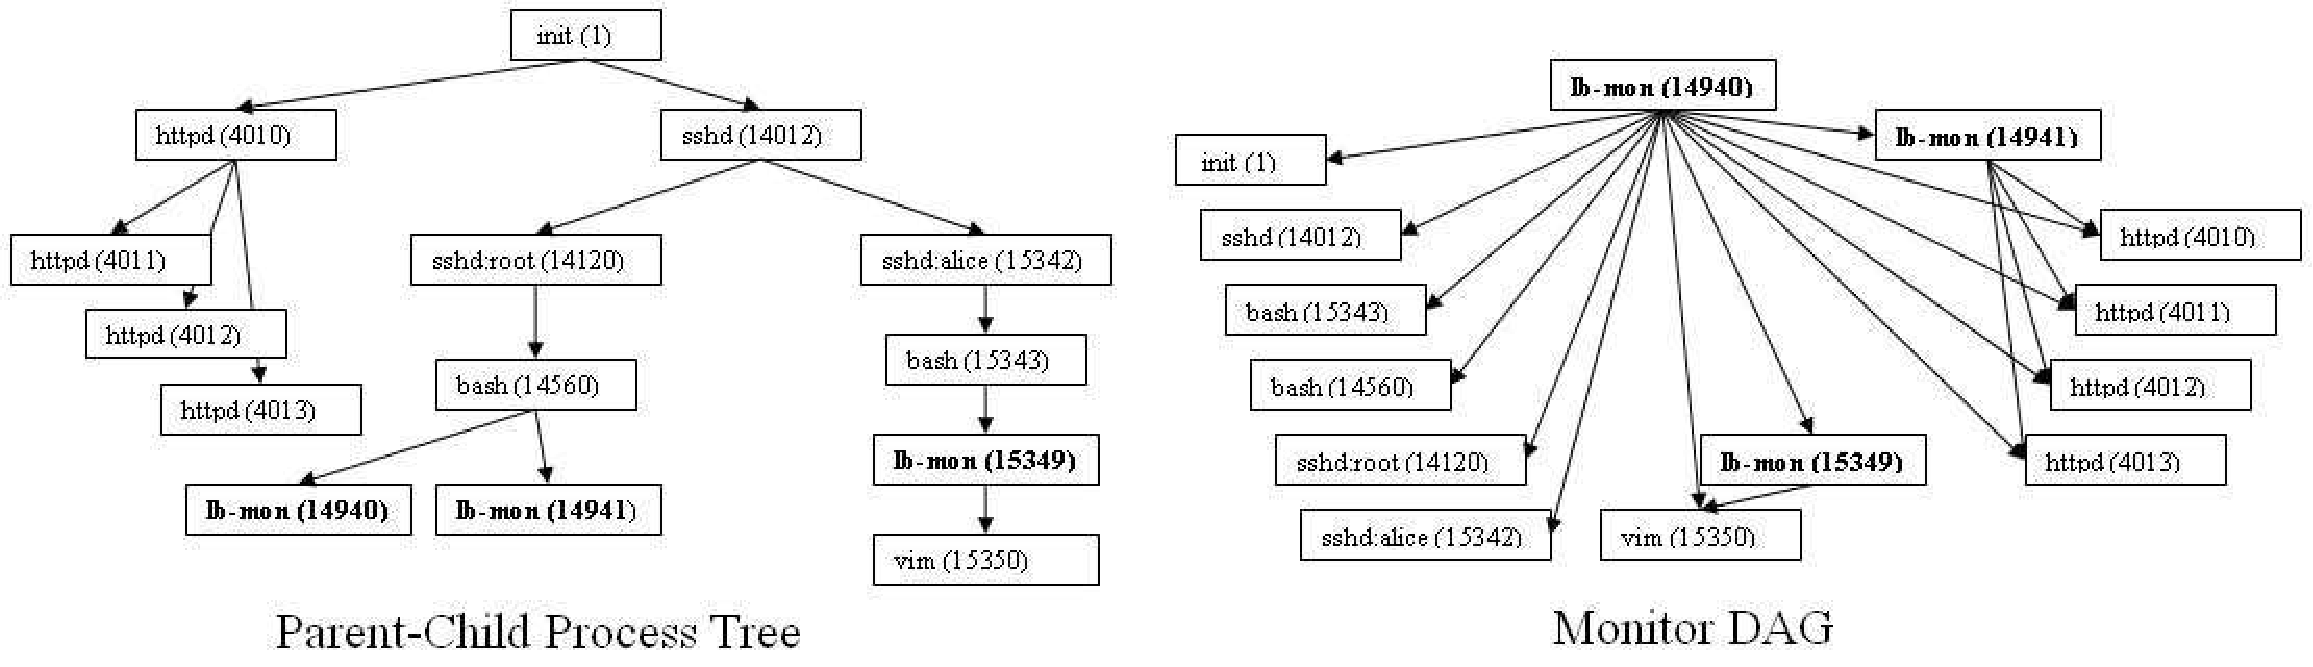
\includegraphics[scale=0.4]{lbox/mon-both}
\caption{A Tree of Cascaded Monitors}
\label{mon-tree}
\end{figure*}


% While a simple example was used, it should be clear that only
% a fairly minimal kernel mechanism which is attached
% to relevant actions and objects is needed.
% The monitor process can pretty much do anything. 
% LAFS \cite{lafs}
% is a logging and auditing file system where accesses not conforming
% to a policy are logged.
% The policy specification
% includes a time interval, userid specification, application
% and operation type. A LAFS-like monitor could easily be written.
% While file events do not specify the application issuing the operation,
% the monitor can reconstruct this from the {\tt execve} events.
% Note that it is harder to use {\tt DTrace} to do this LAFS-style tracing 
% because of its system call orientation. Here we can make use of 
% inheritance in the directory structure. 
% A related but slightly simpler monitor is to audit whether
% the apache web server is used to access any unexpected files.

% In \cite{finke} a monitoring application is described to report when 
% applications tasks did not run as they were supposed to, e.g. due to some
% failure. Again, it is easy to write a monitor which can detect whether
% tasks ran as scheduled.

%% can add application events

\subsection{Using Monitors}

We now give some simple examples of using the framework.
This examples are only meant to exemplify the ease of creating
a customized auditing monitor and are not meant to be full blown applications.

\subsubsection{Testing a possibly untrusted program}

This example checks to see if a process is not stealing your PGP keys.
The monitor process first creates the lbox and then a child process
which executes the program to be audited.

{
\small
\begin{verbatim}
  proc_spec = lbox_CHILDOF(getpid());
  lbox_addevent_file(event_spec,
    "/home/alice/.gnupg/secring.gpg",
    SELF, F_R, I_ALL);
  // .... create the lbox
  if (fork()) {
          // .... do the event processing
  } else execl(....);
\end{verbatim}
}

% The process specification is described by all the child processes 
% of the monitor.
% This makes sure there is no race condition between monitor
% creation time and child process execution time.
% Note that the monitor never monitors itself,
% because it will create a monitoring cycle.
% It is automatically removed from the set of monitored processes.


\subsubsection{Monitoring the web server}

In this example, we want to see whether the web server is working correctly.
More precisely, we want to make sure it is only accessing files inside
\code{/var/www}.

The process specification can be described as follows:
{
\small
\begin{verbatim}
  proc_spec = lbox_CHILDOF(apach_master_pid);
\end{verbatim}
}
\noindent
The event specification is an example of
monitoring files {\em outside} some directory.
We first make all files to be monitored, then we make
all files under \code{/var/www} {\em not} to be monitored.
Note that the order of the two specifications is not important.
{
\small
\begin{verbatim}
  lbox_add_event_file(&event_spec1, "/",
    SELF|SUBDIRECTORIES, F_R|F_W, I_ALL);
  lbox_add_event_file(&event_spec2,
    "/var/www", IGNORE, F_R|F_W, I_ALL);
\end{verbatim}
}
% In the first event specification,
% we make all files to be monitored by issuing the root
% directory and its subdirectory to be monitored.
% In the second event specification,
% we get rid of \code{/var/www} by using IGNORE as the
% directory inheritance flag.

\subsubsection{Global Monitoring}

Sometimes you need to monitor all actions on a single process;
and other times you need to monitor a single action on all processes.
In this example, we want to see if any process is sending packets
to the network \code{137.132.0.0/255.255.0.0}.
The process specification is simply, \\
{\small\verb|  proc_spec = lbox_TRUE();|} \\
The event specification is the following network event, \\
{\small\verb|  lbox_net_connect_ipv4(&event_spec,|} \\
{\small\verb|    "137.132.0.0/255.255.0.0");|}

\subsubsection{Other Applications}

LAFS \cite{lafs}
is a logging and auditing file system where accesses not conforming
to a policy are logged.
The policy specification
includes a time interval, userid specification, application
and operation type. A LAFS-like monitor could easily be written.
Note that it is harder to use {\tt dtrace} to do this LAFS-style tracing 
because of its system call orientation. Here we can make use of 
inheritance in the directory structure. 

In \cite{finke} a monitoring application is described to report when 
applications tasks did not run as they were supposed to, e.g. due to some
failure. Again, it is easy to write a monitor which can detect whether
tasks ran as scheduled.

% \subsection{Implementation Issues}
% 
% \subsubsection{The Hooking Mechanism}
% 
% The prototype implementation we have is in Linux on the 2.6 kernel series.
% There are several ways of implementing the monitor mechanism:
% \begin{enumerate}
% \item Making use of the {\tt ptrace()} or {\tt /proc} facility.
% As discussed earlier, this has many problems and does not support
% mandatory or reliable monitoring. A system-call based mechanism
% is also not suitable for our object-based orientation.
% \item Some other in-kernel system call interposition method.
% This can suffer from TOCTOU (time of create time of use) problems.
% For example, if we are monitoring the {\tt write()} system call,
% a process can change the actual file which the file descriptor points to
% between the time when the file descriptor is looked up and 
% the actual file descriptor is used.
% This would lead either to missing an event (unreliability) or
% reporting an incorrect event (the wrong file).
% As before, it also does not suit our object-based orientation.
% \item Using the LSM hooks in Linux 2.6.
% We currently use this approach in our prototype which has a good
% match with kernel objects. Its also much simpler as LSM hooks are
% mostly in the right places.
% It guarantees mandatory monitoring, and does not suffer from TOCTOU.
% However, it does not cover every possible system calls.
% As the present prototype focuses initially on events on files,
% this is sufficient but it does mean that a full solution cannot be
% just a module.
% \end{enumerate}
% 
% \subsubsection{Matching The File Specification}
% 
% Matching file event specifications, requires the 
% deeper matching file event specification to take precedence.
% To achieve this, the algorithm for checking of a file access is as follows.
% \begin{enumerate}
% \item If the current file is marked SELF, report it (generate event), done.
% \item If the current file is marked SUBDIRECTORIES, report it (generate event), done.
% \item If the current file is marked IGNORE (neither SELF nor SUBDIRECTORIES), ignore it,
% done.
% \item If it is the root directory, ignore it, done.
% \item Set parent directory as current file.
% \item Goto 2.
% \end{enumerate}
% 
% Suppose we have the following two file event specifications
% from the previous example:
% \begin{enumerate}
% \item {\tt (/, SELF|SUBDIRECTORIES, R|W)}
% \item {\tt (/var/www, IGNORE, R|W)}
% \end{enumerate}
% For the file /var/www/a/b/c, the checking is stopped
% at {\tt /var/www} at the third step.
% For the file /etc/passwd, the checking is stopped
% at {\tt /} at the second step.
% 
% To do the upward directory traversal, we make use of the
% {\tt dentry} kernel structure.
% The upward directory traversal is fast, because in Linux,
% during the path resolving phase, all the parent {\tt dentry}
% nodes are stored in the {\tt dcache}.
% 
% \subsubsection{Performance Tuning Methods}
% 
% To reduce the overhead of of task switching caused by our auditing system,
% we introduce an event buffer so that the monitored process 
% can continue its execution even if it generates a auditing event.
% Timeouts and events with a flushing property
% are used to ensure that the monitor can still get events
% even if the buffer is not full and the monitor can choose
% a tradeoff between efficiency and timeliness.
% 
% When a system call takes place, we first check whether the process is being
% monitored.
% This check only requires a few instructions.
% Thus there is very little impact on non-monitored processes.
% For monitored processes, the monitor can also be found efficiently.
% Thus there is very little impact on a process as long as
% the number of logboxes which contains the process is not too large.
% 
% The time required for checking whether the event should be logged
% varies with different types of events.
% A direct operation involving the file is very efficient.
% If there is any file event which involves inheritance,
% we need to trace the file all the way up to the marked file 
% or the root directory.
% Since all the information of parent files is in the dentry cache,
% the directory traversal should be fast.
% Other kinds of objects can be equally fast, for example,
% with a socket connection event, we only need to do the netmask test.

\subsection{Experimental Evaluation}

Our prototype Linux implementation makes use of LSM \cite{lsm} and
version 2.6.10 of the kernel,
and thus is convenient to install
as it consists of loadable kernel modules.
The interface to the kernel is done through \code{ioctl} to a pseudo filesystem
in \code{/proc/lbox}.
The lbox API library in Section \ref{sec:framework} 
gives a more convenient interface that using \code{ioctl} system calls.
Due to lack of space, we do not go into further details
of the kernel implementation.
The PC used here is a Pentium IV 3.0GHz PC with 1G memory.

We want to demonstrate that the framework and prototype system leads
to rather efficient monitoring. Although our prototype is not yet
fully optimized, the results do show that the overheads of monitoring
can be very low.

We first use a simple micro-benchmark which gives an indication
of worse case overheads.
The program performs 1000000 open(2) and close(2) calls with
a monitor watching for the file access.
We compare the auditing framework in each of the following scenarios:
\begin{enumerate}

\item {\em clean kernel}:
A clean stock kernel.

\item {\em proc miss}:
The lbox module is loaded in the kernel but no monitors are present.
% However, no monitor is monitoring the busy-open process.

\item {\em file miss 1/2}:
A monitor is monitoring the file open but on a different file specification.
Thus no event is generated.
We compare two scenarios.
{\em File miss 1}, uses a directory specification without the
SUBDIRECTORIES property, thus no directory traversal is needed.
{\em File miss 2} has a file specification which is some non-matching
directory with the SUBDIRECTORIES set.
This requires traversing up ancestor directories up to the root.
% check whether the event can match the directory specification.
% The difference between the two scenarios is whether directory traversal
% is needed. 
% SUBDIRECTORIES flag set, whereas in {\em file miss 2}, there is a file spec
% which has SUBDIRECTORIES flag set, thus we need to traverse all the way up to
% the root directory to make sure that the action does not match the file spec.

\item {\em 0 dir level}:
The monitor is monitoring a regular file.
The benchmark is accessing the same regular file.

\item {\em 1/2 dir levels}:
The monitor is monitoring a directory which is 1 or 2 levels deep containing
the which is being used.
For example, the monitor uses the file specification
\code{/1} with SUBDIRECTORIES set.
The 2 dir level benchmark opens the file \code{/1/2/foo}.
This test investigates the time for directory traversal..

\item {\em no buff}:
The file event is synchronous which means 1000000 context switches
to the monitor are needed.
The benchmark process suspends until the monitor
has read the event

\item {\em ptrace}:
The comparison is with \code{strace} which uses the traditional
\code{ptrace} mechanism in Linux.

\end{enumerate}

\begin{table}
\small
%\begin{center}
\centering
\begin{tabular}{ | l || c | c | c | }
\hline
scenario & real & user & sys \\
\hline \hline
clean kernel & \begin{math} 1.99\pm0.01 \end{math} & \begin{math} 0.21\pm0.01 \end{math} & \begin{math} 1.77\pm0.02 \end{math} \\
proc miss & \begin{math} 2.04\pm0.02 \end{math} & \begin{math} 0.21\pm0.01 \end{math} & \begin{math} 1.82\pm0.03 \end{math} \\
file miss 1 & \begin{math} 2.17\pm0.01 \end{math} & \begin{math} 0.22\pm0.01 \end{math} & \begin{math} 1.95\pm0.02 \end{math} \\
file miss 2 & \begin{math} 2.27\pm0.01 \end{math} & \begin{math} 0.22\pm0.01 \end{math} & \begin{math} 2.04\pm0.02 \end{math} \\
1 dir level & \begin{math} 2.29\pm0.01 \end{math} & \begin{math} 0.21\pm0.01 \end{math} & \begin{math} 2.03\pm0.02 \end{math} \\
2 dir levels & \begin{math} 2.52\pm0.01 \end{math} & \begin{math} 0.21\pm0.01 \end{math} & \begin{math} 2.23\pm0.03 \end{math} \\
3 dir levels & \begin{math} 2.56\pm0.01 \end{math} & \begin{math} 0.20\pm0.02 \end{math} & \begin{math} 2.31\pm0.02 \end{math} \\
no buff & \begin{math} 8.70\pm0.04 \end{math} & \begin{math} 0.99\pm0.08 \end{math} & \begin{math} 4.57\pm0.16 \end{math} \\
ptrace & \begin{math} 59.04\pm0.15 \end{math} & \begin{math} 12.90\pm0.32 \end{math} & \begin{math} 46.11\pm0.39 \end{math} \\
\hline
\end{tabular}
%\end{center}
\caption{Open micro-benchmark}
\label{tab-open}
\end{table}

The open micro-benchmark results are given in Table \ref{tab-open}
with all times in seconds. The average and standard deviation
is given over 10 runs.
As the timings are only measured with the Unix user/system and real-time
mechanism, they are only approximate and are meant
to give an indication of the overheads of monitoring
under the different scenarios.

The kernel inspection implementation (proc miss) has negligible overhead
($\sim 2\%$) over the clean kernel.
The {\em file miss 2} test has ($\sim 14\%$) overhead, this is because that
the system needs to travel to the root directory to make sure the file is
not monitored.
{\em file miss 1} has a smaller overhead ($\sim 9\%$) because directory
traversal is not needed.
When monitoring is synchronous, so events are not buffered (no buff),
overhead jumps substantially to $337\%$.
It is interesting to note that this is still much smaller than {\tt ptrace}
which has $2866\%$ overhead or about seven times slower than the
no buffering case.
Using asynchronous events with buffering (0 dir level) 
drops the overhead to $15\%$.

One point of comparison with other systems on Linux would be with
Systrace \cite{systrace}. 
A pure comparison is not valid since in our system any event
which must be monitored is eventually passed to the monitor.
Systrace on the other as it does access control first can choose between a
kernel-level policy or the user-level policy daemon. 
The kernel-level policy should entail less work for Systrace
simply because the decision is handled only within the kernel, while
the user-level policy is more expensive simply due to the increased
number of context switches.
The objectives of the two systems are also different.
With those caveats in mind, the Systrace open micro-benchmark shows a
$6.25\%$ overhead over no monitoring.
Our overhead for {\em file miss 1} is a little more at $9\%$.
This makes sense since for auditing,
an event has to cross in two directions: first inwards when it is recorded; 
and later back to user-space when it is sent to the monitor.
Our implementation is not yet optimized and we expect also to be
able to reduce the overheads further.

Our directory file specifications can be compared against the 
pathname normalization of Systrace.
The ``0-2 dir levels'' scenario shows that the overhead of an inherited
file specification is small, the initial overhead of checking a directory is
reasonable at $26\%$ and then a rather small overhead for the next component.
The Systrace results show that each directory
component in their specification adds about $1665\%$ additional overhead
over the original {\tt open()} system call.
This is because of the filename normalization done in user-space which
is significantly more expensive.

\begin{table}
\small
%\begin{center}
\centering
\begin{tabular}{|l||c|c|c|}
\hline
scenario & real & user & sys \\
\hline \hline
direct run & \begin{math} 3.84\pm0.01 \end{math} & \begin{math} 1.04\pm0.01 \end{math} & \begin{math} 2.80\pm0.01 \end{math} \\
\hline
truss & \begin{math} 100.32\pm0.85 \end{math} & \begin{math} 10.12\pm0.05 \end{math} & \begin{math} 56.71\pm0.80 \end{math} \\
\hline
DTrace\footnotemark & \begin{math} 8.41\pm0.02 \end{math} & \begin{math} 1.08\pm0.01 \end{math} & \begin{math} 7.33\pm0.01 \end{math} \\
\hline
\end{tabular}
%\end{center}
\caption{Open micro-benchmark on Solaris 10}
% (SunOS 5.10 i386)}
\label{tab-sol}
\end{table}

\footnotetext[2]{The D program is ``syscall::open:entry \{ @[execname]=count(); \}''}

Table \ref{tab-sol} shows the
test on Solaris for the same hardware with the same benchmark program. 
While the baseline for Solaris is slower than Linux, it is reasonable
to make relative comparisons.
\code{Truss} which uses the \code{proc} adds $2510\%$ overhead 
to the \code{open()} system call and DTrace is significantly more efficient
with $119\%$ overhead.
The use of \code{proc} allows only the \code{open()} system call to
be traced rather than all system calls. Even so, we see that the overhead
is considerably higher than in Linux where \code{ptrace} traces every
system call.
In the DTrace test, we have allowed DTrace more advantage 
as the D program does not return any information to user space, 
whereas in our system, all
the relevant {\tt open()}'s are being
returned to the user space monitor.
The absolute running time in the DTrace test is 3.67 times 
of that in our system.
The overhead added to the original system call in DTrace is 7.9 times of
that in our system.
This is slightly surprising since DTrace uses dynamic instrumentation
(which is hardware dependent) while we use a simpler static instrumentation
which is more expensive but portable.
We suspect it is partly a case of the Linux kernel having less overhead
than Solaris.

% Since the open micro-benchmark reuses the same file over and over again,
% the open itself becomes quite fast in Linux. 
% We use another micro-benchmark on socket
% operations to show the effect of a more expensive system call.
% The benchmark creates a TCP socket and connects to a local port.
% This is repeated for 4000 times and the results are in Table \ref{tab-connect}.
% We can see that in an expensive system call, the overhead is not noticeable.

% \begin{table}
% %\begin{center}
% \centering
% \begin{tabular}{ | l || c | c | c | }
% \hline
% environment & real & user & sys \\
% \hline\hline
% clean kernel & \begin{math} 0.27\pm0.01 \end{math} & \begin{math} 0.01\pm0.01 \end{math} & \begin{math} 0.20\pm0.01 \end{math} \\
% \hline
% monitored & \begin{math} 0.28\pm0.01 \end{math} & \begin{math} 0.01\pm0.01 \end{math} & \begin{math} 0.20\pm0.01 \end{math} \\
% \hline
% \end{tabular}
% %\end{center}
% \caption{Connect micro-benchmark}
% \label{tab-connect}
% \end{table}

\begin{table*}[ht]
\centering
\begin{tabular}{ | l || c | c | c | }
\hline
 & web server (request/sec) & make bash (sec) & install mozilla (sec) \\
\hline\hline
Linux clean & \begin{math} 8903.1\pm21.8 \end{math} & \begin{math} 34.3\pm0.2 \end{math} & \begin{math} 1.8\pm0.1 \end{math} \\
\hline
lbox no I/O, file miss & \begin{math} 8773.1\pm19.4 (1.5\%) \end{math} & \begin{math} 34.4\pm0.2 (0.17\%) \end{math} & \begin{math} 1.8\pm0.0 (0\%) \end{math} \\
\hline
lbox no I/O, file hit & \begin{math} 8762.0\pm25.6 (1.6\%) \end{math} & \begin{math} 34.4\pm0.2 (0.17\%) \end{math} & \begin{math} 1.8\pm0.0 (0.56\%) \end{math} \\
\hline
lbox with I/O & \begin{math} 8728.9\pm18.4 (2.0\%) \end{math} & \begin{math} 34.4\pm0.2 (0.29\%) \end{math} & \begin{math} 1.7\pm0.1 (3.9\%) \end{math} \\
\hline
strace no I/O & \begin{math} 3577.6\pm8.5 (148.9\%) \end{math} & \begin{math} 39.6\pm0.1 (15.3\%) \end{math} & \begin{math} 2.2\pm0.1 (21.1\%) \end{math} \\
\hline
strace with I/O & \begin{math} 1981.4\pm6.9 (349.3\%) \end{math} & \begin{math} 100.7\pm0.1 (293.2\%) \end{math} & \begin{math} 23.2\pm0.1 (1189.4\%) \end{math} \\
\hline\hline
Solaris clean & \begin{math} 6889.1\pm42.6 \end{math} & \begin{math} 43.8\pm0.1 \end{math} & \begin{math} 1.6\pm0.1 \end{math} \\
\hline
DTrace no I/O & \begin{math} 6776.2\pm53.6 (1.7\%) \end{math} & \begin{math} 44.4\pm0.1 (1.4\%) \end{math} & \begin{math} 1.6\pm0.1 (0\%) \end{math} \\
\hline
DTrace with I/O & \begin{math} 6326.9\pm52.4 (8.9\%) \end{math} & \begin{math} 44.5\pm0.0 (1.6\%) \end{math} & \begin{math} 1.6\pm0.0 (0.6\%) \end{math} \\
\hline
truss no I/O & \begin{math} 1382.0\pm2.0 (398.5\%) \end{math} & \begin{math} 70.9\pm0.0 (61.8\%) \end{math} & \begin{math} 7.7\pm0.0 (372.2\%) \end{math} \\
\hline
truss with I/O & \begin{math} 1126.7\pm4.4 (511.5\%) \end{math} & \begin{math} 74.6\pm1.5 (70.2\%) \end{math} & \begin{math} 13.4\pm0.13 (724.7\%) \end{math} \\
\hline
\end{tabular}
\caption{Macro-benchmarks}
\label{tab-macro}
\end{table*}

The \code{open} micro-benchmark gives a measure of worst-case overhead
since the file is totally cached in memory and in that case, the Linux
\code{open} code is heavily optimized.
It is also useful to look at applications (macro-benchmarks
which do more than just system calls) which may have moderate to
moderately heavy system call usage. Obviously, there is little point
benchmarking CPU bound applications which only have low system call use.
In the macro-benchmarks, we also look at the cost of monitoring 
I/O (reading and writing), this is meant to simulate a monitor which might
want to examine precisely what an application has done.
We have chosen three application benchmarks which are realistic applications
\begin{itemize}
\item apache web server: this is chosen because web server performance
is important.
For apache, we measure the average number of requests served per second
using the apache \code{ab} benchmark and I/O monitoring is for
the http requests (reading) and http responses (writing).

\item \code{make bash}: this builds the bash shell.

\item install mozilla: this installs mozilla. The
Linux and Solaris differ. The Linux one has a custom
install program while the Solaris version is simply untar.
This means the results are not comparable except in a relative
to each operating system alone.
\end{itemize}

The last two benchmarks, bash and mozilla,
have also been chosen because these applications
have been used in Alcatraz.
For I/O monitoring, we have monitored all the I/O from the application.
The results given in Table \ref{tab-macro}. 
The results for \code{strace} and \code{truss} are only meant to illustrate
the additional overhead of I/O since both programs do reprocess the data
and thus do have additional overhead but 
serves to bound the cost of \code{ptrace} and \code{proc}.
We see that in all cases, lbox monitoring has very low overheads, below
$2\%$ without I/O and less than $4\%$ with complete I/O monitoring of the
applications.
The mozilla install cannot be directly compared since the actual install
is different.
Even though these are macro-benchmarks, 
overhead for \code{ptrace} without I/O is significant, at least $15\%$.
With I/O monitoring, the overhead shoots up.
Alcatraz \cite{alcatraz} which uses \code{ptrace} has rather
high overheads for their system call interception, $43\%$ for a \code{make}
and $79\%$ for \code{mozilla}. Their isolation overhead which is a measure
of write I/O adds a further $20\%$. Our overheads are much smaller ($< 4\%$)
but we don't do isolation.

It is a little surprising that our user-level auditing framework
can out perform DTrace which is an in-kernel tracing mechanism.
This is very encouraging and furthermore, 
we believe we can still optimize our prototype.

\subsection{Conclusion}

We show a user-level auditing framework suitable for general purpose
auditing and security monitoring. 
We achieve transparent auditing
at a fine-grained level of applications while providing guarantees
on the security of the auditing process. We are careful to avoid problems
with privilege escalation and access to information beyong the user's
privileges. Furthermore, we avoid problems associated with denial of
service which can be caused by self-referential monitoring or tracing.

As our monitors are user-level, the auditing is expressed in terms
of operations on operating system objects and resources. This makes it
easy to write a custom monitor since the semantics is close to that
of user code rather than having to understand kernel internals.

A user-level monitor is desirable given it is more safe than an in-kernel one.
The question is whether a user-level monitor is sufficiently efficient. 
Our framework is designed so that the cost of monitoring
is commensurate with the amount of events and information needed.
Our experiments are very encouraging 
showing that the overhead is comparable to in-kernel 
mechanisms such as DTrace.

Future work includes further system optimizations to make the framework
even more scalable and efficient. We would like to increase the
expressivity of the in-kernel mechanisms without incurring more cost
and also avoiding executing monitor code in the kernel.

% \begin{thebibliography}{99}
% 
% \bibitem{dtrace-paper}
% Bryan M. Cantrill, Michael W. Shapiro and Adam H. Leventhal,
% ``Dynamic Instrumentation of Production Systems'',
% Usenix, 2004.
% 
% \bibitem{finke}
% J. Finke,
% ``Process Monitor: Detecting Events That Didn't Happen'',
% Usenix LISA, 2002.
% 
% \bibitem{garfinkel}
% T. Garfinkel,
% ``Traps and Pitfalls: Practical Problems in System Call 
% Interposition Based Security Tools'',
% Network and Distributed Systems Security Symp,
% 2003.
% 
% \bibitem{janus}
% I. Goldberg, D. Wagner, R. Thomas, and E. Brewer,
% ``A Secure Environment for Untrusted Helper Applications'',
% Usenix Security, 1996.
% 
% \bibitem{alcatraz}
% Z. Liang, V.N. Venkatakrishnan, and R. Sekar, 
% ``Isolated Program Execution: An Application
% Transparent Approach for Executing Untrusted Programs'',
% ACSAC, 2003.
% 
% \bibitem{systrace}
% N. Provos,
% ``Improving Host Security with System Call Policies'',
% Usenix Security, 2003.
% 
% \bibitem{solaris-sec-svc}
% Sun Microsystems,
% ``System Administration Guide: Security Services'',
% part IV: Auditing and Device Management.
% 
% % \bibitem{dtrace-man}
% % Sun Microsystems,
% % ``Solaris Dynamic Tracing Guide''.
% 
% \bibitem{lafs}
% C. Wee,
% ``LAFS: A Logging and Auditing File System'',
% Annual Computer Security Applications Conf,
% 231--240, 1995.
% 
% \bibitem{lsm}
% C. Wright, C. Cowan, S. Smalley, J. Morris, and G. Kroah-Hartman,
% ``Linux Security Modules: General Security Support for the Linux Kernel'',
% Usenix Security, 2002.
% 
% \bibitem{dprobes}
% Dynamic Probes,
% {\small\tt http://dprobes.sourceforge.net/}
% 
% \end{thebibliography}
% 
% \end{document}

\clearpage
\section{WinResMon: a Resource Usage Logging Framework for Windows}

%winresmon\cite{ramnath2006winresmon} for windows

\subsection{Introduction}

The tasks of software maintenance and configuration require a precise
understanding of system resources, the individual requirements of each piece
of software, and interdependencies between every software program on the
system.  We use the term {\em software maintenance} to describe the system
administration task of ensuring that software on a system is configured and
maintained correctly over time.  Examples of software dependencies include:

\begin{itemize}
\item file sharing: including dynamic libraries and external data storage.
\item sharing of software configurations: usually in the form of registry keys
in Microsoft Windows.
\item interprocess communication and synchronization.
\end{itemize}

Although software maintenance tasks might seem conceptually trivial, they can
be time consuming and difficult, especially in large or complex environments.
System administrators often rely on documentation and on-line information such
as FAQs or forums, but such information is often incomplete.

In various distributions of Linux, software dependency issues are partly
addressed by the use of a package manager.  The Red Hat Package Manager (RPM)
\cite{rpm}, for example, records the currently installed packages and the
files required and provided by these packages in a centralized database.  RPM
checks dependencies before removing a package to ensure that files required by
other installed packages are not removed.  Similar checks are done to prevent
installing a package which contains files that conflicts with other existing
packages.

In Microsoft Windows, however, software installation can be complex, and the
exact dependencies between different software programs might not be clear.
The confusion is further compounded by many implicit software
interdependencies, e.g. registry keys which are part of shared software
configurations.  As a result, it is difficult to know whether to remove a file
when uninstalling an application.  File removal might lead to problems with
another piece software or might create security vulnerabilities.  

When installing two or more programs that share files, one program may cease to
function correctly because the installation of the second blindly overwrote 
shared libraries (DLL files).  There is also the question of when to perform a
major software upgrade.  System administrators may delay upgrading
for fear of breaking existing software; yet such a choice has its own risks.

This paper focuses on the problem of software
maintenance in Microsoft Windows NT-based operating systems (Microsoft Windows
XP, Microsoft Windows 2000, Microsoft Windows 2003).\footnote{ While an
appropriate version of a tool similar to WinResMon could also be of use in UNIX,
its value is much greater in a Microsoft Windows environment.  } We present {\em WinResMon},
a discovery and system debugging tool for
determining a program's resource usage as well as the resource usage
interactions between multiple programs.


\subsection{Motivation and Applications}

We believe that the key to solving the software maintenance problem is to
understand the life cycle of the system and programs therein.  We also wish
to empower ordinary users, removing the requirement of knowing every minutiae
of Microsoft Windows.  Although WinResMon is not tailored specially for system
security, it can also be utilized as a security auditing tool.

We designed WinResMon to act as both an infrastructure or framework
and a system utility.  
As a framework, it is extensible, and one can therefore add
new functionality and build customized tools.  As a tool, it comes with
pre-built modules to answer typical questions about resource usage and
dependencies.

When used as a debugger, WinResMon investigates the current system state,
i.e. which program uses which registry keys, and determines how the system has
arrived at that state.  WinResMon accomplishes this by recording information
about the evolution of system software dependencies and resource usage over
time.  To solve general problems in software maintenance, WinResMon monitors:
files, the registry, and interprocess communication and synchronization.
However, it is not feasible to continuously and permanently record all changes
to the system since the required space would be prohibitive.  
WinResMon employs
a reasonable compromise by maintaining detailed usage records 
over the current time period and a
subset of information that can be maintained over the lifetime 
of all software in the system.

We illustrate the software maintenance problem with some simple examples.  One
attack vector for spyware is to register itself as a start-up program, thereby
hiding itself from the end user.  Also consider a music player which may
require some sound decoding libraries.  This application only functions
correctly with certain versions of the libraries.  Thus, replacing a library
can lead to software failure.  Various pieces of software may also conflict,
e.g.  two mail transfer agents (MTAs) usually do not co-exist.

Some common system administration questions and tasks which WinResMon 
can assist with include:

\begin{enumerate}

\item Can we safely remove a particular DLL file?

Some applications provide shared libraries (DLL files) for use with other
applications.  When the system administrator uninstalls an application, she
can also choose to remove the DLLs.  Removing a DLL can cause other programs
which still use it to malfunction.  On the other hand, blindly retaining all
DLLs will cause the system to keep growing and may create security
vulnerabilities.  The system administrator generally lacks adequate
information to determine whether another program uses a shared
library. WinResMon can be used to record the utilization of each DLL so that the
system administrator can determine which programs use which DLLs.

\item Why does a program need administrator privilege to run?

Running programs with administrator privilege is discouraged because malware
such as viruses/spyware or poorly written applications can damage the system.
However, some programs may need to run as the administrator without an obvious
reason.  WinResMon can detect whether a program needs administrator access.  The
idea is to understand the reasons for elevated privileges and configure the
system to limit the use of privileges.  If it finds applications that require
certain administrator privileges to function correctly, the system
administrator can set up a policy that restricts the administrator privileges
to the needed resources (files, registry keys, etc).  
We remark that this approach can be contrasted with confinement systems
such as systrace \cite{systrace} in Unix.
WinResMon is an auditing tool, it does not confine system calls, but
provides useful input for system administrators to create policies 
on resource access which can then be used to limit privileges.

\item Monitoring sensitive registry locations to detect spyware.

Managing the Microsoft Windows registry is difficult due to its complexity.
Spyware often takes advantage of this complexity to bury itself in the
registry, making it difficult for the user to remove it completely.  In
\cite{asep}, the authors have listed the most common entry points for spyware
to enter a Windows NT system.  The following are some of the configuration
settings WinResMon can monitor:

\begin{itemize}

\item {\em Autostarts}: monitor which programs load on startup.
\item {\em Internet explorer hooks}: track hooks which define
the default search page, toolbars and browser helper objects (BHO), etc.
\item  {\em Winlogon}: look for applications that hook into system
resources.
\item  {\em Services}: monitor services such as automatic startup services
(e.g. task scheduler) or drivers which are installed as services.
\item {\em DLL injection}: monitor DLL injection attacks (any application
that uses {\small\tt user32.dll} can be hijacked by having a DLL injected into its
process space).
\item {\em File associations}: monitor the registration of file extensions
with applications.  For example, {\small\tt .DOC} is registered to Microsoft Word.

\end{itemize}
\end{enumerate}


\subsection{System Design}

The WinResMon system infrastructure shown in Figure~\ref{usp} consists of the
following components: logger, archiver, query API, and user-log API.  
The logger generates
resource-access traces which are later used by the analyzer.  The archiver
performs log compaction/summarization of old traces.
Query and user-log API provide the interface to the trace database.

\begin{figure*}
\centering
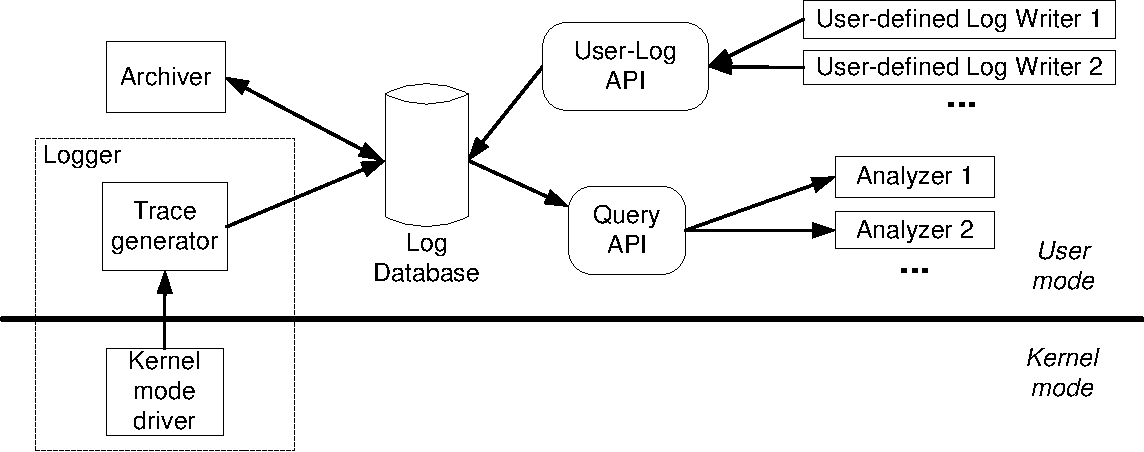
\includegraphics[scale=0.6]{winresmon/usp}
\caption{WinResMon overall system architecture}
\label{usp}
\end{figure*}


\subsubsection{The Logger}

The logger consists of a system call (syscall) interceptor and a trace
generator module.  The syscall interceptor is an in-kernel driver which
monitors system calls made by each process and sends the monitored event
information to the trace generator.  The trace generator is a user-space
service (daemon) which collects event information sent from the syscall
interceptor and generates resource access traces.  Ideally, the logger is
meant to run {\em all the time} so as to record the entire life cycle of how
resources are used by software.\footnote{ One might only run the
logger at select times instead, but this means WinResMon could miss critical information. }

A log trace file consists of a list of records, each representing 
an access operation on one of the following types of resource:

\begin{enumerate}
\item {\em File}: covering both directories and regular files
\item {\em Registry}
\item {\em Process}: mainly to record process creation
\item {\em Synchronization objects}: which records information on
inter-process synchronization mechanisms provided by Microsoft Windows (mutex,
semaphore, event and waitable timer)
\item {\em IPC}: including named pipes and mailslots.
\end{enumerate}

In addition to these five basic resource types, WinResMon also captures {\it
system event} information such as: process termination, system boot and
shutdown, user login and logout.  
Moreover, it also provides a user-log API
(described in Section~\ref{sect:custlog}) for users or applications to insert
user/application-defined milestone events.  One potential usage of custom
events is to demarcate and distinguish the software installation and
uninstallation portions of the log.

A record entry contains common information and specific information
relevant to that record type.
The common information consists of: {\em record-type}, 
{\em time}, {\em process-id}, and the {\em error-code} 
(in the case of failure).  
The specific information recorded by different record types are:

\begin{enumerate}
\item {\bf File:}
\begin{itemize}
\item absolute path of the file
\item file operation: {\em open}, {\em read}, {\em write}, {\em delete}
or {\em move}
\item operation-specific information. For open: the access flags.  For read
and write: the number of bytes read or written.  For move: the new path.
\end{itemize}

\item {\bf Registry:}
\begin{itemize}
\item absolute path of the registry key
\item operation:  {\em open-key}, {\em query-value}, {\em set-value}, or {\em
delete-key}
\item operation specific information.  For {\em open-key}: the access
flags. For {\em query-value} and {\em set-value}: the type, size, and value of
the registry key.
\end{itemize}

Due to the importance of the registry in software maintenance, WinResMon logs the
actual data changes made to the registry; whereas for file I/O, it is not
practical to record the data.

\item {\bf Process:}
\begin{itemize}
\item absolute path of the executable corresponding to the newly created
process
\item command line arguments
\item process id of the newly created process.
\end{itemize}

\item {\bf Synchronization objects:}
\begin{itemize}
\item type of the object:  {\em mutex}, {\em semaphore}, {\em event}, or
{\em waitable-timer}
\item name of the object
\item operation: {\em create}, {\em open}, or {\em delete}.
\end{itemize}

We are interested only in objects which have names in the system-wide
namespace, because anonymous and process-wide named objects will not interfere
with other programs, thus they are unrelated to software dependencies.

\item {\bf IPC:}
\begin{itemize}
\item type of the IPC: {\em named-pipe}, or {\em mailslot}
\item name of the IPC
\item operation: {\em create}, {\em open}, {\em delete}, {\em send}, or {\em
receive}. 
\end{itemize}

WinResMon records the synchronization objects and IPC operations listed above
since they involve global (system-wide) namespace which could
be used by different programs to interact with each other.
One can use WinResMon to uncover the causes of 
the following problems:

\begin{enumerate}

\item If process $A$ has created a semaphore $s$, and process $B$, which
is unaware of the existence of $A$, is trying to create a semaphore with the
same name $s$, $B$'s operation will fail.

\item If process $A$ fails to run correctly and semaphore $s$ is not
created, then process $B$, assuming the existence of $A$, will fail trying to
use $s$.
\end{enumerate}

\item {\bf System event:}
\begin{itemize}
\item system event type: {\em process-termination}, {\em boot}, {\em shutdown},
{\em user-login}, or {\em logout}
\item any event specific information: path of the executable of the process in
the case of process termination, user name in the case of user login/logout,
etc. 
\end{itemize}

\item {\bf User defined event:}
\begin{itemize}
\item the path of the executable of the process generating the event 
\item a binary string describing the event. 
\end{itemize}

\end{enumerate}

Not all operations need to be logged into the database as some resources are
not significant to record, e.g.  the temporary directory, {\tt
C:$\backslash$temp}.  A filter can therefore be used in the logger to prevent
logging resource access of no interest to the system administrator.


\subsubsection{The Log database}

The log database consists of a number of log files and one
distinguished {\it active log} to which the logger 
records current resource access activity.
To maintain reasonable log file sizes, WinResMon performs a ``log switch'' 
to create a new active log for recording subsequent entries.  The old
log files are then subject to the log compaction/summarization process by the
archiver.  Any of the following conditions can trigger a log switch: \\

\begin{itemize}
\item The size of the current log file reaches the specified {\tt
Max\_log\_size}. \\
\item The number of entries in the current log file reaches
{\tt Max\_log\_entries}. \\
\item The user manually initiates a log switch process.
\end{itemize}


\subsubsection{Archiving Old Traces}

As WinResMon logs system activities over a long period of time, the trace
becomes very large. If old traces are discarded, some early yet potentially valuable information,
such as identifying which program first created a file, is lost. An example of important information is
identifying which program first created a file.  Since it is necessary
to eventually prune some information to avoid excessively large log files,
WinResMon summarizes old trace files into a ``{\em compacted trace database}".
This maintains a balance between compactness and the ability to answer
important questions about system resource access.

There are two main issues in performing trace compaction, determining when to
initiate the compaction and how to perform compaction on old trace entries.
WinResMon uses a module called the archiver which runs based on a specified 
{\tt Archive\_interval\_check} time interval.  Upon activation, the archiver
compacts previously uncompacted entries which are older than the specified 
{\tt Old\_log\_age}.  
WinResMon employs the following strategies in performing the compaction:

\noindent
{\bf 1. Log entry summarization/aggregation}

WinResMon can summarize multiple entries with similar information to produce an
aggregated entry in the compacted trace database.  It applies the following
policies on various resource types:

\begin{itemize}

\item {\bf File:} multiple read or write operations on the same file are
summarized by recording the time of the first and last operations and the
total number of time the operations were done.

\item {\bf Registry:} multiple query-value operations on the same registry key
are aggregated.  Multiple set-value on a key are aggregated only if the values
written are identical.

\item {\bf IPC:} send and receive operations of one IPC object are aggregated
by recording the time of the first and last operations.

\end{itemize}

When matching a query (described later in Section~\ref{sect:queryapi})
on an aggregated entry which records a time interval,
WinResMon considers that the entry satisfies the specified time constraint
if {\it one} of the values matches the constraint.

\noindent
{\bf 2. Selective priority-based entry removal}

One strategy to reduce the old traces involves removing entries deemed to be
of little value for answering future questions. WinResMon implements selective
entry removal strategy based on a user-supplied configuration file.  The
configuration file assigns a priority to log entries.  For example, a log
entry for writing a registry key might be considered more important to keep
than one for reading a registry key.

A fragment of an example configuration is shown in Appendix 2.  This example
uses priority values ranging from 1 (least important) to 5 (most important).
For each resource type, configuration entries are matched in a sequential
order, and mappings are listed from most to least specific.  It is possible to
omit some arguments, i.e. with wildcards.  To simplify the priority
assignment, WinResMon classifies file open operations in Microsoft Windows 
into one of three modes: RO (read-only), RW (read-write) and WO
(write-only/append). The archiver translates the semantics of each operation
from file flags in the raw log entries to the appropriate values for matching
against the configuration.

The existing applications and anticipated usage, together with some general
principles, can be used to derive the priority assignment for the
configuration.  One general principle is that ``transient information,'' such as that
those on synchronization objects and IPC, becomes less relevant after
system shutdown and can be given low priority.  During the removal
process, all log entries with priority lower than the {\tt
Lowest\_priority\_retained} value will be purged.

\noindent
{\bf 3. Auto deletion of old log files}

To maintain reasonable storage usage, WinResMon eventually needs to remove
entries deemed too old.  The log file whose newest entry timestamp exceeds
{\tt Max\_log\_lifetime} is deleted.  If necessary, it is also possible to
additionally provide an API function (in a secure manner) to perform deletion
on selected trace entries based on a specified selection condition.


\subsubsection{A Query API and Analyzer}
\label{sect:queryapi}

We want to support trace analyzers which answer queries solving particular
software maintenance problems.  WinResMon therefore provides a query API which can be 
used to obtain information from the trace database.  
One can view the trace as a database and the provided query API as the query
language by which the analyzers extract relevant information from the
database.

The main query API, analogous to an SQL Select command, is
{\small\tt trace\_select([{\it selection condition}], [{\it field projection}],
[{\it time interval}], [{\it output order}])}, where the caller specifies
the matching condition(s) and fields to return.  The {\small\tt {\it selection
condition}}, specified on string types such as program name and registry key
path, takes the form of a regular expression.  Logical operators can be used
to combine matching conditions.

Continuing the database analogy, the caller uses projection to specify
which fields to return.  For example, suppose one only wants to know the list
of programs accessing a certain file.  In other cases, one wishes to know
all access operations on the file (i.e. the order and access time matter).
In the former, the analyzer only returns a set of program names.  In the
latter, it returns the sequence of all access operations.

We specify {\small\tt {\it time}} in the format below:
\begin{enumerate}
\item ``{\small\tt YYYY-MM-DD hh:mm:ss}'': an explicit timestamp
\item ``{\small\tt -[count][m|h|d]}'': a relative time earlier than the current time
\item ``{\small\tt OLDEST}'': the time of the oldest available entry in the log
\item ``{\small\tt NOW}'': the current time.
\end{enumerate}

The {\small\tt {\it time interval}} is then specified as: ``{\small\tt [{\it start time}] 
TO [{\it end time}]}''.\footnote{ Although an
analyzer can include constraints on log's timestamp as conditions in the
{\small\tt {\it selection condition}}, an explicit time interval specification is
less complex.  }
Some examples of time interval definitions are:

\begin{itemize}
\item ``{\small\tt 2006-01-25 11:47:51 TO 2006-08-21 13:41:16}''
\item ``{\small\tt -1d TO NOW}'' (in the last 24 hours)
\item ``{\small\tt OLDEST TO -8h}'' (everything except the past 8 hours).
\end{itemize}

{\small\tt {\it Output order}} controls the ordering of query results.  It can be
either: {\small\tt FORWARD}, to list the oldest entry first or {\small\tt BACKWARD}, to
show the most recent entry first.  The {\small\tt BACKWARD} option is useful to get
the $k$ most recent operations.

After obtaining the {\small\tt {\it trace\_handle}} from {\small\tt trace\_select()},
one can call {\small\tt trace\_next ({\it trace\_handle})} to retrieve the records
and {\small\tt trace\_close({\it trace\_handle})} to finish retrieval.
Some sample analyzer applications using this query API are described in
Section~\ref{sect:sample}.


\subsubsection{The User-Log API}
\label{sect:custlog}

The user-log API lets applications add their own entries into the log
database.  As applications are not allowed to write directly to the log file,
custom events are generated using an {\small\tt ioctl} interface to the kernel
driver.  One use of user-entries includes marking events related to software
installation, making it easier to determine what files and registry keys are
created/modified during installation.  This feature also provides a general
purpose logging facility.

The API for user-entries is {\small\tt winresmon\_userlog({\it logdata}, {\it
length})}.  It signals the trace generator to record the {\small\tt {\it logdata}}
to the log database in binary form.  The ownership information of a user log
entry (i.e. the program pathname and process) is always recorded.

Figure~\ref{custlog-prog} shows a simple wrapper for an installer program which
generates custom installation events.  In this example, the {\small\tt {\it
logdata}} consists of the name of the software and path of the installer
program.  Invoking the wrapper as ``{\small\tt C:$\backslash$ins-wrapper.exe
photoshop\_cs2 H:$\backslash$setup.exe}'', generates {\small\tt {\it logdata}}
containing ``{\small\tt INBGH:$\backslash$setup.exe|photoshop\_cs2}'' and
``{\small\tt INEDH:$\backslash$setup.exe|photoshop\_cs2}''.

\begin{figure}[h]
\hrule
\medskip
\small
\begin{verbatim}
#define MAGIC_INSTALL_BEGIN "INBG"
#define MAGIC_INSTALL_END   "INED"

int main (int argc, char **argv)
{
  char buff[256];

  if (argc != 3) {
    printf("example: %s software_name"
        " c:\...\installer.exe",
        argv[0]);
    exit(1);
  }

  buff[sizeof(buff)-1] = '\0';
  _snprintf(buff, sizeof(buff)-1,
      MAGIC_INSTALL_BEGIN "%s|%s",
      argv[2], argv[1]);
  winresmon_userlog(buff, strlen(buff));
  system(argv[2]); // fork and wait
  _snprintf(buff, sizeof(buff)-1,
      MAGIC_INSTALL_END "%s|%s",
      argv[2], argv[1]);
  winresmon_userlog(buff, strlen(buff));
  return 0;
}
\end{verbatim}
\hrule
\medskip
\caption{A sample installer wrapper}
\label{custlog-prog}
\end{figure}


\subsection{Implementation}

\begin{figure}[h]
\begin{picture}(240,150)
\thinlines
\put(38,96){\framebox(60,15){iexplore.exe}}
\put(121,96){\framebox(70,15){trace generator}}
\put(50,6){\framebox(129,16){syscall dispatcher}}
\put(50,42){\framebox(129,16){syscall interceptor}}
\put(126,129){\framebox(61,14){trace file}}
\put(8,75){\line(220,0){220}}
\put(63,96){\vector(0,-38){38}}
\put(87,42){\vector(0,-20){20}}
\put(97,22){\vector(0,20){20}}
\put(161,58){\vector(0,38){38}}
\put(75,58){\vector(0,38){38}}
\put(161,111){\vector(0,18){18}}
\put(208,82){user}
\put(200,62){kernel}
\put(6,80){1. CreateFile()}
\put(20,28){2. pass down}
\put(100,28){3. return}
\put(138,80){4. send event}
\put(166,116){5. log}
\put(76,80){6. return}
\end{picture}
\caption{Overview of how the logger works}
\label{logger}
\end{figure}

Figure~\ref{logger} gives an overview of how the logger works.
The information flow is as follows:

\begin{enumerate}
\item A sample program {\small\tt iexplore.exe} calls
{\small\tt CreateFile("\path{C:\WINDOWS\system32\Macromed\Flash\Flash8.ocx}", READ, ...)}.
\item This is intercepted by our system call interceptor
which passes the parameters to the original syscall handling routine.
\item The syscall handling routine returns the file handle.
\item The handle, together with the system call parameters are then sent to
the trace generator.
\item As the call is successful, the trace generator updates 
the file handle/path lookup table.
Since {\small\tt "foo"} is a relative path, the trace generator concatenates
{\small\tt "foo"} with the current directory and add it to the trace.
\item The handle is returned to {\small\tt iexplore.exe} and operation
continues as per normal.\footnote{Step 6 and 4 are independent.
Thus, depending on the scheduler, step 6 is not necessarily executed after
x
step 4.} 
\end{enumerate}


\subsubsection{System call interception}

The overview of the logger in Figure~\ref{logger} shows that resource usage is
captured by intercepting system calls.  In practice, this is actually more
complex.  Rather than defining and using the actual system calls, the
Microsoft Windows API is described at a level higher than the operating system
using the Win32 API.  Although most programs use Win32, they can use the
native API \cite{ntnativeapi} directly.  The native system call interface API
is unfortunately not well documented and supported.  Furthermore, the view of
the operating system at the native API level is not quite the same as at the
Win32 level.  This means that intercepting system calls at what regular
programs might think of as the Microsoft Windows API is problematic, and there
could be discrepancies and mismatches between API use at the Win32 level and
native level.  To ensure accuracy, WinResMon intercepts system calls at the
native API level.

WinResMon implements the syscall interceptor by means of a kernel mode driver.
The driver captures syscall requests made by a process by ``hooking'' the
native system calls as described in \cite{nthooking}.  Appendix 1 lists the
system calls intercepted by WinResMon.  We found these to be the most common
system calls arising from file, registry, IPC, synchronization, and process
operations.\footnote{ Since Microsoft Windows is closed source and the native
API is only partially documented, it is difficult to make any guarantees about
completeness.  }

To gather information about processes, WinResMon uses a simpler method.
Microsoft Windows NT exports a set of process callback functions in the kernel
space \cite{MSDN}.  WinResMon makes use of {\small\tt PsSetCreateProcessNotifyRoutine()} and
{\small\tt PsSetLoadImageNotifyRoutine()} which notifies the call back function
during process creation or termination.


\subsubsection{Event handling}

When sending the data from the kernel to the user space, it is inefficient to
send every event as it arrives.  WinResMon's implementation therefore makes use
of double buffering.  When the size of a buffer reaches a threshold, WinResMon
sends the contents of the buffer to the user space and switches to another
buffer to continue logging in the kernel space.  This strategy tries to ensure
that most, if not all, events are captured and reduces the system overhead due
to context switching.  Again, due to the undocumented nature of the kernel, we
can not claim to capture all events.

In the prototype implementation, the kernel and user space communicate through
an ioctl mechanism. Ioctls are used to define a protocol 
to synchronize data transfer between the driver and 
user level trace generator.
WinResMon can also be extended to as a remote-monitoring tool.


\subsection{Writing Custom Analyzers}
\label{sect:sample}

This section demonstrates how to write custom analyzers on top of the WinResMon
framework by means of examples.

\begin{itemize}

\item An analyzer to show all the programs which read {\tt
C:$\backslash$foo.txt} after 2005/1/1 could use the following
query:

{\small\tt \begin{tabbing}
trace\_\=select \kill
trace\_select("file.path == $\backslash$"C:$\backslash\backslash$foo.txt$\backslash$"", \\
	\>"prog\_path", \\
	\>"2005-1-1 00:00:00 TO NOW", \\
	\>FORWARD);.
\end{tabbing}}

\item A more complicated example asks, ``What's the most recent execution of
{\tt msnmsgr.exe} before this boot?''  First determine the last {\it
shutdown\_time} with the query:

{\small\tt \begin{tabbing}
trace\_\=select \kill
trace\_select("sysevent.type == $\backslash$"shutdown$\backslash$"", \\
	\>"time", \\
	\>"OLDEST TO NOW", \\
	\>BACKWARD);
\end{tabbing}}

The next query gets the whole process creation event
for {\small\tt msnmsgr.exe}: 

{\small\tt \begin{tabbing}
trace\_\=select \kill
trace\_select("proc.childname =\~{} \\
	\>$\backslash$"/\^{}.*$\backslash\backslash$msnmsgr.exe\$/$\backslash$"", \\
	\>NULL, \\
	\>"OLDEST TO {\it last\_shutdown\_time}", \\
	\>BACKWARD);
\end{tabbing}}

\item Figure~\ref{analyzer-prog} shows a code fragment from a simple analyzer
which searches for all the registry keys opened by Internet Explorer.

\begin{figure}[h]
\small
\hrule
\medskip
\begin{verbatim}
struct trace_struct *handle;
struct trace_entry *entry;

trace_handle = trace_select(
    "type==\"registry\" && "
    "prog_path=~\"/iexplorer.exe$/\"",
    "time, registry.path",
    "-1d TO NOW",
    FORWARD);
if (trace_handle == NULL)
   exit(1);
while ((entry = trace_next(trace_handle))
    != NULL) {
  printf("time=%s, registry=%s",
      entry->fields[0],
      entry->fields[1]);
}
trace_close(trace_handle);
\end{verbatim}
\hrule
\caption{A sample analyzer}
\label{analyzer-prog}
\end{figure}

\noindent

WinResMon issues the query with selection {\small\tt type == "registry" \&\&
prog\_path =\~{} "/iexplorer.exe\$/"} and projection on {\small\tt time} and
{\small\tt registry.path}.  After correctly obtaining a {\small\tt trace\_handle}, it
iterates over all selected records by using {\small\tt trace\_next()}.  It prints
all the fields, {\small\tt time} and {\small\tt registry.path}, for each selected trace
entry.  After iterating over all relevant records, it closes the handle.

\end{itemize}


\subsection{Using WinResMon}

The extended example below shows the use of WinResMon to solve software
maintenance problems.

Yahoo Toolbar \cite{yahoo} adds tabbed browsing to Internet Explorer (IE) and
adds various icons and links from within IE to different Yahoo services.  The
following walk-through illustrates monitoring the Yahoo toolbar throughout its
entire life cycle.  There are three stages:

\begin{enumerate}
\item Installation

The provided installer refuses to run under a standard user account as it
needs administrator privileges. Upon successful installation under an
administrator account, it creates the following keys and DLLs:

\noindent DLLs:\\
\path{C:\Program Files\Yahoo!\Companion\Installs\cpn\yt.dll}\\
\path{C:\Program Files\Yahoo!\Companion\Installs\cpn\YTabBar.dll}\\
\path{...}

\noindent Registry keys:\\
\path{HKEY\_LOCAL\_MACHINE\SOFTWARE\Yahoo}

 From our list of sensitive registry locations, we note the following.

\noindent Before Installation: \\
Search Page: \\
\path{http://www.microsoft.com/isapi/redir.dll?prd=ie&ar=iesearch} \\
Search Bar:  -

\noindent After Installation: \\
Search Page: \\
\path{http://us.rd.yahoo.com/customize/ycomp/defaults/sp/*http://www.yahoo.com} \\
Search Bar: \\
\path{http://us.rd.yahoo.com/customize/ycomp/defaults/sb/*http://www.yahoo.com/search/ie.html} \\
Yahoo! Toolbar Helper: \\
\path{02478D38-C3F9-4EFB-9B51-7695ECA05670} -
\path{C:\Program Files\Yahoo!\Companion\Installs\cpn0\yt.dll}

Among the changes made, Yahoo replaced MSN search as the default search
engine.

\item Program usage

Since the database is persistent, WinResMon logs all the events associated with
Yahoo and preserves the information even if the system reboots.  This helps
analyze the behavior of Yahoo toolbar over a period of time.

\item Uninstalling

When uninstalling Yahoo toolbar, WinResMon observes that all the files have been
removed.  However, the registry settings it made are left unchanged. As a
result, Yahoo remains the default search engine for the system.

\end{enumerate}


\subsection{WinResMon Overhead}

To measure the performance overhead resulting from constant
monitoring of systems with WinResMon,  we first look at some
worst case scenarios using micro-benchmarks consisting of only
repeated system calls.

Our micro-benchmarks comprise of: seven benchmarks on file access, five on registry access, and
two on process creation.  All of these micro-benchmarks run on a
Pentium 4 2.4GHz machine with 512MB running Microsoft Windows XP with SP2.
The benchmarking procedure consists of first running the benchmarks on a 
clean Microsoft Windows XP (with SP2) to get the baseline performance. The 
next battery runs with WinResMon loaded. The last battery is run with 
FileMon~\cite{filemon} loaded for file access benchmarks and RegMon~\cite{regmon} 
loaded for registry access benchmarks. Each micro-benchmark repeats an operation $n$ times. 
We performed each benchmark four times to get the average execution time.
Tables \ref{perf-file}, \ref{perf-reg} and \ref{perf-proc} show the average and standard 
deviation of the execution time in seconds.

The file access benchmarks consist of:

\begin{description}
\item[$(F_1)$] Open an existing file.  The same filename is used every time.
\item[$(F_2)$] Create a new file and delete it.  A different filename is used
every time. 
\item[$(F_3)$] Read 1 byte from a file. We ensure that the file is large
enough so that EOF is never met for multiple reads.
\item[$(F_4)$] Read 4,096 bytes from a file.  The file size is a multiple of
4,096. When we reach EOF, we rewind to the beginning of the file.
\item[$(F_5)$] Write 1 byte to a file.  We start with an empty file.
\item[$(F_6)$] Write 4,096 bytes to a file.  When we reach EOF, we rewind to
the beginning of the file. 
\item[$(F_7)$] Create a new directory and delete it. A different filename is
used every time. 
\end{description}

The benchmarks for registry access are:

\begin{description}
\item[$(R_1)$] Open an existing registry key.  The same key is used every time.
\item[$(R_2)$] Create a new registry key and delete it.  A different name is
used every time. 
\item[$(R_3)$] Create a new volatile registry key and delete it.
{\small\tt RegCreateKeyEx} is used with the {\small\tt REG\_OPTION\_VOLATILE} option.
\item[$(R_4)$] Query the value of a registry key.  The type {\small\tt REG\_DWORD}
is used. 
\item[$(R_5)$] Set the value of a registry key.  The type {\small\tt REG\_DWORD} is
used. 
\end{description}

The benchmarks for process creation are:

\begin{description}
\item[$(P_1)$] Create a dummy console process and wait for its termination.
\item[$(P_2)$] Create a dummy GUI process and wait for its termination.
\end{description}

\begin{table*}
\small
\centering
\begin{tabular}{|l|l|c|c|c|}
\hline
File Operation & $n$ & Clean & WinResMon & FileMon \\
\hline
($F_1$) Open an existing file  & 1M   & $20.457 \pm 0.240$  & $46.266 \pm 3.271$ ($126.2\%$)    & $44.168 \pm 0.279$ ($116.0\%$)\\
($F_2$) Create a new file      & 100K & $53.004 \pm 2.532$  & $67.539 \pm 0.469$ ($27.4\%$)     & $73.117 \pm 0.265$ ($37.9\%$) \\
($F_3$) Read 1 byte            & 10M  & $14.277 \pm 1.084$  & $278.175 \pm 14.282$ ($1848.4\%$) & $107.414 \pm 4.765$ ($652.4\%$) \\
($F_4$) Read 4096 bytes        & 10M  & $41.207 \pm 0.133$  & $328.203 \pm 34.869$ ($696.5\%$)  & $138.816 \pm 0.793$ ($236.9\%$) \\
($F_5$) Write 1 byte           & 10M  & $49.824 \pm 1.160$  & $388.050 \pm 0.837$ ($678.8\%$)   & $172.422 \pm 1.114$ ($246.1\%$) \\
($F_6$) Write 4096 bytes       & 10M  & $116.355 \pm 0.716$ & $448.933 \pm 2.192$ ($285.8\%$)   & $212.828 \pm 2.950$ ($82.9\%$) \\
($F_7$) Create a new directory & 100K & $46.546 \pm 0.344$  & $57.750 \pm 9.565$ ($24.1\%$)     & $56.395 \pm 0.282$ ($21.2\%$) \\
\hline
\end{tabular}
\caption{Performance comparison on file access (in seconds)}
\label{perf-file}
\end{table*}

Table~\ref{perf-file} shows the execution time (in seconds) for the file
access benchmarks.  In order to avoid any extraneous overhead from the FileMon
GUI, the window is always minimized during the experiments.  It appears that
FileMon does not capture all the operations during the performed
micro-benchmark, though.  For example, during the ``Read 1 byte'' test, 10M
events occurred, but FileMon only captured about 15K.  During the ``Create a
new file'' test, 600K events occurred, but only about 18K were actually
captured.  We observe that WinResMon, by contrast, captured all
operations in all the tests.

Table~\ref{perf-reg} shows the execution time (in seconds) of the registry
related benchmarks.  This benchmark is conducted similarly to the file benchmark. 
It appears that RegMon also drops events.  For example, during one
of the ``Query value'' test, 1M events occurred, but only 993,938 were actually
captured by RegMon.

Note that FileMon, RegMon and WinResMon address different goals.
FileMon and RegMon are meant for short term monitoring while WinResMon is
designed for long term use and is therefore always running in the background.
These two benchmark comparisons merely give us a baseline on how WinResMon
compares with other, similar monitoring software.

\begin{table*}
\small
\centering
\begin{tabular}{|l|l|c|c|c|}
\hline
Registry Operation & $n$ & Clean & WinResMon & RegMon \\
\hline
($R_1$) Open an existing key  & 1M   & $10.378 \pm 0.039$ & $35.324 \pm 0.080$ ($240.4\%$)  & $361.438 \pm 40.504$ ($3382.7\%$) \\
($R_2$) Create a new key      & 100K & $8.980 \pm 0.037$  & $13.769 \pm 0.041$ ($53.3\%$)   & $134.879 \pm 10.778$ ($1402.0\%$) \\
($R_3$) Create a new temp key & 100K & $7.832 \pm 0.045$  & $12.750 \pm 0.082$ ($62.8\%$)   & $142.961 \pm 12.811$ ($1725.3\%$) \\
($R_4$) Query value           & 1M   & $1.461 \pm 0.009$  & $27.203 \pm 0.061$ ($1761.9\%$) & $166.301 \pm 4.406$ ($11382.7\%$) \\
($R_5$) Set value             & 1M   & $22.890 \pm 0.153$ & $46.379 \pm 0.090$ ($102.6\%$)  & $182.473 \pm 7.272$ ($697.1\%$) \\
\hline
\end{tabular}
\caption{Performance comparison on registry access (in seconds)}
\label{perf-reg}
\end{table*}

\begin{table*}
\small
\centering
\begin{tabular}{|l|l|c|c|}
\hline
Process Operation & $n$ & Clean & WinResMon \\
\hline
($P_1$) Create a console process & 10K & $35.488 \pm 0.071$ & $37.855 \pm 0.150$ ($6.7\%$) \\
($P_2$) Create a GUI process     & 10K & $34.641 \pm 0.044$ & $36.938 \pm 0.097$ ($6.7\%$) \\
\hline
\end{tabular}
\caption{Performance of process creation (in seconds)}
\label{perf-proc}
\end{table*}

\begin{table*}
\small
\centering
\begin{tabular}{|l|c|c|}
\hline
Test Case & Clean & WinResMon \\
\hline
WinRAR   & $224.443 \pm 0.542$ & $226.524 \pm 3.502$ ($0.9\%$) \\
gcc      & $26.265 \pm 1.219$  & $26.973 \pm 0.968$ ($2.70\%$) \\
\LaTeX{} & $27.211 \pm 0.473$  & $27.498 \pm 0.981$ ($1.1\%$) \\
Lame     & $45.631 \pm 0.538$  & $45.662 \pm 0.534$ ($0.6\%$) \\
\hline
\end{tabular}
\caption{Performance of macro-benchmarks (in seconds)}
\label{perf-macro}
\end{table*}

Table~\ref{perf-proc} shows the results of the process creation benchmark. The
console process in the benchmark creates a dummy child process using the
{\small\tt CreateProcess()} function and waits for its termination using the
{\small\tt WaitForSingleObject()} function.  The difference between a console
program and a GUI program is that the GUI program uses the {\small\tt WinMain()}
entry function and is linked using the {\small\tt /SUBSYSTEM:WINDOWS} option, while
the console program uses {\small\tt main()} and {\small\tt /SUBSYSTEM:CONSOLE}.  The
measured overhead is quite small because process creation is a slower
operation than file or registry access.

We would expect normal programs to have much smaller overhead than that of the
micro-benchmarks because the micro-benchmarks are very system call intensive.
Normal programs, such as our macro-benchmarks, typically make significantly
fewer system calls, spending more time in the application rather than the
kernel.
Table~\ref{perf-macro} gives some macro-benchmark results which show the
impact of WinResMon on the following normal programs: {\small\tt WinRAR}, {\small\tt gcc}, \LaTeX{} and {\small\tt Lame}.
The benchmarks perform the following:
\begin{itemize}
\item {\small\tt WinRAR}: compress a 150MB file.  
\item {\small\tt gcc}: compile a 500K-line C program.  
\item {\small\tt latex}: compile a 2,000-page \LaTeX{} file into PDF using the
{\small\tt pdflatex} program.
\item {\small\tt Lame}: encode a 100M wave file into a mp3 file. 
\end{itemize}
The macro-benchmark results demonstrate that running WinResMon all the 
time  is quite reasonable under typical usage.


\subsection{Related Work}

 From a high level perspective, WinResMon differs from previous systems/tools in
that it is:

\begin{itemize}
\item {\em integrated}: since it monitors accesses on files and registry
under one infrastructure
\item {\em extensible}: system administrators can write their own custom
modules to utilize the generated log
\item {\em geared for log management}: system administrators can view
resource access activities generated over time, and inspect their relationships
with respect to software configuration and dependencies.
\end{itemize}

We briefly mention some other tools/systems below, and highlight the important
differences with WinResMon.

FileMon \cite{filemon} and RegMon \cite{regmon} are file and registry
monitoring tools, respectively.  They monitor operations taking place on
the registry or specified file system in real time.  Although WinResMon shares
the basic monitoring functionalities with these two tools, WinResMon's
infrastructure is integrated, and its log database is designed to assist
system administrators in inspecting software configuration and dependencies.

Strace \cite{strace} is a Linux/UNIX tool used to intercept and log system
calls invoked by a process.  There is also a Microsoft Windows NT port of
strace \cite{bindview} with similar functionality.  WinResMon differs from
strace in that is focused more on resource usage (files, registry, etc) rather
than system calls.  In Microsoft Windows, a system call viewpoint can be
confusing since there are multiple levels of APIs which translate into the poorly
documented native API.

Systrace \cite{systrace} is a UNIX tool for sandboxing untrusted code.  Unlike
Systrace, which examines system-call sequences issued by the monitored
processes and applies a specific security policy, WinResMon is meant as a
monitoring tool to inspect resource usage and interactions among programs in a
system.

DTrace \cite{dtrace}, SystemTap \cite{systemtap} and LBox \cite{lbox} are
auditing and instrumentation systems on various UNIX operating systems.  They
are all event based auditing systems, performing a specific action only on a
specific event.  DTrace and SystemTap allow administrators to dynamically
execute supplied code in the kernel when certain event occurs.  LBox allows
the kernel to notify a user space program when certain events happen.  Both
LBox and WinResMon are designed for monitoring resource usage, while DTrace and
SystemTap are designed for general system call instrumentation.


\subsection{Conclusion}

This paper presented the motivation, design, implementation and usage of
WinResMon.  Its main use is to inspect resource access and software dependency
issues in Microsoft Windows environments.  As WinResMon is extensible, system
administrators can also build tools using WinResMon for custom queries and
system analysis.  Benchmarking shows that WinResMon is reliable and is
comparable to other popular tools.

Future work is to increase the usability and robustness.
We would also like to ensure that logging is as comprehensive as possible
taking into account the undocumented
and unsupported nature of the APIs in the Microsoft Windows NT kernel.
We would also like to further increase the efficiency of the
logging mechanism.


% \begin{thebibliography}{99}
% 
% \bibitem{rpm}
% \url{http://www.rpm.org/}.
% 
% \bibitem{systrace}
% N. Provos, ``Improving Host Security with System Call Policies'', USENIX
% Security Symposium, pp. 257--272, 2003. 
% 
% \bibitem{asep}
% Y. M. Wang, R. Roussev, C. Verbowski, A. Johnson, M. W. Wu,
% Y. Huang and S. Y. Kuo,
% ``Gatekeeper: Monitoring Auto-Start Extensibility Points
% (ASEPs) for Spyware Management'',
% Large Installation System Administration Conference, pp. 33--46, 2004.
% 
% \bibitem{ntnativeapi}
% G. Nebbett, ``Windows NT/2000 Native API Reference'', Macmillan Technical
% Publishing, Indianapolis, 2000. 
% 
% \bibitem{nthooking}
% \url{http://www.ddj.com/184410109}.
% 
% \bibitem{MSDN}
% Microsoft MSDN, ``Process Callbacks",
% \url{http://msdn.microsoft.com/library/default.asp?url=/library/en-us/Kernel_r/hh/Kernel_r/k108_a0f7bff2-270e-41fb-87d4-d8d533aa0bef.xml.asp}.
% 
% \bibitem{yahoo}
% \url{http://toolbar.yahoo.com/}.
% 
% \bibitem{filemon}
% \url{http://www.sysinternals.com/Utilities/Filemon.html}.
% 
% \bibitem{regmon}
% \url{http://www.sysinternals.com/Utilities/Regmon.html}.
% 
% \bibitem{strace}
% \url{http://www.liacs.nl/~wichert/strace/}.
% 
% \bibitem{bindview}
% \url{http://www.bindview.com/Services/RAZOR/Utilities/Windows/strace_readme.cfm}.
% 
% \bibitem{dtrace}
% B. M. Cantrill, M. W. Shapiro and A. H. Leventhal, ``Dynamic Instrumentation of
% Production Systems'', USENIX Annual Technical Conference, pp. 15--28, 2004.
% 
% \bibitem{systemtap}
% V. Prasad, W. Cohen, F. Eigler, M. Hunt, J. Keniston, B. Chen, ``Locating
% System Problems Using Dynamic Instrumentation'', Linux Symposium, vol. 2,
% pp. 57--72, 2005. 
% 
% \bibitem{lbox}
% Y. Z. Wu and R. H. C. Yap, ``A User-level Framework for Auditing and
% Monitoring'', Annual Computer Security Applications Conference, pp. 95--105, 2005.
% 
% \end{thebibliography}
% 
% \newpage
% \onecolumn
% 
% 
% \section*{Appendix 1: List of Intercepted System Calls}
% 
% Table~\ref{loggedcalls} lists the Microsoft Windows NT native-level system
% calls intercepted in our current implementation.
% 
% \begin{table}[here]
% \centering
% \begin{tabular}{|l|l|}
% \hline
% \multicolumn{2}{|c|}{File} \\
% \hline
% ZwCreateFile & opens or creates a new file \\
% ZwOpenFile & opens an existing file \\
% ZwDeleteFile & deletes a file \\
% ZwReadFile & reads from an open file \\
% ZwWriteFile & writes to an open file \\
% ZwQuerySystemInformation & queries for information internal to the system \\
% \hline
% \multicolumn{2}{|c|}{Registry} \\
% \hline
% ZwCreateKey & opens an existing key or creates it if it does not exist \\
% ZwDeleteKey & deletes a key \\
% ZwOpenKey & opens an existing key \\
% ZwQueryKey & provides information about the size and number of subkeys (if
% any) \\ 
% ZwQueryValueKey & provides the value of a registry key entry \\
% ZwSetValuekey & creates or replaces a registry key's value entry \\
% ZwDeleteValueKey & deletes a registry key's value entry \\
% \hline
% \multicolumn{2}{|c|}{Process} \\
% \hline
% ZwTerminateProcess & terminates a process and all its threads. \\
% \hline
% \multicolumn{2}{|c|}{Synchronization Object (Mutex)} \\
% \hline
% ZwCreateMutant & creates a mutex or opens an existing mutex \\
% ZwOpenMutant & opens an existing mutex \\
% \hline
% \multicolumn{2}{|c|}{Synchronization Object (Semaphore)} \\
% \hline
% ZwCreateSemaphore & creates a semaphore or opens an existing semaphore \\
% ZwOpenSemaphore & opens an existing semaphore \\
% \hline
% \multicolumn{2}{|c|}{Synchronization Object (Event)} \\
% \hline
% ZwCreateEvent & creates a new event or opens an existing event \\
% ZwOpenEvent & opens an existing event \\
% \hline
% \multicolumn{2}{|c|}{Synchronization Object (Waitable Timer)} \\
% \hline
% ZwCreateTimer & creates a new timer object or opens an existing timer object \\
% ZwOpenTimer & opens an existing timer object \\
% \hline
% \multicolumn{2}{|c|}{IPC (Named pipe)} \\
% \hline
% ZwCreateNamedPipeFile & creates a named pipe \\
% \hline
% \multicolumn{2}{|c|}{IPC (Mailslot)} \\
% \hline
% ZwCreateMailslotFile & creates a mailslot \\
% \hline
% \end{tabular}
% \caption{Intercepted system calls}
% \label{loggedcalls}
% \end{table}
% 
% 
% \section*{Appendix 2: Example of Log Priorities for Trace Compaction}
% 
% The following example shows a fragment from a log configuration which assigns
% priorities on FILE resource-type entries.  We map log entries into priority
% values ranging from 1 (least important to retain) to 5 (most important to
% retain).
% 
% \medskip
% \hrule
% \begin{small}
% \begin{verbatim}
% # File Section
% # Format:
% # Type	 Action  Object                                      Mode    Priority
% FILE    Read    *                                            *         1
% FILE    Write   *                                            *         1
% File    Open    C:\Windows\Temp\*                            *         1
% File    Open    C:\Windows\System32\*                        RW|WO     5
% File    Open    C:\Windows\System32\*                        RO        4
% File    Open    C:\Windows\*                                 RW|WO     4
% File    Open    C:\Windows\*                                 RO        3
% File    Open    C:\Program Files\*                           RW|WO     3
% File    Open    C:\Program Files\*                           RO        2
% File    Open    C:\Documents and Settings\Local Settings\
%                 {Temp\*|Temporary Internet Files\*}	         *         1
% File    Open    *                                            RW|WO     2
% File    Open    *                                            RO        1
% File    Delete  C:\Windows\Temp\*                            *         1
% File    Delete  C:\Windows\System32\*                        *         5
% File    Delete  C:\Windows\*                                 *         4
% File    Delete  C:\Program Files\*                           *         3
% File    Delete  C:\Documents and Settings\Local Settings\
%                 {Temp\*|Temporary Internet Files\*}          *         1
% File    Delete  *                                            *         2
% .... 
% \end{verbatim}
% \end{small}
% \hrule
% 
% \end{document}

\clearpage
\chapter{External Monitoring}

\chapter{Visualizing System/Software Traces} \label{sec:vis}
%\section{Introduction}

The previous chapters have showed our monitoring systems.
They can generate traces which contain valuable information on
the execution of the software.
The information include internal control flow of the program as well
as external interaction between the OS and other programs.
However, the traces can be very large and also difficult to analyze.
We observed that an idle Windows system generates about 800K
events/hour using our WinResMon (Sec.~\ref{sec:winresmon}).
A busy system can generate more than 100M events/hour.
Statistics from \cite{verbowski6flight} also show that Windows
server workloads can generate as much as 70M events/day,
while an idle machine can generate about 1M events/day.
Although much of the interactions between the processes and software in the
system is contained in the trace, in practice, the detail
can be overwhelming.

One way to understand very large amount of data is through visualization,
which abstracts information into a graphical form so that it can be more
easily perceived by human.
In this chapter, we show two trace visualizations which visualizes
the traces generated by our WinResMon.
Throughout the chapter,
we work on two types of traces,
The {\em system trace} records the interaction among the OS and
different software.
The {\em program trace} records the execution of a single program,
whose level of detail can be system call only as in WinResMon, or
instruction trace (Sec.~\ref{sec:instrumentation}).

Section~\ref{sec:depvis} shows our first visualization, which
investigates the dependencies between programs and binaries.
Software often lives in a complex software eco-system
with complex interactions and dependencies between different
modules or components.
As we have discussed in Section~\ref{sec:bg-win},
this problem is exacerbated both by the 
overall system complexity and its closed source nature in Windows.
Even when source is available, there are still interactions with
modules which are only in binary form.
The visualization uses system traces from WinResMon and
program traces from binary instruction,
thus it does not need to rely on source code.
We use the following scenarios to explain how our visualizations can
be used to investigate various aspects of software dependencies:
(i) visualizing whole system software dependencies;
(ii) visualizing the interactions between selected modules of some software;
(iii) discovering unexpected module interactions; 
and (iv) understanding the source of the modules being used.
Because of the large number of modules and their complex dependencies,
we developed a number of ``zooming in'' techniques including
grouping of modules;
filtering by causality; and
the ``diff'' of two dependencies.
The work has been published in \cite{wu2010comprehending}.

Section~\ref{sec:lviz} shows our second visualization, \code{lviz}, which
is a visualization tool for many different purposes including
software failure diagnostics,
analysing performance issues, anomaly discovery, etc.
The visualization is based on DotPlot, which compares two traces
and plot the common (or different) items.
It was early used for
analysing similarities in DNA sequences \cite{maizel1981enhanced}.
\code{lviz} extends the traditional DotPlot through a number of visual elements
so that we can easily associate the visual representation with events in the
trace and identify the key events.
As we will see in a number of case studies,
\code{lviz} is highly customizable can be used to look at problems
across a large spectrum.
The work has been published in \cite{wu2010visualizing}.

\clearpage
\clearpage
\section{Comprehending Module Dependencies and Sharing}
\label{sec:depvis}

% \mypreamble{
% This section presents our module dependency visualization using our
% monitoring logs.  The work has been published in \cite{wu2010comprehending}.
% }

% \subsection{Introduction}

Software is often made up of
a mix of different modules; from system components, to
software from various third parties.
One's software is then part of an eco-system of software modules
which forms a rich and complex web of relationships.
System components (usually in the form of dynamic link libraries)
are also crucial and are usually needed for
a program to function.


Microsoft Windows has a very complex software module eco-system.
In addition, the usage dependency between
APIs with the actual software components delivered as binaries
is usually not properly documented.
Microsoft software often makes extensive
use of Microsoft software components without much documentation.
While source code may be available, it would not be available for all
the relevant software modules.
Some modules are so extensively embedded in the system that they are
hard to study or understand.

This ``web of dependencies'' between software,
means that
there can be fragile and implicit dependencies between all the software
installed (past, present or future) on a system.
In Windows, this often leads to software failures when installing or
uninstalling some application.
This is colloquially known as ``DLL hell'' \cite{anderson2000end}.

In this section, our objective is to understand the usage and dependencies
between software modules (executables and DLLs) in Windows.
We work purely with binaries since source is not available for all the
components. Furthermore, some software may be written in more than
one language.
Even when there is source, it will still interact in possibly complex
ways with other modules which are only in binary form.
We propose two visualizations: EXE dependency graphs and DLL dependency
graphs. The first is useful for comparing several programs
against each other, possibly this may include the involvement
of other processes not from those executables.
The second is useful for investigating the interactions between
an executable and the DLLs used, as well as, interactions
between the DLLs themselves.

We deal with potential complexity of the visualizations in a number of ways.
The visualizations are
simplified either through a compressed dependency graph
or through the simple notion of grouping by function
or vendor (but other mappings are possible).
Projection gives a simpler graph giving the interactions which
only affect selected modules; while the diff operation
gives the difference between two dependency graphs.

It turns out that both visualizations are simple, yet effective for
achieving comprehension of module interactions and dependencies
of realistic software on Windows. For example, we give scenarios
involving whole system usage from boot to shutdown, understanding strange
interactions which can occur when software is installed (TortoiseSVN modules
affecting arbitrary software), sharing of modules between different browsers,
understanding module usage in terms of source of the module
(vendor perspective),
visualizing usage of different versions of modules for networking, etc.
We believe that it is a good idea for software developers (and even users)
to understand the interaction between modules on a system.
This is useful for developing and maintaining
robust software. Furthermore, the complexity of the
Windows environment is such that many unexpected interactions
and dependencies can occur without the knowledge of software developers,
administrators and users.

\subsection{Related Work}

Most of the related work on software dependencies makes use of analysis
of the source code. Some of it also makes use of static and
dynamic analysis of binaries.
\cite{nagappan2007using} focuses on software testing and analysis of
software components and their dependencies on Windows Server 2003
using a tool from \cite{srivastava2005efficient}.
\cite{zimmermann2008predicting} is also similar and uses graph network analysis
to predict software defect rates on Windows Server 2003.
Other tools to construct dependency graphs are \cite{wilde1989dependency} and \cite{wilhelm2005dependency}
but they rely on the source code.

\cite{salah2004hierarchy} and \cite{salah2006scenario} use dynamic analysis to extract
views of software at different levels. The purpose of their tool is more likely
suitable for developers since their use-cases are tailored for helping
them locate areas to be changed. Their method relies on access to the source
code since they rely on instrumentation by adding code to intercept function
entry and exit points.

Our work focuses on understanding interactions of software modules,
in terms of the binaries, as a whole in Windows through
various dependency graphs. We deal with binaries and not with source code.
We also deal with the more complex environment of Windows, e.g. kernel
can call user space functions, a form of callback.



\subsection{Visualizing Software Dependencies}

As discussed in Section~\ref{sec:wi-binary},
there are many kinds of binary files in Windows.
We use the term program to denote the executable, which
is usually an EXE file in Windows.
Unlike Unix, Windows has many kinds of binary files containing
other software modules.
A non-comprehensive list of the binary files other than EXE
is as follows:
DLL (dynamic link libraries), ocx (ActiveX controls,
these are commonly used by Internet Explorer), sys (device
drivers, these may be in user or kernel mode), cpl (control panel applets),
acm/ax (multimedia codecs), etc.
In this section, we use the term EXE to denote the single main executable,
and the term DLL to denote binaries containing software other than the EXE.
We consider both EXE and DLL files used to be software modules.

The module dependencies are naturally visualized using a directed graph where
a directed edge from a node representing binary $A$ to another
node representing binary $B$ indicates that there is
a dependency, namely that code in $A$ makes use of code in $B$.
(We see later why there is the phrasing ``node representing a binary'' in
Section~\ref{sec:exe-dep-graph}).
Given this classification of binaries, there are three possible
types of dependencies:
\begin{itemize}
\item {\bf EXE-DLL}: \\
This type of dependency represents the fact that a program uses a DLL.
For example, {\tt iexplore.exe} depends on {\tt mshtml.dll}.
\item {\bf DLL-DLL}: \\
DLLs can have dependencies among themselves.
For example, one of Mozilla's UI libraries {\tt xul.dll} depends on the SQLite
database library {\tt sqlite3.dll}.
\item {\bf EXE-EXE}: \\
Programs may also depend on other programs. This arises when a process
which is an instance of program $P_a$ creates another process
which is an instance of program $P_b$.
We also visualize this with an edge from $P_a$ to $P_b$ (thicker blue edge).
The label of an edge indicates the number of times $P_a$ creates $P_b$.
\end{itemize}

In this work, we are concerned with determining and visualizing these
dependencies at runtime, when the software (and there may be multiple
EXEs) run.
Instead of using a single visualization to show the three kinds of dependency
together, we propose two visualizations which are meant
to serve different purposes.
The first type of visualization, called EXE dependency graph,
shows the EXE-DLL and EXE-EXE dependencies.
The second type of visualization, called DLL dependency graph,
shows the EXE-DLL and DLL-DLL dependencies.
The EXE-DLL dependencies are different between the EXE dependency
graph and the DLL dependency graphs, i.e. they have different definitions
and visualizations.

\subsubsection{EXE Dependency Graph}
\label{sec:exe-dep-graph}

We first define what we mean by EXE-DLL and EXE-EXE dependency in
an {\em EXE Dependency Graph}.

\begin{definition}
An EXE-DLL dependency in an EXE dependency graph
is when process {\em a} running executable
$x$ loads binary $y$.
We say that $x$ has an EXE-DLL dependency on $y$.
\end{definition}
In Windows, a binary can be loaded explicitly by the {\tt LoadLibrary()} API,
or implicitly by the {\tt IMPORTS} file header.
Both of these lead to EXE-DLL dependencies.

\begin{definition}
An EXE-EXE dependency in an EXE dependency graph
is when process {\em a} running executable $x$ creates
a new process {\em b} which is running executable $y$.
We say that $x$ has an EXE-EXE dependency on $y$.
\end{definition}

EXE-EXE dependencies give a form of parent-child relationship.
However, is not the same as the process hierarchy graph
since the process hierarchy is about processes and the EXE-EXE
dependency is on files.
Furthermore, as we will see in the visualization,
there is only one node for every program and there can be cycles.

We are mostly concerned with dependencies between different executables,
hence, we omit self-loops if there is an EXE-EXE dependency between $x$ and
itself.
We remark that in Windows, process creation is achieved in the WIN32 library
with the {\tt CreateProcess()} API (there
is an implicit dependency that {\tt kernel32.dll} relies on {\tt ntdll.dll}),
where\-as in Unix, a combination of the
{\tt fork()} and {\tt execve()} system calls
are used.

The EXE dependency graph visualization is motivated by scenarios when
we want to understand: (i) what various software modules have in common;
and (ii) where they are different.
Furthermore, a program may depend
on a number of other programs to do its work.

The EXE dependency graph has two kinds of nodes,
files which are EXEs, are denoted by ellipses, while
files which are DLLs, are denoted by rectangles
(Fig.~\ref{fig:grouping}).
EXE-EXE and EXE-DLL dependencies are represented by
blue and black directed edges respectively.
In general, the EXE dependency graph forms a general graph rather than a
DAG since programs can mutually depend on one another
(this is a generalization of a call graph to the process level).

\begin{figure}
\centering
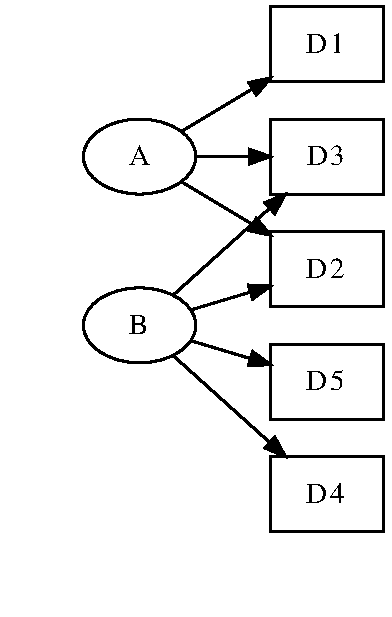
\includegraphics[scale=0.4]{depvis/example-split.pdf}
\hspace{15mm}
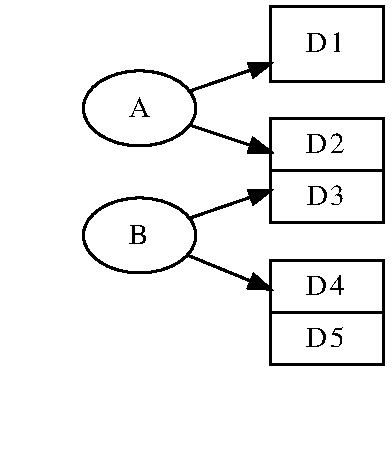
\includegraphics[scale=0.4]{depvis/example-group.pdf}
\caption{Dependency graph without (left) and with (right) grouping of programs
A and B with other DLLs D1 to D5}
\label{fig:grouping}
\end{figure}

In a direct visualization of EXE-EXE and EXE-DLL dependencies,
a directed edge between node $x$ and $y$ denotes that there is
the dependency between file $x$ and file $y$,
e.g. see the left graph in Figure~\ref{fig:grouping}.
This straightforward direct visualization is usually too complex
to be manageable as it often has too many nodes and edges simply
because there are many dependencies in Windows.
For example, in a fresh Windows install,
the {\tt C:/windows/system32} directory alone can contain more
than a thousand DLLs; while in a Windows system with more software installed,
there can be several thousand DLLs.
A simple program such as {\tt notepad.exe} loads more than 30 DLL files.

Thus, a more effective visualization is needed.
We propose a compressed dependency graph with fewer nodes.
This is obtained by grouping the DLL nodes according to the
EXEs which lead to that dependency,
i.e. incoming edges to the binary file.
More specifically, Let the set of all EXEs with a dependency on DLL $x$
be the program set of $x$.
We group all binaries whose program sets are the same.
Figure~\ref{fig:grouping} shows the dependency graph without grouping (left) and
with grouping (right).

Since files often come from particular directories which are either system
directories or program directories and there are different binary types,
we further group files so that the files with the same directory and
same file type are in one node, e.g. label 4 in Figure~\ref{fig:browsers}
which shows the dependencies from DLLs which match with the
pathname {\tt /windows/system32/*.dll} (note that we have used
the forward `{\tt /}' for pathnames).

\paragraph{DLL Dependency Graph}

We define what we mean by EXE-DLL and DLL-DLL dependency in
a {\em DLL Dependency Graph}. The DLL dependency graph
is for a single process, so in the definitions below
we can assume that process $a$ is running executable $x$.

\begin{definition}
An EXE-DLL dependency in a DLL Dependency Graph
is when there is a control transfer from code in executable $x$
to code in DLL $y$.
We say that $x$ has an EXE-DLL dependency on $y$.
\end{definition}

\begin{definition}
A DLL-DLL dependency in a DLL Dependency Graph
is when there is a control transfer from code in
DLL $x$ to code in DLL $y$.
We say that $x$ has a DLL-DLL dependency on $y$.
\end{definition}

A DLL dependency graph shows how the code in DLLs depend
on each other. The motivation is that a DLL often has a certain functionality,
so the graph also illustrates the use of that functionality in an
abstract fashion. Furthermore, DLLs can depend on each other in a complex
fashion which is shown by this graph.
For example, DLL dependency graph can show how a DLL can have
a hidden dependency because it relies on other DLLs for certain functionality.

The DLL dependency graph shows module dependencies during execution
of a program.
In the graph, the nodes are either the single EXE or DLLs.
An edge from node $x$ to node $y$ represents a module or executable
in $x$ calling some code in module $y$.
We also call this as $x$ uses $y$.
Typically this means $x$ calls a function in $y$.
The label of an edge represents the number of invocations, i.e.
the number of calls from $x$ to $y$.
Note that it is possible for DLL $x$ to use DLL $y$ and also for
$y$ to use $x$ during the execution.
In this case, the edge between node $x$ and $y$ is bidirectional.
In the visualization, we use a thick line without any arrow.

A direct visualization of the DLL dependency graph is often too complex,
because there can be too many binaries used during an execution.
For example, Figure~\ref{fig:wget-nogroup} shows the graph for a
small program {\tt wget}.
The graph has too many nodes and edges to be read.
Larger programs generate even more complex graphs, thus we need
a way to reduce the size of the graph.
We use a simple idea that the visualization can be abstracted in two ways
by grouping.
One way of grouping is to group binaries which have a related function
in the same node, for example, we can group Windows DLLs which deal with
networking together.
Another way of grouping is to think of the source of the binary, so this
could be a way of grouping by software vendor.
For example, we can also group binaries which are from Adobe together.

The DLL dependency graph shows actual control flow dependency.
The EXE dependency graph, on the other hand, only shows what
DLLs are loaded. Obviously, in a DLL dependency graph,
if there is a path from executable $x$ to the node representing
DLL $y$ (due to grouping), then there will
be a direct edge in the EXE dependency graph between $x$ and the node
representing $y$ (due of grouping).
However, an edge in the EXE dependency graph does not imply that there is
such a path in the DLL dependency graph, simply because a DLL might
be loaded but not called.
It is useful to be able to tell that a DLL $y$ is not actually called,
although $y$ is loaded.
Such a DLL $y$ is labeled with the notation {\it *y*} in the DLL dependency
graph and is not connected to any other nodes.

To further simplify the visualization, DLLs can have initialization code.
So control flow between EXE and DLLs due to initialization increases
the complexity of the graph. We allow for the visualization to ignore
dependencies which arise due to initialization which can reduce some
of the edges in the graph.
Note that this can lead to some nodes being disconnected from the graph,
and in some cases, those nodes will be treated as nodes which are not called,
i.e. labelled as {\it *y*}.
Our visualization can choose to either ignore DLL initialization or
to take it into account.

\subsubsection{Other DLL Dependency Graphs}

In addition to the basic DLL dependency graph,
we developed two types of DLL dependency graphs obtained through
{\em diff} and {\em projection} operations.

Sometimes we want to compare two executions of the same executable or
module.
For example, we want to identify which additional binaries are used when
we browse a web page with Adobe Flash versus browsing without Flash.
We can then conjecture that those additional binaries are related to the
Flash component.
We also want to know which additional module invocations/dependencies
are incurred by Flash.
To visualize this,
it is useful to define the graph difference between the two graphs,
which we call {\em diff}.
The diff of graph $A$ and $B$, denoted by $A-B$,
is essentially subtracting graph $B$ from $A$.
The result is that only edges that appear in $A$ but not in $B$ appear
in the resulting {\em diff} graph.
A DLL $x$ which only appears in $A$ but not in $B$ is annotated
as {\it +x+}.

Sometimes we want to focus on a specific binary - or a group of binaries.
For example, we want to know which binaries are used by the cryptography
library {\tt crypt32.dll}, and correspondingly,
which binaries use {\tt crypt32.dll}.
We want to determine not only which binaries are directly used,
but also those which are indirectly used.
We propose the {\em projected} DLL dependency graph for this purpose.
In the graph projected on a set of binaries $S$,
only binaries that are used by $S$ or binaries that use $S$ either directly
or indirectly are shown.
Note that this is not the same as finding connected components containing
$S$ in the dependency graph.
This is because the dependency graph loses some information.
Instead, the projection looks at the control flow chain during
execution and selects all the DLLs which have $S$ in its path.
Since projection removes edges from the original graph, we have the
option to keep DLLs which are not in the projection but are used
(this makes sense under grouping) and we label the node as {\it \#y\#}

\begin{figure}
\centering
\begin{minipage}[t]{3.5cm}
\begin{verbatim}
void main (void) {
   A();
   B(1);
}
void C (void) {}
void D (void) {}
\end{verbatim}
\end{minipage}
\hspace{2.0cm}
\begin{minipage}[t]{3.0cm}
\begin{verbatim}
void A (void) {
   B(0);
}
void B (int i) {
   if (i) D();
   else C();
}
\end{verbatim}
\end{minipage}
\caption{Each function is in its own DLL}
\label{fig:indcalls}
\end{figure}

The following example illustrates why the difference between
projection and connected components in the graph.
The program in Figure~\ref{fig:indcalls} has
five functions which are in DLL modules of the same name.
Suppose we project on {\tt A.dll}.
Only {\tt main.exe} uses {\tt A.dll} directly.
{\tt A.dll} uses {\tt B.dll} (directly) and
{\tt C.dll} (indirectly).
{\tt D.dll} is used by {\tt B.dll} but never by {\tt A.dll} at runtime.
Thus, the projection on {\tt A.dll} does not contain {\tt D.dll} even though
it is reachable from {\tt A.dll} in the DLL dependency graph.


\subsection{Explaining the Visualizations}

\begin{figure}[tbh]
\centering
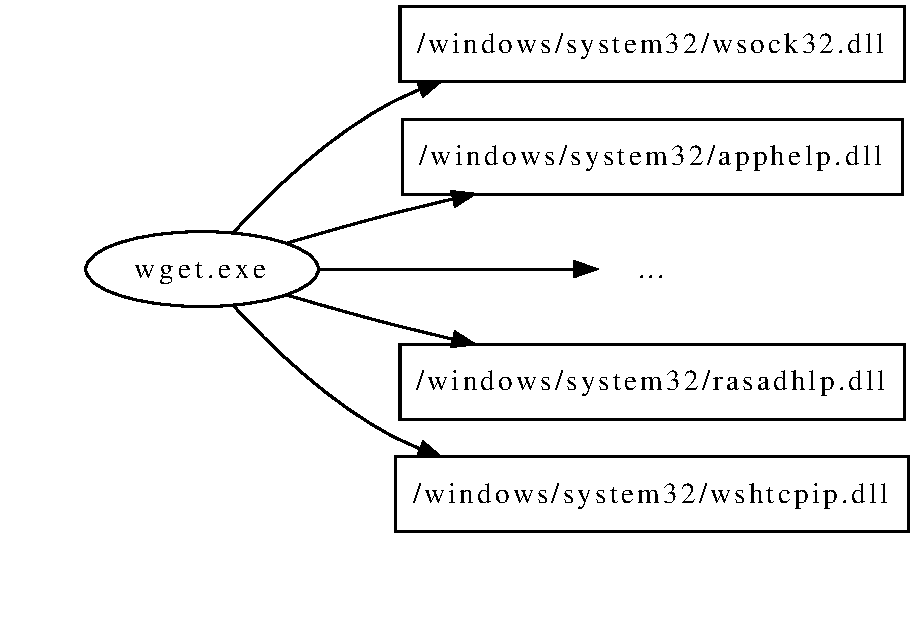
\includegraphics[width=0.6\textwidth]{depvis/wget-exe-split.pdf}
\caption{EXE dependency graph of wget}
\label{fig:wget-exe-split}
\end{figure}

We illustrate the two dependency graphs on a small example, namely, the
{\tt wget} program downloading an {\tt https} page.
Figure~\ref{fig:wget-exe-split} shows the EXE dependency graph for {\tt wget}.
{\tt wget} loads 34 DLLs but due to space limitations,
but the figure only shows 4 of them for simplicity.
The EXE dependency graph is meant for comparing multiple EXE's to show
grouped dependencies.
When there is only a single EXE in the graph, it reduces to a single level
tree. See Fig \ref{fig:boot} and \ref{fig:browsers} to see the graph
when there are multiple EXEs.

\begin{figure*}[htb]
\centering
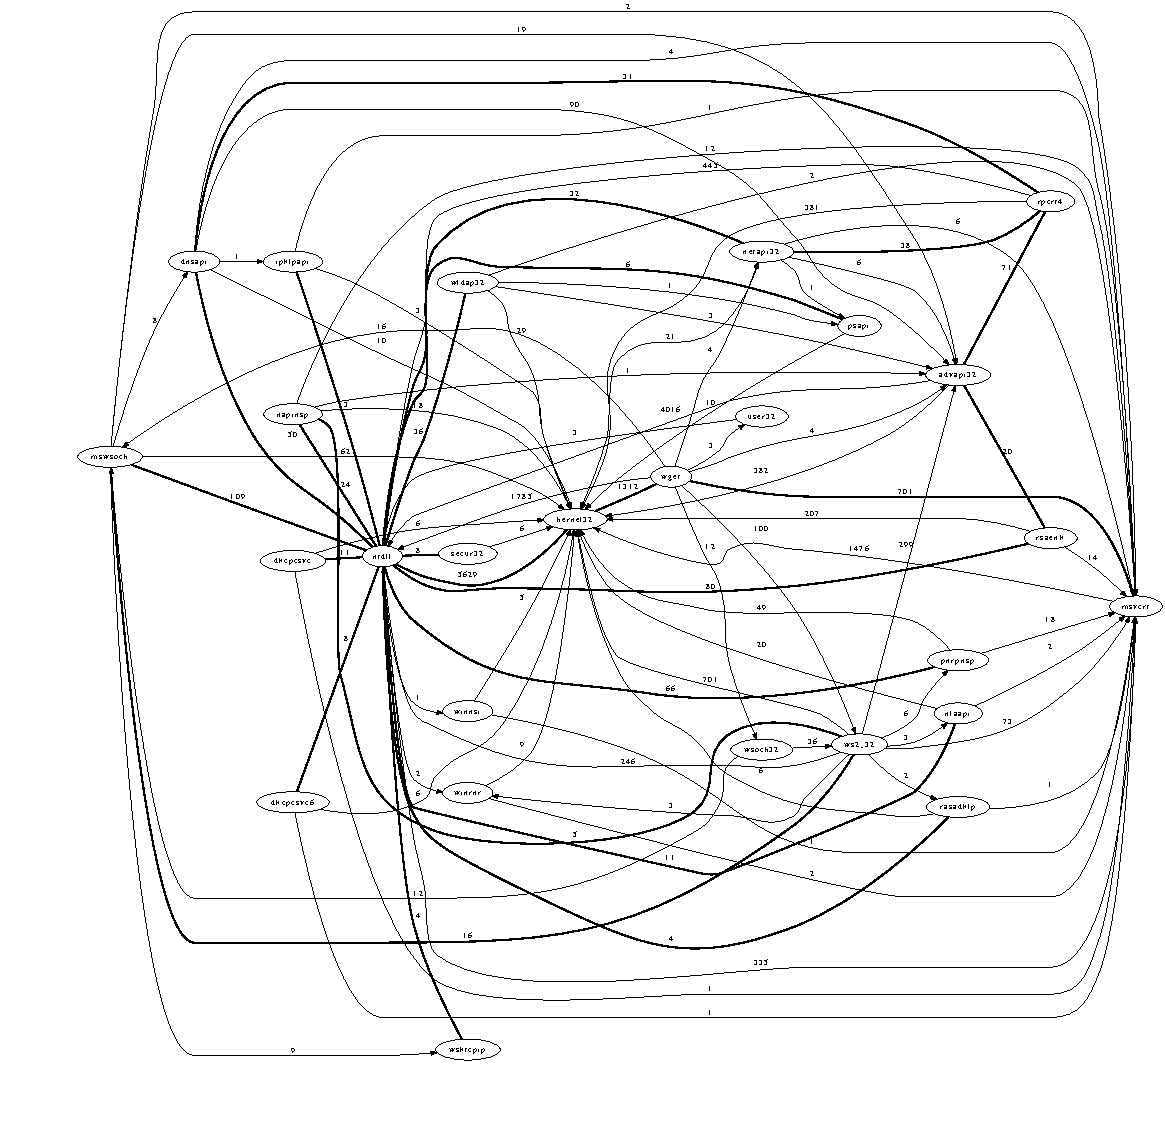
\includegraphics[width=1.0\textwidth]{depvis/wget-nogroup.pdf}
\caption{DLL dependency graph of {\tt wget} without grouping}
\label{fig:wget-nogroup}
\end{figure*}

\begin{figure*}[thb]
\centering
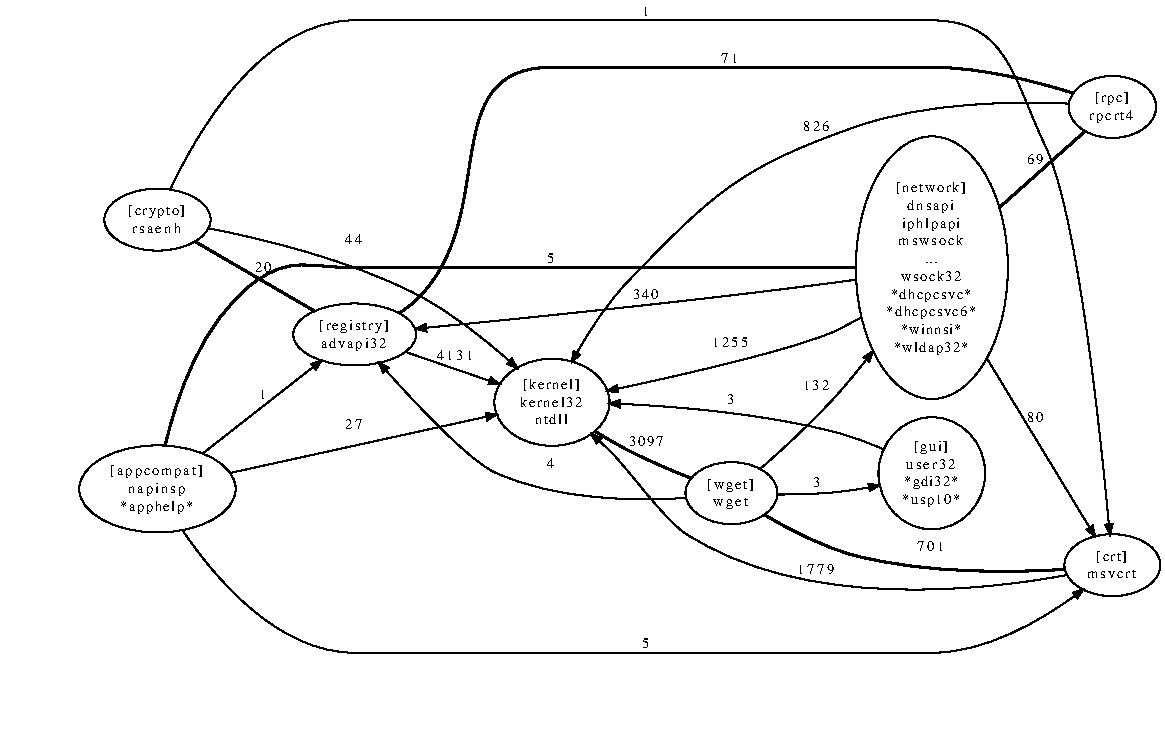
\includegraphics[width=1.0\columnwidth]{depvis/wget-function.pdf}
\caption{DLL dependency graph of {\tt wget} grouped by functionality}
\label{fig:wget-function}
\end{figure*}

Figure~\ref{fig:wget-nogroup} shows the DLL
dependency graph for wget without grouping; while
Figure~\ref{fig:wget-function} shows it grouped by functionality.
As we can see, Figure~\ref{fig:wget-function} is much more compact
because the nodes have been grouped according to the function of the modules.

We manage the assignment of files to groups with a data\-base which is
used by the visualization program.
A table in the database has three fields: binary,
grouping method and group name.
Each binary file is assigned to a group under each grouping method.
For example, the binary {\tt user32.dll} is assigned to group {\tt gui} under
the grouping method {\tt functi\-onality}.
As there is no single source of information for all the binaries, we mainly
searched on the Internet for information using the binary's name.
We also used the DLL's exported functions and file version metadata
as heuristics.

For vendor grouping, the assignment of most binaries was done automatically
using the ``Company'' information embedded in the file version metadata.
In some cases, some binaries do not have metadata, so a manual process
was used.
One can also have other and multiple mappings beyond the two which we used.
In this work, we only used a
common mapping for functionality and vendor mappings
in all the dependency graphs.
The grouping process as a whole is relatively static and can mostly be
done once so while some manual effort is needed to create an initial
database, the database may only need to be updated infrequently.

Figure~\ref{fig:wget-nogroup} shows the interactions
between the various DLLs used by {\tt wget}.
It illustrates that a small program already
gives a complex dependency graph.
As such, it may be more useful to check some specific details.
Figure~\ref{fig:wget-function} gives
a ``big picture'' of the dependencies
in {\tt wget} in terms of how the various functional
components interact.
We see that a number of DLLs are loaded but not used in our https download
(files of the form {\it *x*}).


\subsection{Implementation}

Implementation of the visualizations entails collecting tra\-ces when
binaries are loaded and tracking of function call and return.
Binary loading information is obtained using
a modified version of WinResMon~\cite{ramnath2006winresmon},
which makes use of a kernel driver to obtain
what binaries are loaded by a process as it runs and
what child processes are created.
The EXE dependency graph is created from
the WinResMon trace file into a dependency graph in
Graphviz \cite{ellson2002graphviz} format and rendered by {\tt dot} in Graphviz.

The system trace from WinResMon is very robust and allows for continuous
full system tracing if so desired.
It can also trace a large portion of the system boot,
see Fig. \ref{sec:apply:boot}.
It also works with software which employs self-modifying
code and other malware techniques to defend against virtual machines,
debuggers and code instrumentation such as Skype.
Thus, it can handle many more cases than with a more detailed
instruction instrumentation or interpretation approach, as is done
with PIN below.

The DLL dependency graph is built from a runtime control flow trace from
function calls and returns during execution.
We employ PIN~\cite{luk2005pin} which instruments the binary to allow monitoring
of the control flow during execution of call and return instructions
when a process runs saving these events into a trace file.
The trace is then analyzed to generate a DLL dependency graph in
GraphViz format.

The DLL dependency graph only needs instrumentation of the call instructions
which is straightforward.
DLL projection, however, requires tracking of the control flow of both
call and return instructions.
The full call/return tracking is more complex than one would expect
under Windows because one has to handle:
non-local goto's from {\tt setjmp()} and {\tt longjmp()}, exception handling,
kernel callbacks and multithreading.
For example, a naive implementation which matches counts of call and
return instructions will fail when a {\tt longjmp()} is used
since that means that some function does not return.
We make use of stack and return address matching to do this
tracking, which is not described in detail for lack of space.

In Windows, execution can be interrupted to switch to a new context.
When execution in the new context completes, execution of the original
context resumes.
There are a number of reasons why the context changes
such as: asynchronous procedure call (APC), kernel callbacks
(kernel calls a user function) and structured exception handling.
Thus, context switching has to be tracked to avoid matching
call and return from different contexts.
We remark that the start of a context switch can be obtained in PIN but
not when the context terminates.
Instead, termination is observed by watching the {\tt NtCallbackReturn}
and {\tt NtContinue} system calls.
Context switching can be cascaded, thus, we maintain the unfinished
contexts in a stack.

We generate a trace file to record the call/return control flow.
The trace records events such as function calls/returns,
thread creation/termination, context switching, binary loading
and system calls.
This allows us to analyze the execution trace in many ways to generate
different graphs.

The DLL initialization in Windows is identified by the special
DLL entry function {\tt DllMain} which is called when a DLL is loaded.
To remove the control flow effect due to DLL initialization,
we remove all calls which are due to execution of {\tt DllMain}.

\subsection{Comprehending Module Dependencies in Real Software}
\label{sec:apply}

We now give some usage scenarios which demonstrate how our visualizations
make it easier to understand the web of dependencies of software in Windows.
The dependencies shown are from programs runs in each
example and show how programs and binaries used in those runs
relate to one another.
The figures in this chapter are all scalable and thus can be magnified
in the PDF to see more detail and we encourage readers to do so.
In this section,
the files in some nodes in the graphs are abbreviated to $(\ldots)$ to make
it easier to fit the graphs in the thesis.
All the DLL dependency graphs remove dependencies due to
DLL initialization.\footnote{
One could choose also to see DLL initialization dependencies, as removal
would not make sense for DLLs which do significant work in the initialization.
}

\subsubsection{System Boot}
\label{sec:apply:boot}

\begin{figure*}[htbp]
\centering
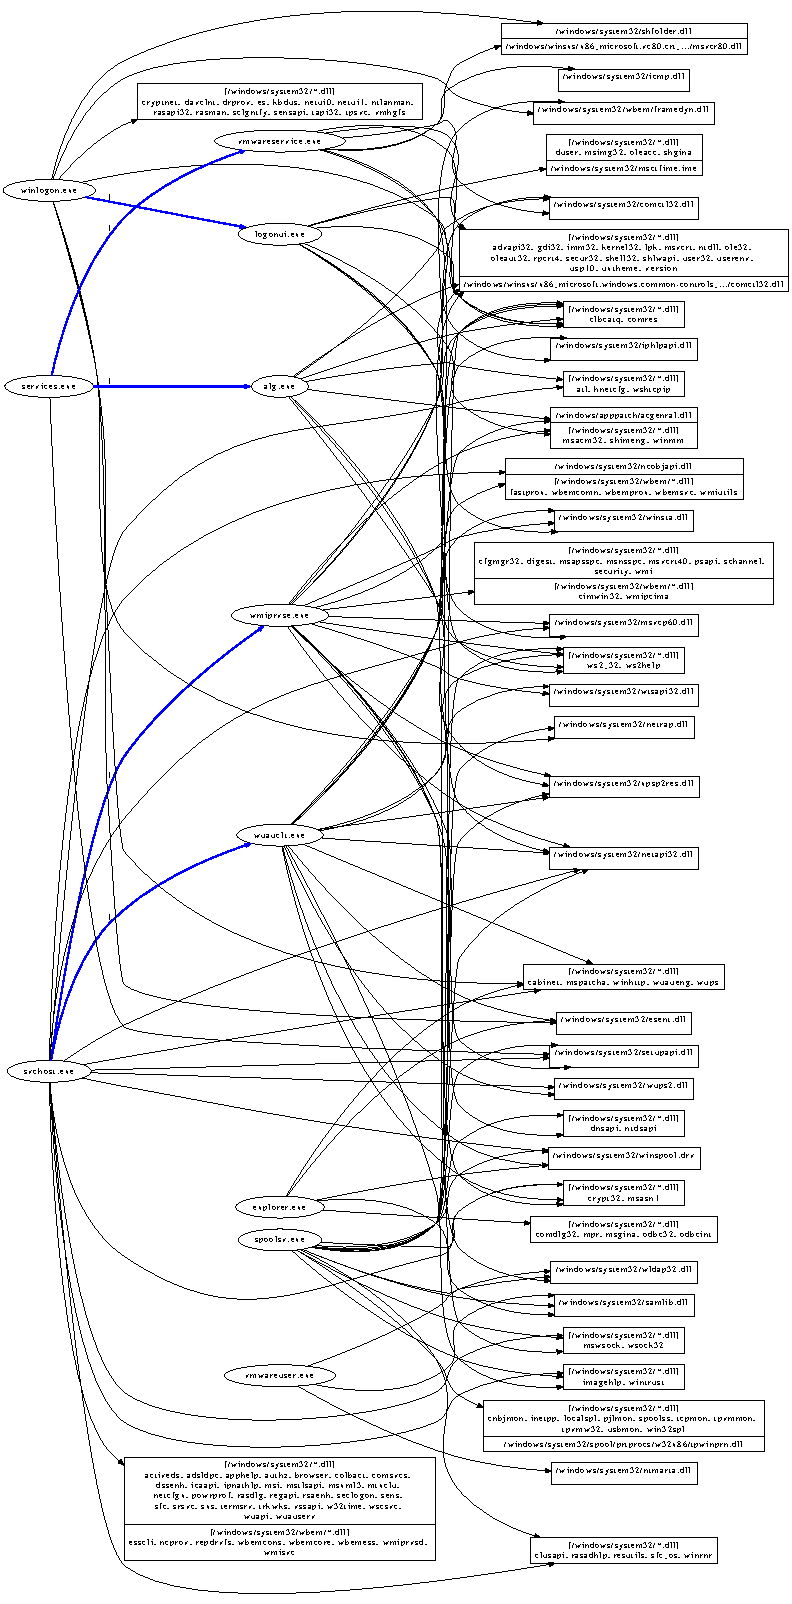
\includegraphics[keepaspectratio,width=0.95\textwidth,height=0.95\textheight]{depvis/boot-gdll.pdf}
\caption{EXE dependency graph of the whole system}
\label{fig:boot}
\end{figure*}

Figure~\ref{fig:boot} shows the EXE dependency graph for a boot to shutdown cycle
for a fresh Windows XP install.
The machine was booted and automatically logged in,
then logged off, and shutdown. One might expect that the processes
form a process tree but that is not the case because some of the processes (e.g
svchost, winlogon, services) start before our monitoring tool
(WinResMon) does. Looking at the big picture of the startup and shutdown
process, it can be seen that some DLLs are shared by many programs (e.g
{\tt kernel32}, {\tt gdi32} and this is expected since system calls would use
{\tt kernel32} while GUI programs would use {\tt gdi32}).
On the other hand, some DLLs are used exclusively by one program (e.g.
{\tt odbc32} is used only by {\tt explorer}).
This is somewhat surprising leading to the question why {\tt odbc32},
the database query interface, is used by {\tt explorer}.

\subsubsection{Comparing Web Browsers}

\begin{figure}[bthp]
\centering
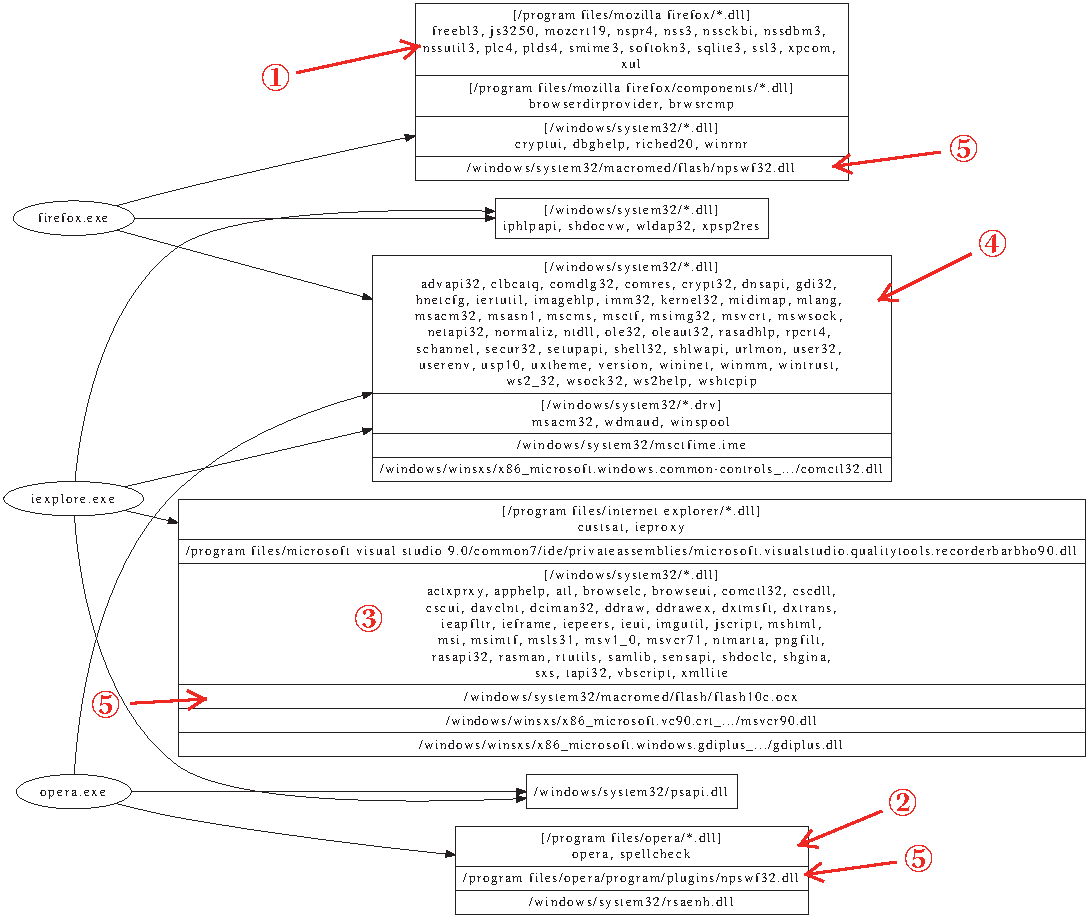
\includegraphics[width=1.0\textwidth]{depvis/browsers-group-annot.pdf}
\caption{EXE dependency graph of three browsers: IE, Firefox, Opera}
\label{fig:browsers}
\end{figure}

\begin{sidewaysfigure}
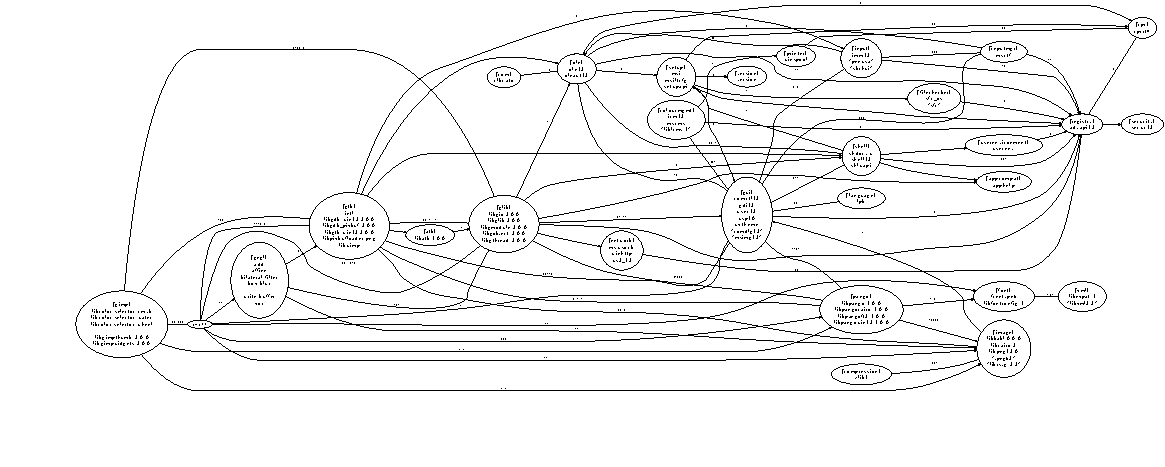
\includegraphics[width=1.0\textwidth]{depvis/gimp-function-removed.pdf}
\caption{DLL dependency graph of Gimp grouped by functionality}
\label{fig:gimp-function}
\end{sidewaysfigure}

Figure~\ref{fig:browsers} shows the EXE dependency graph for three
brow\-sers: Internet Explorer, Firefox and Opera.
Each browser displayed a YouTube page to play a
video till completion. The scenario is intended to show the dependencies
of the binaries used by the three programs
with similar function but different source code base.
The visualization shows the commonalities and differences
between the software modules in the three browsers.
It also shows dependencies on other software which is not part of
the browser code base and
which comes in through the use of browser extensions or plugins,
e.g. Adobe Flash.

This example shows the compressed EXE dependency gra\-ph
with grouping.
We see that grouping makes the graph easier to visualize.
Firstly, the grouped version is much smaller in size.
Secondly, it is easier to identify which binaries are shared by the same programs.
We have highlighted particular nodes in the graph with
labels, the numbered red arrows, discussed below:
\begin{itemize}


\item Labels 1, 2 and 3 show the DLLs used exclusively by Firefox, Opera
and Internet Explorer respectively. Opera does not have many  of its own DLLs.
On the other hand, Firefox uses its own DLLs (in {\tt /program files/mozilla firefox}) for many features.
In the case of Internet Explorer, the ownership of the DLLs are less clear
since most of the DLLs used come from the {\tt system32} directory.
This may be due to the deeper integration of Internet Explorer with
Windows.

\item Label 4 shows the common binaries shared by all three browsers.
It is not surprising that a large number of binaries are shared.
This is because most of the major Win32 API calls
are implemented in those binaries, e.g.
\texttt{msacm32.drv} and \texttt{wdmaud.drv},
are the audio drivers that all browsers use to play the video.


\item Label 5 shows the different ways that each browser runs Flash.
In Internet Explorer,
Flash is installed as an ActiveX control (\texttt{flash10c.ocx}).
Firefox and Opera both use (\texttt{npswf32.dll}), the Flash plugin
for Netscape. We discover that the same DLL is duplicated in
different directories.

\end{itemize}

\subsubsection{Gimp}

\begin{sidewaysfigure}
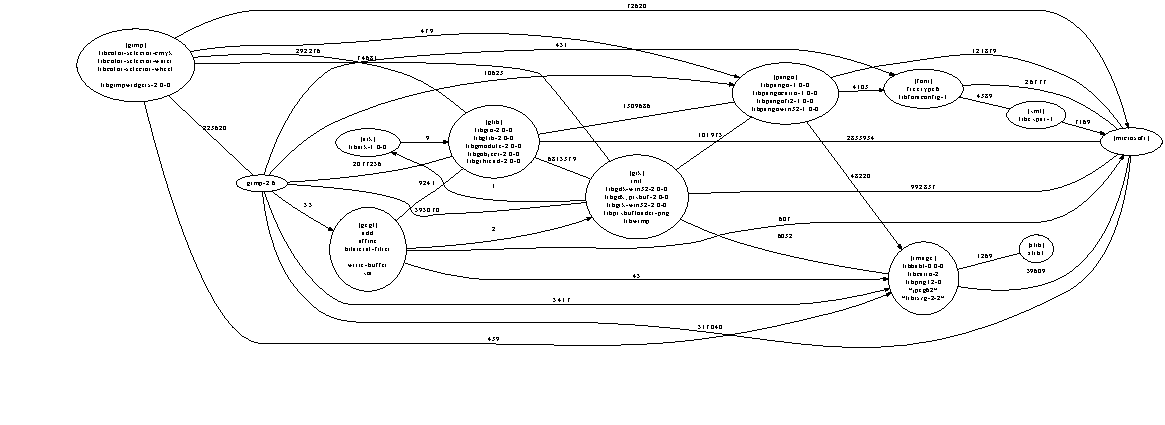
\includegraphics[width=1.0\textwidth]{depvis/gimp-vendor.pdf}
\caption{DLL dependency graph of Gimp grouped by software vendor}
\label{fig:gimp-vendor}
\end{sidewaysfigure}

GIMP is an open source image manipulation program. Like many open source
software, it uses libraries from various sources. In this experiment, we
executed GIMP without opening any files. We want to see how GIMP uses various
libraries and the interactions between them.

Figure~\ref{fig:gimp-function} shows GIMP grouped by functionality while
Figure~\ref{fig:gimp-vendor} shows
GIMP grouped by software vendor.
GIMP is large but quite modular. The bulk of
the DLLs used are from the GEGL, GTK and GLIB frameworks. It also uses the
Windows GUI APIs (e.g., gdi32, comctl32) extensively.

Figure~\ref{fig:gimp-function} is a larger graph than Figure~\ref{fig:gimp-vendor}
but is still understandable using the functional grouping,
e.g. {\tt gimp} uses the {\tt [gegl]}
image processing modules, which in turn uses the {\tt [gtk]} windowing
module.  The remaining DLLs are not used very much.

Figure~\ref{fig:gimp-vendor} is interesting because it shows that
many different software vendors/providers are used in GIMP.
Microsoft is also prominent but is
expected since GIMP is running on Windows and uses the Win32 API.
The presence of so many different software vendors could also make
troubleshooting difficult since it might be difficult to determine
which vendor is responsible if GIMP behaves in unexpected ways.
Figure~\ref{fig:gimp-vendor} also shows
one of the advantages of open source software, namely, reuse. The
binaries belonging to GIMP only turn out to be quite small and
GIMP prefers to rely on
existing frameworks like {\tt gtk} (GUI) and GEGL (image processing).

\subsubsection{Firefox: Plug-ins and a Surprise}

\begin{figure}
\centering
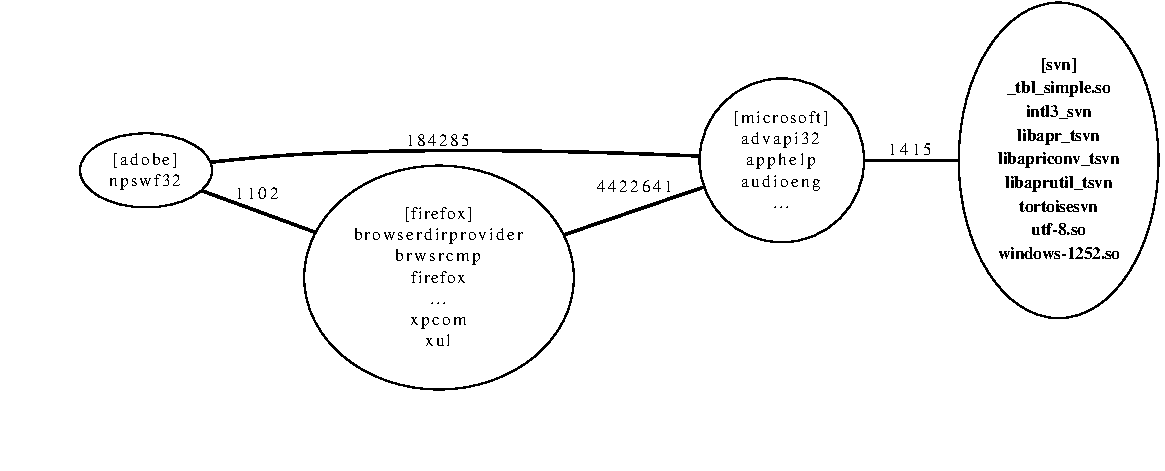
\includegraphics[width=1.0\columnwidth]{depvis/firefox-vendor.pdf}
\caption{DLL dependency graph of Firefox grouped by software vendor}
\label{fig:firefox}
\end{figure}

Firefox allows extensions through its own plug-in architecture.
Figure~\ref{fig:firefox} shows the DLL dependency graph
of Firefox as grouped by vendor. We find a node for Adobe.
This is because {\tt npswf32} is the Flash plugin for firefox.

We discover a surprising node -
the {\tt svn} vendor group (shown in bold font) which is to do with
the TortoiseSvn interface to SubVersion (the version control system).
TortoiseSvn is unrelated to either Firefox plugins or addons.
Thus, one might find its presence strange, when Firefox is being executed.
The explanation lies in the way the Tortoise shell extension
behaves in Windows. TortoiseSvn injects its DLLs into the
{\tt Explorer} shell process when Windows starts.
When explorer runs a process, the TortoiseSvn
DLLs are also loaded into the new process.
The fact that there is interaction with a module which is not part of
the Firefox can mean that a bug in that module can also affect Firefox.
This can be concern for software developers.

\subsubsection{Adobe Flash in Internet Explorer}
\label{sec:flash}

\begin{figure}
\centering
\noindent\makebox[\textwidth]{
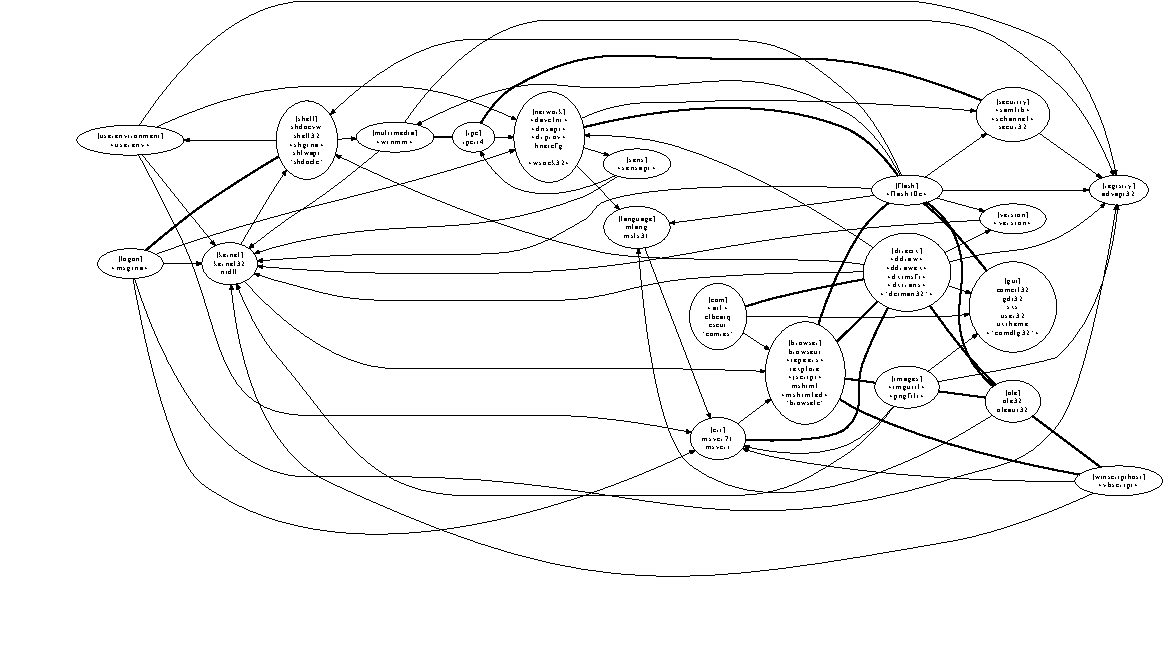
\includegraphics[width=1.2\textwidth]{depvis/ie-yt-diff.pdf}
}
\caption{Diff of DLL dependency graph of Internet Explorer with Flash and without}
\label{fig:ie-diff}
\end{figure}

This scenario is to understand the interaction of Adobe Flash in
the Internet Explorer browser.
The strategy used here is to compare two DLL dependency graphs,
Internet Explorer opening a website with flash content and
Internet Explorer showing the {\tt about:blank} page since
{\tt about:blank} page is the most minimal webpage for Internet Explorer,
Figure~\ref{fig:ie-diff} shows the difference (diff) between these two
graphs.
The DLLs marked with {\bf +x+} are the {\em extra} DLLs loaded
when Flash is played.
Most of these extra DLLs fall into the
network, multimedia, DirectX and Flash categories.

\begin{sidewaysfigure}
\centering
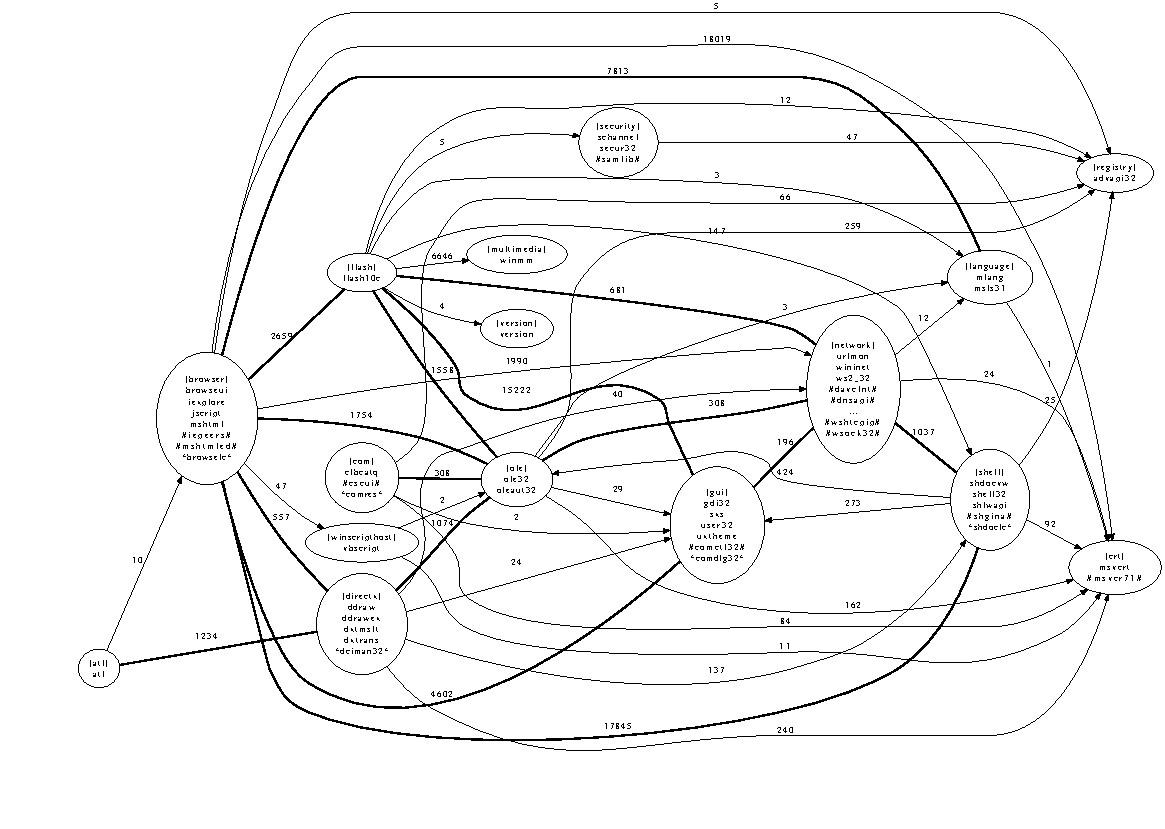
\includegraphics[keepaspectratio,width=0.8\textwidth,height=0.8\textheight]{depvis/ie-yt-proj.pdf}
\caption{Projection of the DLL dependency graph of Internet Explorer on Flash}
\label{fig:ie-proj}
\end{sidewaysfigure}

To further investigate the interactions resulting from the Flash module,
we project the visualization on {\tt flash10c.ocx} which is
the Flash ActiveX control.
Figure~\ref{fig:ie-proj} shows the projected graph.
We can see that Flash is interacting with the browser and multimedia modules.
The DLLs marked with {\bf \#x\#} neither use {\tt flash10c.ocx}
nor are they used by {\tt flash10c.ocx}.
In the {\tt network} group,
we can see that {\tt wsock32} is marked by {\bf \#x\#} but
{\tt ws2\_32} is not.
Windows has many network modules as shown in the {\tt network} group.
{\tt Wsock32} is an
older version of the winsock modules whereas {\tt ws2\_32} is the newer version.
This means the Flash player only uses the latest version of winsock rather
than the older version which is closer to the Unix socket API.
However, the older version is still used by some other modules
because otherwise {\tt wsock32} would have been labelled as {\bf *x*}.
The EXE dependency graph of the three browsers also shows that
both winsock modules are loaded by all three browsers.
The difference with projection is that projection is
more precise and shows the interaction between
the Flash module with the particular network module.

\subsection{Conclusion}

\TODO{Commented out the following. Can optionally add to previous section.
In addition to the scenarios in Sec.~\ref{sec:apply},
we experimented with other scenarios which we describe briefly due to lack
of space. They are similar to those in Sec.~\ref{sec:apply} but the details differ.
We investigated what happens with Internet Explorer under
the following situations:
(i) loading a Java applet versus an {\tt about:blank} page;
(ii) a demonstration Microsoft Silverlight webpage versus blank; and
(iii) a {\tt https} webpage versus regular {\tt http}.
Another scenario is to answer the question of
what are the new dependencies for Acrobat on a regular PDF versus
one with an embedded form.
We also experimented with Java applications and .NET applications
to see the behavior of virtual machines and managed code.
}

The two visualizations EXE dependency and DLL dependency graphs are just two
ways to visualize software module dependency using execution traces.
We can have other different visualizations using the traces.
For example, instead of using binaries as basic units, we can use functions
to visualize more fine grain behaviour.
This makes the graph much more complex because there are many more functions
than binaries.
We can use similarity grouping, diff and projection to ``zoom in''
on specific regions.
Because we utilize instrumentation of binaries, we can also visualize other runtime
properties of the code.
For example, visualize the CPU time used by different modules,
and scale the nodes in the graph so that the area of each node is proportional to the time
(or instructions) spent in the binaries represented by the node.

Although we have focused on visualizations, the traces which are collected
contain a wealth of information. A workflow for software comprehension can also make use
of the trace data in addition to the visualization.
The trace data is at a fine grain level but is hard to understand.
Thus, the visualization gives a roadmap for investigating the traces.

We have demonstrated that software dependencies in Windows are quite
complex even when looking at the coarse grain level of software components
packaged into binaries and executables.
Our tools give an effective way of extracting and
visualizing the software dependencies and interactions between binaries.
We show that even with the complexity of actual Windows software,
it is possible to analyse whole system interaction,
understand how modules are used and shared,
and also discover potential unexpected or unusual interactions/modules.
Such an understanding is also useful for software developers,
system administrators and also users, to manage the
software ecosystem on Windows and to deal with the problems which arise
from module updates and potential ``DLL hell'' repercussions.


\clearpage
\clearpage
\section{Visualizing Windows System Traces}
\label{sec:lviz}

% \subsection{Introduction}

Software is increasingly complex with many interactions with other software
and the operating system.
The previous visualization shows the complexity in the
aspect of module dependency.
Other factors include persistent state interaction, inter-process communication,
networking, etc.
This complicates understanding software/component behavior and diagnosing
problems or performance.
As discussed in Section~\ref{sec:bg-win},
the close source nature of Microsoft Windows (or simply, Windows)
exemplifies this trend.
Suppose our task is to understand/diagnose/debug some software on Windows.
Ideally, system/software documentation or source code
analysis would give the answer.
In practice, however, this may not be
workable either due to lack of source or overall
system complexity being too high.
An orthogonal approach to address this issue is by examining
detailed system behavior.
Recently, there are a number of monitoring systems which
give detailed system traces such as DTrace~\cite{cantrill2004dynamic} for Solaris,
DProbes for Linux and Flight Data Recorder~\cite{verbowski6flight}
and WinResMon (Sec.\ref{sec:winresmon}) for Windows.
However, as shown earlier in this chapter,
the system traces can be very large and also
difficult to analyze.

We propose \code{lviz}, a visualization tool for
understanding such large and complex system traces.
\code{lviz} has a number of visualizations.
In the thesis, we focus on the visualization which we call VDP.
It consists of a number of inter-connected sub-visualizations:
an extended DotPlot;
two Axis Histograms; and one or more barcodes.
The VDP can be flexibly configured for different purpose.
In Section~\ref{sec:lviz-vis}, we show the design and configurations of VDP.
In Section~\ref{sec:lviz-imp}, we show that
the prototype of \code{lviz} is efficient and can handle large system traces
with real-time response. For example, a trace of size 120MB with 558K events 
is loaded in under 3 seconds
and after that it can be interactively displayed/zoomed in around 0.5 seconds.
The VDP can be used on different traces and for different purpose
by using different configurations.
In Section~\ref{sec:lviz-study}, we use some case studies to show that
VDP can be used for solving performance problems,
program failure diagnosis and finding execution patterns/anomalies.

\subsection{Related Work}
\label{sec:lviz-related}

% \TODO{maybe dont need the first para}
% There are a number of related works on execution trace visualization,
% some are graph based, some are hierarchical,
% some are Cartesian coordinate based.
% We focus on Cartesian coordinate base visualization to which VDP belongs.
% The Cartesian coordinate based visualization is commonly used when each
% visualized entity (function, event, object, line of source code, etc.)
% is associated with some numerical properties.
% Each entity is then positioned on to the Cartesian coordinate based on
% its properties.

% \TODO{reviewer 2:
% The statement in section 2 that Cartesian visualizations are commonly used
% when each visualized entity is associated with two or three numerical
% properties is somewhat confusing. The choice of the so-called embedding, or
% projection, is in Infovis in general not one-to-one to the data attributes,
% at least not at this level. For example one would visualize some data using
% hierarchies primarily and not Cartesian plots if the most important aspect to
% reason about is the hierarchical one, even when the data has 2 or 3 numerical
% attributes per element. Or a table in a data base can be shown as a table,
% but better as a graph, if it actually encodes a graph. I think strongly that
% the layout choice should reflect the task at hand, and not data modeling
% issues.  fixed.
% }

% \TODO{reviewer 2:
% In the previous work you should definitely discuss the more recent work of
% Holten, Cornelissen, van Deursen, and Zaidman on visualizing trace
% information, see "Understanding Execution Traces Using Massive Sequence and
% Circular Bundle Views" (proc. ICPC 2007), since it is at least as related to
% the topic of this paper as the other references, and is quite recent. The
% work of F. van Ham and J. Abello on MatrixZoom fits also in this area.  fixed
% (only added the first paper).
% }

SeeSoft~\cite{eick1994graphical} visualizes general log files by zooming out
lines of text logs and coloring them by message types.
SeeLog~\cite{eick1996displaying} visualizes Unix accounting trace files by
plotting events by time and process.
SeeLog can be viewed as a restricted variant of the
VDP visualization.
Magpie~\cite{barham2004using} is a performance analysis tool designed for web
servers.
It uses collected system events including file I/O, computation,
thread scheduling and network to analyze the resources usage of
HTTP requests.
BootVis~\cite{bootvis} 
is a visualization tool to tune
Windows booting plotting resource use versus time.

Bodic et al.~\cite{bodik2005combining} propose another visualization tool for
web servers.
It shows frequency of different HTTP requests
and highlight anomalies that may indicate site failures.
VDP on the other hand is a general trace visualizer but
it can be used for similar diagnosis (see Sec.~\ref{sec:wbbench}).
TuningFork~\cite{bacon2007tuningfork} is a trace analysis tool for real-time
systems including visualizing unsatisfied real time constraints in real-time
systems.

EVolve~\cite{wang2003evolve} is a visualization framework for understanding
Java program by visualization execution traces from the JVM and
has a DotPlot visualization.
% It includes a DotPlot module which has some similarity with VDP.
However, VDP uses an extended DotPlot (see Sec.~\ref{sec:lviz-vis})
and generates different visualizations (see Fig.~\ref{fig:make-matching})
depending on its configuration.
\code{lviz} is designed to scale for large traces and
to be efficient to meet user interaction needs.
Voigt et al.~\cite{voigt2009object} propose a visualization method which correlates
class method invocation, object invocation and time.
To correlate methods and objects, it places objects and methods
on each axis and draw dots to represent the
method-access-object relationship.
Cornelissen et al.~\cite{cornelissen2007understanding} propose two visualizations,
massive sequence and circular bundle views, to examine execution traces.
The massive sequence view visualizes a trace by placing each event as rectangles
according to its invoking software module (X-axis) and time (Y-axis).
The circular bundle view visualizes software module interactions by arranging
modules into a tree and draw two-module interaction as a curve along the
path in the tree.
These visualizations are different as they do not compare events 
nor work with closed source software.

% \TODO{reviewer 3:
% Dotplots and their extensions have been studied in the field of visualization
% more than extensively. They have been proven to be useful for finding
% patterns in similarities in various fields. In this paper, the dotplot is not
% used differently. The configuration of visualizations reminds me DNAVis: Case
% Study: Visualization of annotated DNA sequences, Tim Peeters, Mark Fiers,
% Huub van de Wetering, Jan-Peter Nap, Jarke J. van Wijk, Joint Eurographics
% IEEE TCVG Symposium on Visualization (2004).
% }

\subsection{System and Visualization Design}

% \TODO{reviewer 3:
% Look at the order of the figures, they do not appear in the same order as they appear in the
% text. Also, they are not as close as possible to the reference in the text.
% }

We describe the design of \code{lviz}, a system for visualizing Windows system
traces.
% \footnote{
% \code{lviz} has a number of visualizations. In this work, we focus on the VDP
% visualization.
% }
We emphasize that the visualization proposed
is not specific to Windows as traces from other operating systems
can be used as well.
\code{lviz} can be easily adapted to read traces in other format,
which make it friendly to other monitoring systems such as DTrace
and SystemTap.

\subsubsection{System Traces}
\label{sec:systrace}

Our objective is to visualize detailed system traces.
In the rest of the section, we will shorten system trace to simply trace.
Our traces are obtained with WinResMon (Section~\ref{sec:winresmon}) which
captures all operations performed by the Windows kernel
from all processes.
% Our aim is to capture the relevant operations which can be attributed
% to interactions between software (system and applications).
% Collecting trace events in Windows is much harder than UNIX.
% Windows NT (Server 2000, XP, Server 2003, Vista) is a microkernel
% based operating systems.
% Programs are usually written for the Win32 API but those are decomposed
% into microkernel operations.
% However, as Windows is closed source,
% only the Win32 API is documented and not the microkernel API.
% We use WinResMon~\cite{ramnath2006winresmon} to capture system trace.

A WinResMon trace consists of four classes of events
due to operations on processes, files, network and the registry.
An event contains the following properties: (the example events
in Figure~\ref{fig:logex} use the ordering below)
\begin{tightitemize}
\item {\bf PID/TID} is the ID of the process/thread which
performs the operation.
%Since it is reusable, it is not unique over time.
\item {\bf Program name} is the pathname of the program binary.
%\item {\bf Group name and User name} is the owner of the process.
\item {\bf Group} and {\bf User name} of the process.
%Unlike UNIX, in Windows there are multiple privileged users.
% where root is the only privileged user,
% in Windows there are more than one privileged user, such as
% ``{\tt NT AUTHORITY\BS SYSTEM}'',
% ``{\tt NT AUTHORITY\BS LOCAL SERVICE}'',
% ``{\tt NT AUTHORITY\BS NETWORK SERVICE}''
% and arbitrary number of administrators.
\item {\bf Start and end times} of the event.
% are 64-bit timestamps derived from the Intel processor performance counters.
% % are 64-bit timestamps generated by the RDTSC~\cite{rdtsc} instruction.
% % \TODO{This timestamp is a relative timestamp counting from CPU reset.
% % CPU reset may be triggered by system boot or waking up from hibernate,
% % thus one has to add addition bits to ensure monotone increasing timestamp.}
% \TODO{usenix comm:
% A minor technical tidbit: in Section 3.1 it is said that start and end time of
% the event is recorded using CPU perf counters; what happens in SMPs? How is
% the timestamp decided?}
\item {\bf Operation type} is specific to the event.
Some examples are given below.
\item {\bf Operation parameters}: The semantics depends on the operation type,
e.g.  resource pathname, file access flags, etc.
% and I/O data.
%Collecting I/O data can be turned on/off by command line options,
%as it is comparably expensive.
%The maximum size of I/O data can also be adjusted.
\item {\bf Return value} from the operation
is either success or an error number explaining why the operation failed.
\item {\bf Call stack trace} of the process which generated the event.
In this work, we use the deepest function call
from the corresponding executable, i.e.
excluding functions in libraries,
but one could also use the full stack trace.
This information is useful to associate a program point in the
application code with the event.
\end{tightitemize}

% There are 46 operation types in total, 6 related to file,
% 7 related to registry, 5 related to process, and 28 related to network.
Examples of events are file operations,
e.g.  file\_create, file\_close and file\_read;
registry operations, e.g. reg\_setvalue;
process operations, e.g.  thread\_create;
and network operations, e.g. socket\_bind.
Pathnames of files and registry keys are recorded as operation parameters.
Additional information depending on the specific operation is also recorded.
For example, file\_create, which represents both opening an existing file
and creating a new file, the operation parameters include the pathname of
the opened or created file, access flags, file attributes, creation disposition
(create new, open existing,
% truncate existing, or append to existing files),
etc.) and other Windows operating system specific information.
Figure~\ref{fig:logex} shows two examples of events.
WinResMon can optionally capture the data associated with an
event. (see Section~\ref{sec:wbbench} which uses network packet data)
% While file and registry resources are represented as paths,
% network resources are represented as network address, i.e. IP address and port.
% Only TCP and UDP protocols are recorded.
% A socket is not associated with an address until {\tt bind()} or {\tt connect()} is called,
% Thus not all network operations are associated with resources.

\begin{figure}
\fbox{\parbox{0.95\columnwidth}{
\tt\small
1268 1732
"C:\BS WINDOWS\BS System32\BS svchost.exe" "NT AUTHORITY\BS SYSTEM"
1098307213586 1098307319878
file\_create
"\BS Device\BS HarddiskVolume1\BS WINDOWS\BS Prefetch\BS NET1.EXE-029B9DB4.pf"
access=0x120089, share=0x0, attr=0x0, cd=0x1, co=0x60, si=0x1
STATUS\_SUCCESS
\vspace*{1mm}

\hrule
\vspace*{1mm}

204 960
"C:\BS WINDOWS\BS system32\BS cmd.exe" "GROUP\BS USER"
1101551207684 1101551216008
reg\_queryvalue
"\BS Registry\BS Machine\BS Software\BS Policies\BS Microsoft\BS Windows\BS Safer\BS CodeIdentifiers"
handle=0x78, name="LogFileName", t=0x0, l=0
STATUS\_OBJECT\_NAME\_NOT\_FOUND
}}
%\caption{Two examples of events (without call stack trace)}
\caption{Two examples of events}
\label{fig:logex}
\end{figure}

% A system trace is stored in a compressed text file, where each line
% records an event.
% We choose this format because it makes filtering and processing easy through
% existing UNIX stream text processing programs.
% The drawback of text file is the difficulty in random accessing,
% however, our visualization programs are implemented to sequentially
% access the trace.

% \TODO{reviewer 3:
% The list in section 3.1 can be compressed and figure 1 can be given inline.
% }

\subsubsection{Trace Visualization}
\label{sec:lviz-vis}

Visualizations for traces need to be able to compress a lot of detail
and yet be usable for illustrating many different
kinds of system behavior ranging from understanding
system administration to debugging to performance evaluation.
% investigating security issues, comparing behavior of program versions, etc.
In order to meet such a wide range of needs, we will see that the visualization
should be adaptable and configurable to show specific aspects for a
given purpose.  It must also be able to scale at different detail levels.

% We describe the design and rationale
% of two novel visualizations: RTG and Extended DotPlot.
% They have different purposes and complement each other.
% Both visualizations are meant for interactive use for exploring different
% ways of looking at the same trace under different visualization
% configurations and zoom levels.
% % modes which also includes
% % interactive zooms to see finer detail.

Our visualizations use color for greater visual
bandwidth as well as customization flexibility.
We support both RGB and CMY color modes.
The RGB color mode displays events on a black background
and is appropriate if the visualization is displayed on monitors to
make it easy to see events.
For printed output, a CMY mode, which uses subtractive color,
tends to be easier to see.
In the thesis, being in print format, we use the CMY mode
and try to minimize the use of yellow due to its closeness to white.
% \footnote{
% % (In \code{lviz} switching between RGB and CMY
% % gives RGB:white $\mapsto$ CMY:black, RGB:red $\mapsto$ CMY:cyan, etc.)
% % In the thesis, all figures and illustrations use the CMY color model,
% In CMY, the primitive colors are $cyan$, $magenta$ and $yellow$,
% and the composition rules are:
% $cyan+magenta=blue$;
% $cyan+yellow=green$;
% $magenta+yellow=red$; and
% $cyan+magenta+yellow=black$.
% }
% When referring to specific colors generated in
% a visualization, we may specify the color model to
% avoid confusion, e.g. CMY:yellow.
% The RGB color model is better for showing
% detail since it's easier to see color
% pixels on black than it is to see light color print on white paper.
% Since color in RGB is additive,
% it is also more intuitive for reasoning.
% % and the processing algorithms in \code{lviz} mainly employ 24-bit RGB.
%We highlight that the reader can see
%more detail in the PDFs by zooming in.


% \TODO{
% eurosys comments:
% It is a bit confusing that DotPlots are presented as normally having white
% for matches, but it seems that in your approach there are colors for
% matches.  Perhaps this should be explained more explicitly.
% }

A {\em binary DotPlot} is a black \& white image
where each axis denotes a sequence of events.
The color of a dot (or pixel) at position ($i$,$j$) is black
when the two events at position $i$ and $j$ from the corresponding sequence
match, and white otherwise.
%\footnote{
%As the print figures are on paper, the CMY mode uses black for a match
%and white for the background. This would be reversed in RGB mode.
%}
The rationale for a binary DotPlot is to visualize event similarity
between two sequences.
It has been used for comparing DNA sequences \cite{maizel1981enhanced},
visualizing the structure of music \cite{foote1999visualizing}
and investigating data formats and binaries \cite{kaminsky2006black}.
DotPlots can be used to do self-comparison
by comparing a sequence with itself or to compare
two different sequences.

\begin{figure}[tb]
\begin{center}
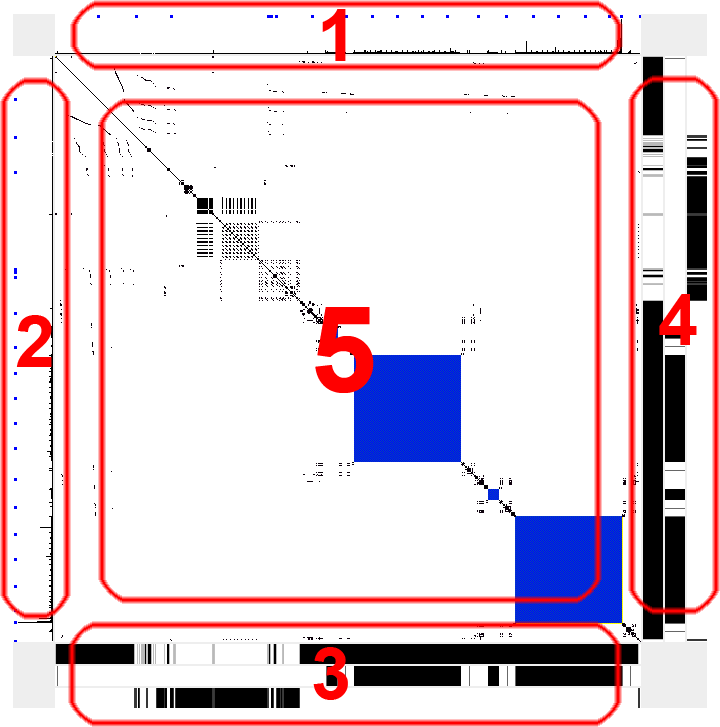
\includegraphics[width=0.4\textwidth]{lviz/elements.png}
\caption{Elements of VDP: axis histograms (Region 1,2);
barcodes (3,4); and extended DotPlot (5). This figure is same as
Figure~\ref{fig:cp-xcopy} with the added annotation.}
\label{fig:elements}
\end{center}
\end{figure}

Here, we develop a novel DotPlot based visualization which is
extensible and can be configured for many uses.
Our visualization, which we call {\em VDP},
consists of a number of sub-visualizations:
an {\em extended DotPlot} (or simply, DP in the rest of the section), two
Axis Histograms, and some barcodes.
% We now describe the elements of VDP.
Figure~\ref{fig:elements} gives an overview of all the elements:
$(i)$ the DP (region 5);
$(ii)$ the x-axis histogram (region 1) and
y-axis histogram (region 2);
and $(iii)$ the x-axis barcodes (region 3) and
y-axis barcodes (region 4).
A larger diagram of the same visualization highlighting various
details is in Figure~\ref{fig:cp-xcopy}.

An important aspect of the VDP is that it is intended to
be extensively customizable. Thus, it gives rise to a family of visualizations.
In Section~\ref{sec:lviz-study}, we show how to apply and customize
the VDP for different purposes. The elements of a VDP as follows.

{\bf DP}:
% We overload the DotPlot (DP) to refer either to our
% entire DotPlot visualization or to the extended DotPlot graphic.
Our DP visualization extends a binary DotPlot in a number of ways.
Since a trace can be long, several events are aggregated
together into a single pixel in a window.
DotPlots which contains aggregated events are drawn as grayscale images
which are then colored using the DP coloring rules for customizing
the appearance.
Normalization or histogram equalization (see Section~\ref{sec:lviz-imp})
is applied on the image so that the color intensity fits in a displayable range.
Our extended DotPlots (see region 5 in the center of Figure~\ref{fig:elements})
can be drawn with event-ordering, time-ordering or time-duration-ordering.
In an {\em event-ordered} DP, the events are plotted in
sequence as they occur in the trace.
In a {\em time-ordered} DP, the events are plotted in time order
according to the start time of the event.
Furthermore, each pixel in the visualization can contain several events
as there may be many events occurring close to each other.
% in start time.
Time-ordering differs from event-ordering in that it can be sparse
and allows empty gap if there are no events in a particular time interval.
Furthermore, in event-ordering,
the number of events in a pixel is constant, whereas
in time-ordering,
some pixels do not contain any event while other pixels may have many events.
In a time-duration-ordered DotPlot, the events are plotted in a similar way
to time-ordering
except that the events will be plotted as a rectangular region
with dimensions corresponding to its duration obtained from
the corresponding events on each axis.
Time-ordering, on the other hand, plots
an event as a single dot.

{\bf DP Matching Rules}:
Unlike a binary DP, our extended DP can look quite different depending
on how matching and coloring rules are specified.
The DP matching rule specifies whether two events
match. The specification allows for matching on
the properties of an event, e.g. PID/TID, program name,
operation type, etc. (see Section~\ref{sec:systrace})
It essentially allows any combination of information about
the event in the trace.
For example, matching based on {\it program name + operation type + resource name}
will give a different visualization from just matching on resource name alone.

{\bf DP Coloring Rules}:
The DP matching rule is used for defining how a DP matches
an event. Given an event which matches the DP matching rule,
the DP color rule specifies what color to display for that event.
% A DP color rule is applicable if the regular expression in the rule
% matches the event.
There can be multiple DP color rules, we use the first matching
rule and there is also a default color if no earlier rules match.
A binary DotPlot, on the other hand, is only in monochrome.

The visualization can be further customized by specifying the colors so
as to combine multiple colors taking
into account either RGB or CMY color modes.
This gives flexibility to emphasize or hide any kind of information
in the trace.
For example, in the RGB mode, the DP color rules
can specify that events which are
file operations are colored red,
registry operations to be blue, and network operations to be green.
Note that the DP color rule matches independently of the DP matching rule,
e.g. the DP match can be on operation type while the DP color rule could be
on program name.

When combining colors, it is easier to use a RGB mode which is
more intuitive. However, in the thesis, CMY is used on all figures.
One way is to use CMY as 3 orthogonal dimensions which would allow 3 different
properties to be visualized.
For example, a cyan pixel in a DP could mean
the events all have property A and an adjacent magenta pixel
would be a different property B.
Intersection or union of properties, e.g. property A and B,
allows cyan and magenta to combine giving blue.
Another way is to simply color properties using custom colors.
Our examples mainly use the first method.

{\bf Barcodes} and {\bf Barcode Coloring Rules}:
The barcode sub-visualization acts as a one-dimensional ruler for the trace on
the associated axis, hence its name.
It visualizes characteristics of events in a single trace.
Region 3 and 4 in Figure~\ref{fig:elements} show X and Y axis barcodes.
The purpose of the barcodes is to visualize multiple aspects of
the trace and allow that to be correlated to the associated event in the DP.

Barcodes are colored using
barcode coloring rules similar to DP coloring rules.
For example Figure~\ref{fig:cp-xcopy} (see Section~\ref{sec:cp})
colors the barcode by resource type.
Multiple barcode coloring rules can be specified.
Since barcodes are useful to show properties of the events,
there can be more than one barcode. Each barcode has its own
set of coloring rules, (see Figure~\ref{fig:cp-xcopy}) which has 3 different
barcodes stacked on the X and Y axis.
In the thesis, we number the barcode from inside (top or left depending
on the axis) to outside, i.e. barcode 1 means the inner most barcode.

{\bf Axis Histograms}:
The axis histogram sub-visualization
serves as another kind of ruler for each of the traces on the X and Y axis,
see region 1 and 2 in Figure~\ref{fig:elements}, providing
time-event correlation information to the traces.
It consists of
ticks (small blue square on the outer edge) representing unit time intervals
and an associated histogram.
Ticks are evenly distributed in a time-ordered or time-duration-ordered VDP
but can be irregularly distributed in an event-ordered VDP,
since there may be many or few events within a unit time interval.
Closely spaced ticks in an event-ordered VDP mean low event frequency.

The histogram component (see region 1 in Figure~\ref{fig:cp-xcopy})
is used to visualize the density of events or time
of the trace.
The histogram in a time-ordered or time-duration VDP
represents the number of aggregated events.
In an event-ordered VDP,
it represents the total time taken (recall that an event has start and end
time) on the aggregated events.

\subsubsection{A VDP Example}

\begin{figure}[htb]
\begin{center}
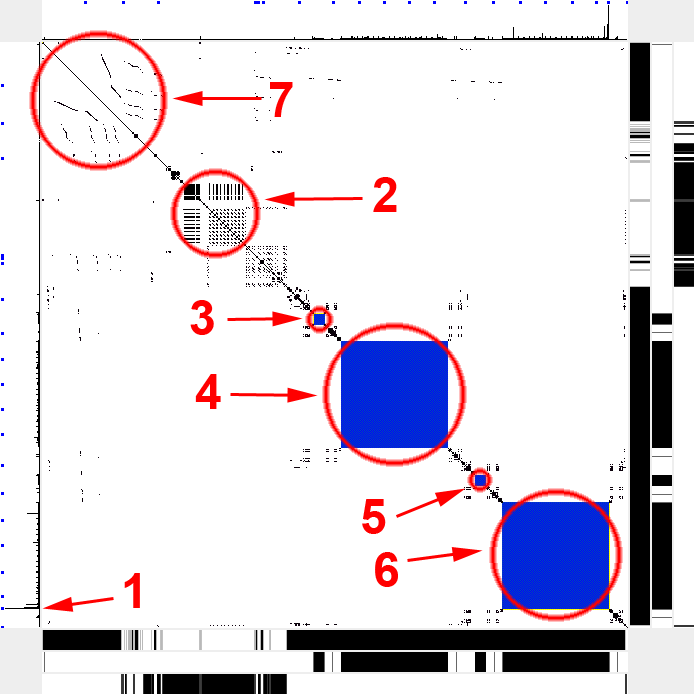
\includegraphics[width=0.5\textwidth]{lviz/cp-xcopy.png}
\caption{Self-comparison event-ordered VDP of {\tt xcopy}
copying 8 files of different sizes with the following configuration rules:
}
\begin{tabular}{ll}
DP match : & operation + parameter (pathname)\\
DP color : & magenta $\rightarrow$ source; cyan $\rightarrow$ destination;\\
 & black $\rightarrow$ other\\
Bar1 color : & black $\rightarrow$ file operation\\
Bar2 color : & black $\rightarrow$ source/destination files\\
Bar3 color : & black $\rightarrow$ registry operation
\end{tabular}
\label{fig:cp-xcopy}
\end{center}
\end{figure}


% \TODO{reviewer 2:
% Move figure 4 closer to the text where it is explained (section 3.3) Actually
% this section is hardly informative. It uses a lot of forward references so I
% have to jump all across the paper to see what it really tries to say. I think
% this section could be skipped since it does not bring additional value in the
% discussion at this point.
% }

Figure~\ref{fig:cp-xcopy} illustrates the event-ordered VDP
of a trace of running
{\tt xcopy} to copy two directories with files of different sizes.
The VDP uses self-comparison of the {\tt xcopy} trace with
the DP matching rule on operation and parameter (resource pathname).
The VDP configuration consisting of a DP ordering, DP matching rule,
DP coloring rules and barcode coloring rules
is given in the caption of the figure.
The non-white regions inside the DP show when {\tt xcopy} is using the
same resource with the same operation and parameter.
Its color represents the resource.
Each blue square is the aggregated visualization effect from
copying a file (see Section~\ref{sec:cp}).
The file sizes are apparent from the sizes of the small (region 3 and 5)
and big (region 4 and 6) blue squares.
We can see that file operations are performed at the start (barcode 1),
but those files are neither source nor destination files (barcode 2).
Registry operations are performed relatively
quickly compared to file operations,
because the blue ticks in the histogram above region 2 are spaced further apart
than the blue ticks above region 4 and 6.
Further discussion on this example is in Section~\ref{sec:cp}.

The DP user interface allows exploration of the trace by zooming in
This allows us to see quite different detail from an aggregated view.
We can see the effects of visualizations at different scales,
Figure~\ref{fig:cp-xcopy} shows the aggregate behavior which
is a different picture from the magnified view in
Figure~\ref{fig:cp-zoom} which shows the individual file operations in {\tt xcopy}.
Zooming creates a new window as one may want to see many different
detail levels at the same time. Clicking inside the DP selects
a pixel to give more details of the events aggregated in that pixel. When
the mode is event-ordering, the events displayed are those events contained
in that pixel. Whereas with time-ordering or time-duration-ordering,
the events are those events which intersect in time with the time interval
represented by that pixel.

\begin{figure}[htb]
\begin{center}

\includegraphics[width=0.10\columnwidth]{lviz/cp-zoom.png}
\caption{The alternate zoomed-in view of a blue region in
Figure~\ref{fig:cp-xcopy} showing reading (magenta) and writing (cyan) operations.
}
\label{fig:cp-zoom}
\end{center}
\end{figure}

% {Zoom and Click}.
% Zoom is one of the most important features that we must have.
% The first time the DotPlot is created, it encompases the entire log files
% that may contain hundred of thousands events.
% The pixel shown in this state contains aggregated number of events
% and the color might be seen as the addition of multiple colors.
% Zoom allows us to go deep into a particular region of interest
% and explore the traces in a more fine grained manner.
% Clicking on the DotPlot area will print out the events
% residing in the clicked region which is very helpful in exploration process.
%
%
% We designed our DotPlots UI to implement the above control operations.
% We use an extensive configuration file to specify most of the parameters for the visualization
% and we use command line interface to interact with the UI.
% The static parameters in the configuration file includes:
% list of log files, list of color rules (regex / plain search pattern),
% DotPlot fields selection, DotPlot color rules, Barcode color rules,
% invert color option, gamma correction value, histogram equalization option, etc...

% The command line accepts 4 commands: "dpe" to render a DotPlot Event-Ordering,
% "dpt" is for DotPlot Time-Ordering, "dptd" is for DotPlot Time-Duration-Ordering,
% and "reload" to reload the configuration file.
%
% A UI frame will pop out when one of the "dpe", "dpt", "dptd" command is put.
% The UI looks like \TODO{Figure ?}
%

\subsection{VDP Implementation and Scalability}
\label{sec:lviz-imp}

There are two important challenges in implementing VDP in \code{lviz}.
Firstly, traces are usually much larger than the size of the screen.
The challenge is to be able to still have usable visualizations given that
there will not be sufficient pixels to show every event.
Secondly, rendering a VDP on large traces needs to be sufficiently fast to
meet interactive UI needs (i.e sub-second response).
Finally, our implementation takes advantage of parallelism given
the trend in multi-core processors.
In this section, we describe an effective and efficient implementation
which meets these challenges.

% Third, a ruler and barcode-like stripes for each axis of the DP
% are added to give additional insight about the region of the inner DP.
% as well as caching can help a lot in responsiveness.

% To fit $100K$ events in a small window screen, a pixel often has
% to accommodate more than one event which in turn will determine
% the brightness / intensity of the pixel.
% The intensity of a pixel is determined by how much
% events in that pixel is a match according to DP matching rule
% (ie. match by program name, path, etc...).
% The hash or message digest (ie. MD5) of the matched fields is
% used to speedup the process of matching tests.
% A pixel that has 10 matched events will look brighter than a pixel
% that has 3 matched events.
% This introduces a grayscale color extension to the DP.
% When the number of matched events are too big, sometimes it exceeds
% the threshold of a grayscale color range [0..255].
% To handle this case, we have $gamma$ normalization to adjust
% the brightness of the pixel. First, the intensity
% (the number of matched events) of each pixel is translated
% to a continuous range value between zero and one inclusive.
% Then each value is mapped to an equation $y = x^(1/g)$ where $g$ is the gamma value.
% The resulting value is then translated to a grayscale color range value [0..255].
% This allow us to reveal the low-intensity pixel.
% The difference can be seen in
% \TODO{Figure~\ref{xx} add explanation to the figures on the differences}.
% Another method to reveal the low intensity pixel is through
% histogram equalization \TODO{cite} which allows for areas with lower
% intensity to have a brighter display without affecting the global intensity.

\begin{figure}[tb]
\begin{center}
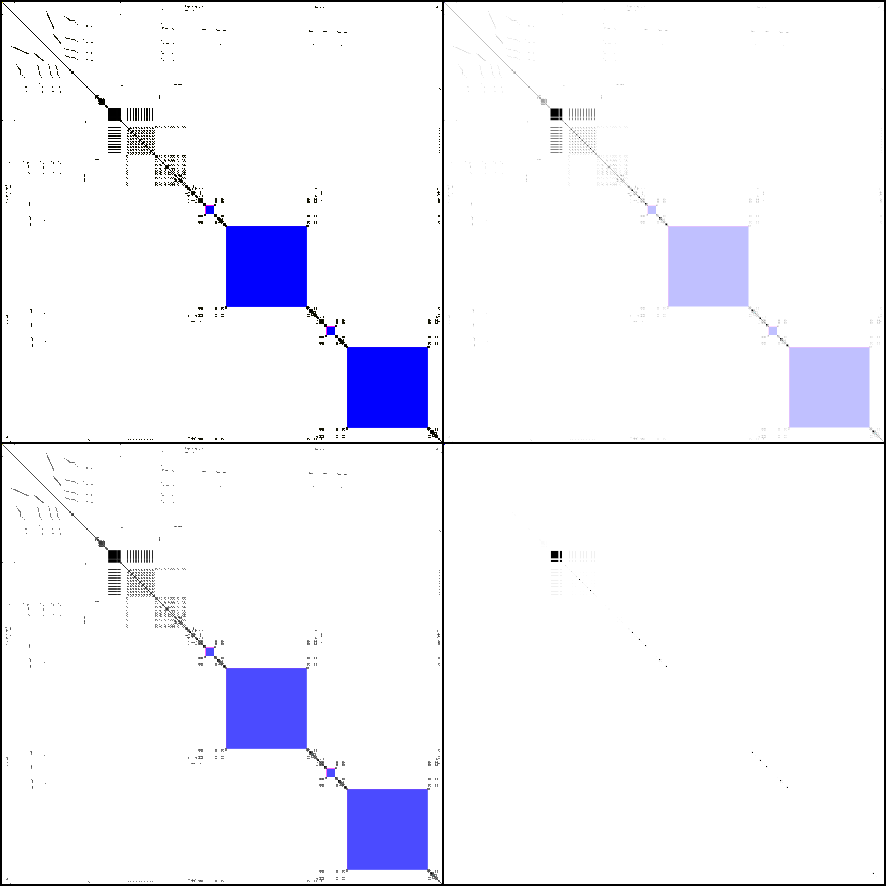
\includegraphics[width=0.5\textwidth]{lviz/gamma.png}
\caption{Clockwise from top-left:
histogram equalization, $\gamma=1$,
$\gamma=1/4$ and $\gamma=4$.
}
\label{fig:gamma}
\end{center}
\end{figure}

Consider a trace with $N$ events and
a display window size with width $W$ and height $H$.
For large traces, e.g. $N=10^6$, clearly $N \gg W$ and $N \gg H$,
and a binary DotPlot with two traces of $N=10^6$ corresponds to an
image with $10^{12}$ pixels (terrapixel).
Our VDP visualization aggregates multiple events into a single pixel,
normalizing it to RGB intensities between $0\ldots255$.
Unlike a digital photo, the intensity of a pixel could be up to $N$,
since aggregating events could end up with all of them
in a single pixel which could easily exceed 255.
\code{lviz} provides two options to deal with this issue by borrowing 
ideas from image processing.
The first is to simply normalize the values.
We extend normalization to include gamma correction, i.e. given an input value $x$,
the output value $y$ is mapped using the equation $y=x^{1/\gamma}$
(pure normalization corresponds to $\gamma = 1.0$).
The second option is histogram equalization which is
a well-known technique in image processing.

% \TODO{reviewer 3:
% The visual scalability discussion in section 4 opens up some serious questions.
% If I understand correctly, what is done is basically aggregation of colors like
% in image processing? This is very dangerous, since a visualization application
% should aggregate the actual data values, or more exactly even, the semantics of
% these values, and not the color mapped values. Just adding up or averaging
% colors can produce meaningless colors or even worse colors which exist in the
% used color map but have another meaning. See for example the work of D. Holten
% et al referred earlier or the work of T. Munzner on accordion drawing,
% guaranteed visibility, and the sequence juxtaposer comparison (available at
% http://www.cs.ubc.ca/~tmm/papers.html)
% }

Figure~\ref{fig:gamma} shows our {\tt xcopy} example visualized
with various normalization options.
In this example with an event-ordered VDP,
the intensity of a pixel shows how many matching events there are in the DP.
We see that histogram equalization (the default) is usually effective
in allowing matching burst events (high intensity) to seen together
with spread out events (low intensity).
While smaller $\gamma$ shows details of the high intensity events,
larger $\gamma$ shows low intensity events.

Most of the cost of rendering a VDP has to do with various forms of
matching: applying DP matching, DP coloring and barcode rules.
We can optimize the rendering to reduce matching costs by pre-processing
the traces. \code{lviz} performs the pre-processing steps when reading the
traces. Subsequent visualizations such as zooming in then make use of
the pre-computed results of the pre-processing phase.

An event in the raw trace is simply a string.
The pre-processing steps involves reducing an event to
a digest value as a more compact representation for DP matching
to operate on and also pre-computing the
results of various coloring rules.
Each event is represented as a hash value which we call a {\em digest}.
The digest helps to speed up event comparisons
as comparing digest values of events is much faster than
the corresponding string comparison, e.g. string matching is slow
as the strings of an event property often have a long common prefix such
as absolute pathname.
The digest of an event is computed based on the DP matching rule that specifies
how to tell if events are considered similar (Section~\ref{sec:lviz-vis}).
For example, if the matching rule is 
{\em program name + operation type + resource name}, the digest
of the event is a hash on those three properties of the event in that order.
We will refer to all the events having the same digest under
the set of DP matching rules as a {\em digest group}.
Thus, the number of digest groups in a trace is equal to the number of distinct hash values.
Note that an event can only belong to one digest group and the hash function
should be good enough to be effectively collision free so that 
two events which do not match (according to the DP matching rule) are
not hashed to the same digest group.

% The DP coloring rules extend the visualization to 24-bit color DP.
% We employ a pre-processing strategy 
% to speedup the matching of color rules (DP and Barcode).
% Once two events are considered a match by the DP matching rule, 
% those events will be colored based on the DP color rules.
It is common that the pattern in a coloring rule only needs a string
match.
Since there can be many color rules, we want to avoid applying
to the matching events one rule at a time.
We instead employ the Aho-Corasick's string matching
algorithm \cite{aho1975efficient}
to compile all the rules (the string patterns) into a single automaton.
This allows us to identify the color in a single pass
rather than multiple passes for each rule.

\begin{algorithm}[htb]
\KwIn{$L_X[0\ldots N-1]$ as log X; and $L_Y[0\ldots N-1]$ as log Y}
\KwOut{2D array $S[0\ldots W-1,0\ldots H-1]$ as pixel intensity}
\BlankLine
zero fill $S$\;
\For{$x\leftarrow 0$ \KwTo $N-1$}{
  \For{$y\leftarrow 0$ \KwTo $N-1$}{
    \If(\tcp*[f]{based on DP matching rule}){$L_X[x]$ matches $L_Y[y]$}{
      $S[xW/N,yH/N] ++$
    }
  }
}
\caption{Naive $O(N^2)$ Algorithm}
\label{alg:lviz-naive}
\end{algorithm}

The two pre-processing steps above are performed once and
cached in memory for later use when rendering the VDP.
The VDP rendering has to be fast as it is
used interactively for real-time browsing 
which entails zooming in on a region within the DP.
As the number of events in a trace, $N$, grows in order of hundreds of thousands,
the naive DP Algorithm~\ref{alg:lviz-naive}
takes $O(N^2)$ becomes infeasible.
To simplify our illustration, we assume both logs have the same number
of events.
We developed a new DP rendering algorithm which scales well to large traces.

\begin{algorithm}[htb]
\KwIn{$L_X[0\ldots N-1]$ as log X; and $L_Y[0\ldots N-1]$ as log Y}
\KwOut{Associative array $D_X[d]$ whose key $d$ is the digest of an event
and value is a set of integers representing indexes of events in $L_X$ whose
digests are $d$. Similarly for $D_Y[d]$.}
\BlankLine
\For{$x\leftarrow 0$ \KwTo $N-1$}{
  $d\leftarrow digest(L_X[x])$ \tcc*[l]{digest() calculates the digest based on the DP matching rule}
  insert x to the set $D_X[d]$
}
\For{$y\leftarrow 0$ \KwTo $N-1$}{
  $d\leftarrow digest(L_Y[y])$\;
  insert y to the set $D_Y[d]$
}
\caption{Preprocessing step to get digest group}
\label{alg:lviz-algpre}
\end{algorithm}

\begin{algorithm}[htb]
\KwIn{$D_X[d]$ and $D_Y[d]$ from Algorithm~\ref{alg:lviz-algpre}}
\KwOut{2D array $S[0\ldots W-1,0\ldots H-1]$ as pixel intensity}
\BlankLine
zero fill $S$\;
\ForEach{digest $d$}{
  \ForEach{$x$ in $D_X[d]$}{
    \ForEach{$y$ in $D_Y[d]$}{
      $S[xW/N,yH/N] ++$
    }
  }
}
\caption{New algorithm for large screen size}
\label{alg:lviz-alg1}
\end{algorithm}

The core of new DP rendering algorithm is based on two observations.
The first observation is that for each matching event,
a certain intensity value can be added incrementally.
Two events are considered a match if they are in the same digest group.
Events in different digest groups will never match thus will never be rendered.
The incremental algorithm effectively processes only the events
that contribute to the visualization and prunes all other events.
Consider digest group $D_i$ which has $S_i$ events.
It can be processed in time $O(S_i^2)$
and the result for this digest group can be added incrementally to the 
end result.
This significantly reduces the number of matching comparisons needed
from $O(N^2)$ down to $\sum_{i=1}^{G} S_i^2$
where $G$ is the number of digest groups in the trace.
Algorithm~\ref{alg:lviz-algpre} pre-process the two logs $L_X$ and $L_Y$
into digest groups stored in associative arrays $D_X$ and $D_Y$.
This preprocessing step takes $O(N)$ time and is executed only once.
Algorithm~\ref{alg:lviz-alg1} iterates each digest group and accumulates
the number of matches.

\begin{algorithm}[htb]
\KwIn{$D_X[d]$ and $D_Y[d]$ from Algorithm~\ref{alg:lviz-algpre}}
\KwOut{2D array $S[0\ldots W-1,0\ldots H-1]$ as pixel intensity}
\BlankLine
zero fill $S$\;
\ForEach{digest $d$}{
  declare temporary integer array $S_X[0\ldots W-1]$ and $S_Y[0\ldots H-1]$\;
  zero fill $S_X$ and $S_Y$\;
  \lForEach{$x$ in $D_X[d]$}{
    $S_X[xW/N] ++$
  }\;
  \lForEach{$y$ in $D_Y[d]$}{
    $S_Y[yH/N] ++$
  }\;
  \For{$w\leftarrow 0$ \KwTo $W-1$}{
    \For{$h\leftarrow 0$ \KwTo $H-1$}{
      $S[w,h]\leftarrow S[w,h]+S_X[w]\times S_Y[h]$
    }
  }
}
\caption{New algorithm for small screen size}
\label{alg:lviz-alg2}
\end{algorithm}

However, in the worst case, a digest group $S_i$ can be as large as $N$.
This drawback leads us to the second observation which
gives an optimization for the case when the digest group size is large.
It exploits the fact that $N > W\times H$ and often also $N \gg W\times H$.
Consider a digest group with $S_i$ events.
The intensity (color) for each event in that group can be recorded as
its projection on the X and Y axis of the window.
This is easily done by keeping track of the color intensities in
two arrays with size $W$ and $H$ respectively in $O(S_i)$ time.
Therefore, the resulting DP on a window of size $W \times H$
can be drawn based on the projected intensities in $O(S_i + W\times H)$ time,
as shown in Algorithm~\ref{alg:lviz-alg2}.

\begin{algorithm}[htb]
\KwIn{$D_X[d]$ and $D_Y[d]$ from Algorithm~\ref{alg:lviz-algpre}}
\KwOut{2D array $S[0\ldots W-1,0\ldots H-1]$ as pixel intensity}
\BlankLine
zero fill $S$\;
\ForEach{digest $d$}{
  \nlset{$\alpha$} \eIf{$|D_X[d]|\times |D_Y[d]|<|D_X[d]|+|D_Y[d]|+W\times H$}{
    \ForEach{$x$ in $D_X[d]$}{
      \ForEach{$y$ in $D_Y[d]$}{
        $S[xW/N,yH/N] ++$
      }
    }
  }{
    declare temporary integer array $S_X[0\ldots W-1]$ and $S_Y[0\ldots H-1]$\;
    zero fill $S_X$ and $S_Y$\;
    \lForEach{$x$ in $D_X[d]$}{
      $S_X[xW/N] ++$
    }\;
    \lForEach{$y$ in $D_Y[d]$}{
      $S_Y[yH/N] ++$
    }\;
    \For{$x\leftarrow 0$ \KwTo $W-1$}{
      \For{$y\leftarrow 0$ \KwTo $H-1$}{
        $S[x,y]\leftarrow S[x,y]+S_X[x]\times S_Y[y]$
      }
    }
  }
}
\caption{Combined algorithm from \ref{alg:lviz-alg1} and \ref{alg:lviz-alg2}.
(Line $\alpha$ can be further tuned with some constant factors)}
\label{alg:lviz-alg3}
\end{algorithm}

Both algorithms can be combined together to
get the best of both worlds, which gives
a DP rendering time complexity of $\sum_{i=1}^{G} min(S_i^2, S_i + W\times H)$,
as shown in Algorithm~\ref{alg:lviz-alg3}.
That is, for each digest group $S_i$ that satisfies $S_i^2 < S_i+W\times H$, 
the $O(S_i^2)$ algorithm is used;
otherwise, the $O(S_i + W\times H)$ algorithm is used to obtain a sub-image.
Adding the intensities of all the sub-images of all digest groups gives the final image.

We illustrate the complexity of the algorithm to process $N=10^6$ events.
The worst case is when the number of digest groups $G$ is $10^3$
and each digest group has size $10^3$.
Suppose the window screen size is $1000\times 1000$.
Then the first $O(S^2)$ algorithm is used giving $GS^2 = 10^9$ operations.
If the window size is resized to $600\times 400$, then
the second $O(S+W\times H)$ algorithm is used giving $G(S+WH)=2.41\times 10^8$ operations.
This is much faster than the naive algorithm which would take $O(10^{12})$
operations.
The best case is achieved when each digest group only contains one event.
This means $G = 10^6$ and the number of operations
is $G S^2=10^6$.
Another good case is when there is only one digest group,
so $S=10^6$ and the number of operations is $G(S + W\times H)=1.24\times10^6$.

\code{lviz} is multi-threaded to make use of multi-core processors.
The pre-processing steps and rendering algorithms can be easily parallelized.
The events in the trace can be split up into several sub-traces and 
the pre-processing can be applied to each sub-trace
independently and in parallel.
We implemented and tested the rendering algorithm using
OpenJDK 1.6.0\_18 (64bit) on an Intel Core i7-960 3.20GHz
machine with 12G RAM.
An uncompressed 120MB trace file with 558K events took 2.8 seconds
to read and finish the two pre-processing steps using 8 threads.
To see the effectiveness of parallel pre-processing, it took 6.0 seconds,
when the execution is single-threaded.
In our rendering algorithm, each digest group can be processed
independently and in parallel as there is no dependency between digest groups.
We also render all the sub-components
of a VDP, the DP, barcodes, and histograms in parallel.
It took about 0.5 seconds to render the trace where the DP has 550K events
on both axis.
Thus, \code{lviz} can process large traces with sufficient real-time response
when the user interactively zooms/resizes the VDP or changes the histogram.

To speed up subsequent runs, \code{lviz} creates a cache containing the results
of the pre-computations of the digest, DP color, barcodes color
of each event since they require the most computation
and are the bottleneck of the system. The cache avoids recalculating the
digest and the coloring rules every time the program is run.
This cache is rebuilt if the corresponding rules change.
Loading from the cache skips the pre-computation steps and
cuts down the trace loading time to 1.3 seconds.
The speedup is more significant when the matching and coloring rules are
more complicated.

% \TODO{reviewer 2:
% The scalability solution seems, from what I can read, well thought. However I
% wonder if a comparatively fast result, if not a faster one, could not have been
% obtained, with less programming effort, by using a pixel shaders or CUDA
% implementation.
% }

% While the DP treats each event independently,
% RTG has to show the connections
% between events for visualizing the resource life cycle.
% If we consider each event as an operation on a resource
% (e.g. file or registry key),
% each resource is associated with a sequence of operations which includes
% creating a new one, opening an existing one, reading, writing/modifying, closing, deletion.
% If we further assume the resource life cycle has three states:
% non-existence, exists but not
% opened, opened, we can use the sequence of operations to
% reconstruct the state transitions for RTG visualization.
% However, there are some exceptions to be noted.
% Firstly, we may be dealing with a trace
% only during some time period, i.e. some
% resource can be opened before logging happens,
% thus we have to ``guess'' the initial state of the resource.
% We employ a heuristic based on the first observed operation of each resource.
% Secondly, file deletion in Windows is done in a special system call
% {\tt NtSetInformationFile} which puts file into ``delete after close'' state.
% In order to delete a file, one should first open the file,
% then call {\tt NtSetInformationFile} to set the ``delete after close'' state,
% finally close the file and if no other processes are opening the file, it will
% be deleted.
% Lastly, there is an additional rename operation
% which is translated in our RTG as a combination
% of deletion and creation operations.

\section{Case Studies}
\label{sec:study}

The following case studies show how \lviz{} can be used to
understand system behavior and to solve system or application problems.
We first use a well understood task, file copying,
to familiarise the reader with \VDP{}.
We then use a software compilation example to show how \VDP{} can
be used for software failure diagnosis.
We use two visualizations on whole system traces to understand
how the operating system works and examine performance problems.
Lastly, we use \VDP{} to examine performance problems in a browser benchmark.
These examples also illustrate that the \VDP{} visualization is highly
customizable and in practice, one could use many different visualizations
on the same trace.

% In order to demonstrate the potential and power of visualizing system traces,
% we have developed a visualization tool \VDP{} using an extension of
% dotplots \cite{dnadp}.
% Dotplots were used to show sequence similarity in
% DNA \cite{dnadp} and music \cite{audio}.
% Our \VDP{} dotplots (or simply \VDP{} for both the visualization and tool)
% extends the basic dotplot to get a flexible visualization
% which can be tailored to visualize different kinds of behavior.
% Furthermore, \VDP{} uses a number of novel extensions geared towards
% understanding software behavior whereas traditional uses of dotplots
% are for showing sequence similarity.

The notation Bar $n$ refers to the $n$th barcode.
The configuration of each visualization is described in the corresponding
figure caption.

\subsubsection{Comparing File Copying Programs}
\label{sec:cp}

% \TODO{problems to solve: 1. finding repeated patterns
% 2. diagnose performance problem (8k buffer)}

% \begin{figure}[htb]
% \begin{center}
% 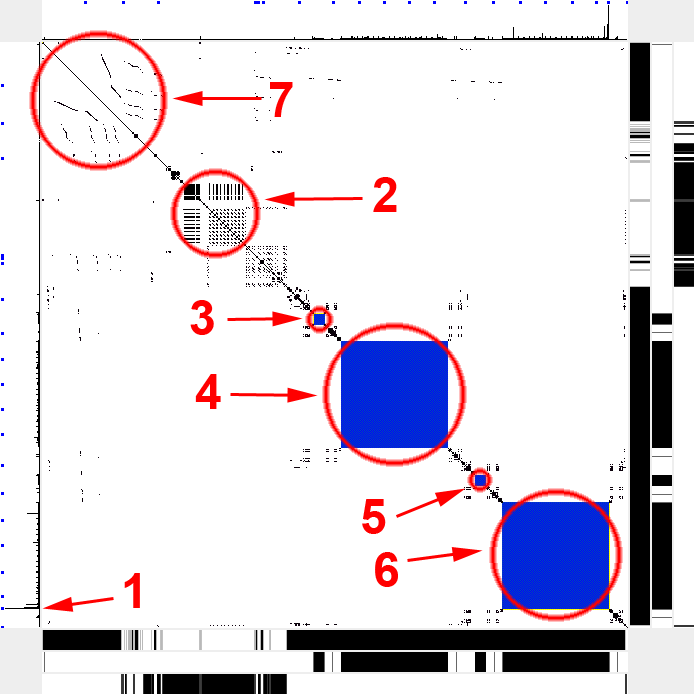
\includegraphics[width=1.0\columnwidth]{lviz/cp-xcopy.png}
% \caption{Self-comparison event-ordered \VDP{} of {\tt xcopy}
% copying 8 files of different sizes with the following configuration rules: 
% }
% \begin{tabular}{ll}
% DP match : & operation + parameter (pathname)\\
% DP color : & magenta $\rightarrow$ source; cyan $\rightarrow$ destination;\\
%  & black $\rightarrow$ other\\
% Bar1 color : & black $\rightarrow$ file operation\\
% Bar2 color : & black $\rightarrow$ source/destination files\\
% Bar3 color : & black $\rightarrow$ registry operation
% \end{tabular}
% \label{fig:cp-xcopy}
% \end{center}
% \end{figure}

\begin{figure}[htb]
\begin{center}

\includegraphics[width=0.10\columnwidth]{lviz/cp-zoom.png}
\caption{The alternate zoomed-in view of a blue region in
Fig.~\ref{fig:cp-xcopy} showing reading (magenta) and writing (cyan) operations.
}
\label{fig:cp-zoom}
\end{center}
\end{figure}

We use an example of a simple program and operation,
namely, file copying using \xcopy{}, to explain various
aspects of the \VDP{} visualization.
Fig.~\ref{fig:cp-xcopy} shows a self-comparison event-ordered \VDP{} of
\xcopy{} copying 8 files with sizes
1MB, 10KB, 10MB, 100KB, 1MB, 10KB, 10MB and 100KB and in that given order.
A self-comparison \VDP{} has a 45$^\circ$ diagonal line from top-left to 
bottom-right corner because events on the diagonal always match.
The structure of the files being copied is visible as blue squares in
Region {\em 3}, {\em 4}, {\em 5} and {\em 6} which show copying the
first 1MB and 10MB, then the second 1MB and 10MB files.
It is interesting to see the effect of scale on the visualization.
At this scale, which shows everything, the relative file sizes are also
visible for the large files.  The smaller 10KB and 100KB files are 
too small to be seen at this scale but are visible when zoomed in.
By correlating Bar1 and Bar2,
we find that there are some file related operations in the early phase,
but those files are neither source nor destination files of \xcopy{}.
This might seem surprising. To answer that question, we
click on Region 7, which shows that
the files in question are DLLs. Thus, the top-left region 
shows \xcopy{} loading DLLs.

Bar3 shows that Region {\em 2} has many registry operations which might
be surprising for a file copying task.
% This shows that a command line program can also have many
% registry operations.
The histogram spike at Region 1 shows that some events at the end of the
trace take a long time.
Fig.~\ref{fig:cp-zoom} is a zoomed-in view to one of the blue squares in
Fig.~\ref{fig:cp-xcopy}.
The checkerboard-like pattern shows alternating read (magenta) and write
(cyan) operations which is what we expect for file copy.
Since $cyan+magenta=blue$,
this explains that the blue squares in Fig.~\ref{fig:cp-xcopy} represents
reading from source files and writing to destination files.
We see also that visualizations at different scales can be used for
different purposes.
The extreme magnification in Fig.~\ref{fig:cp-zoom}
shows the actual operations but may be too detailed a view for
the overall picture which emerges at the other extreme in 
Fig.~\ref{fig:cp-xcopy}.

\begin{figure}[tbh]
\begin{center}
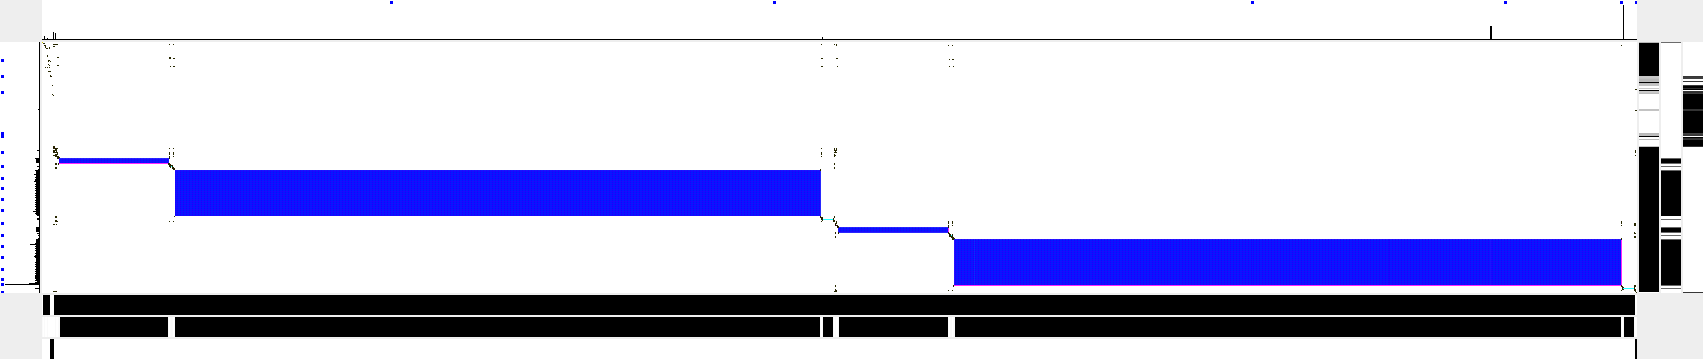
\includegraphics[width=1.0\columnwidth]{lviz/cp-xvc.png}
\caption{Event-ordered \VDP{} comparing {\tt cp} (x-axis) and {\tt xcopy} (y-axis) copying
the same files. 
The configurations are the same as in Fig.~\ref{fig:cp-xcopy}.
}
\label{fig:cp-xvc}
\end{center}
\end{figure}
%
\begin{figure}[htb]
\begin{center}
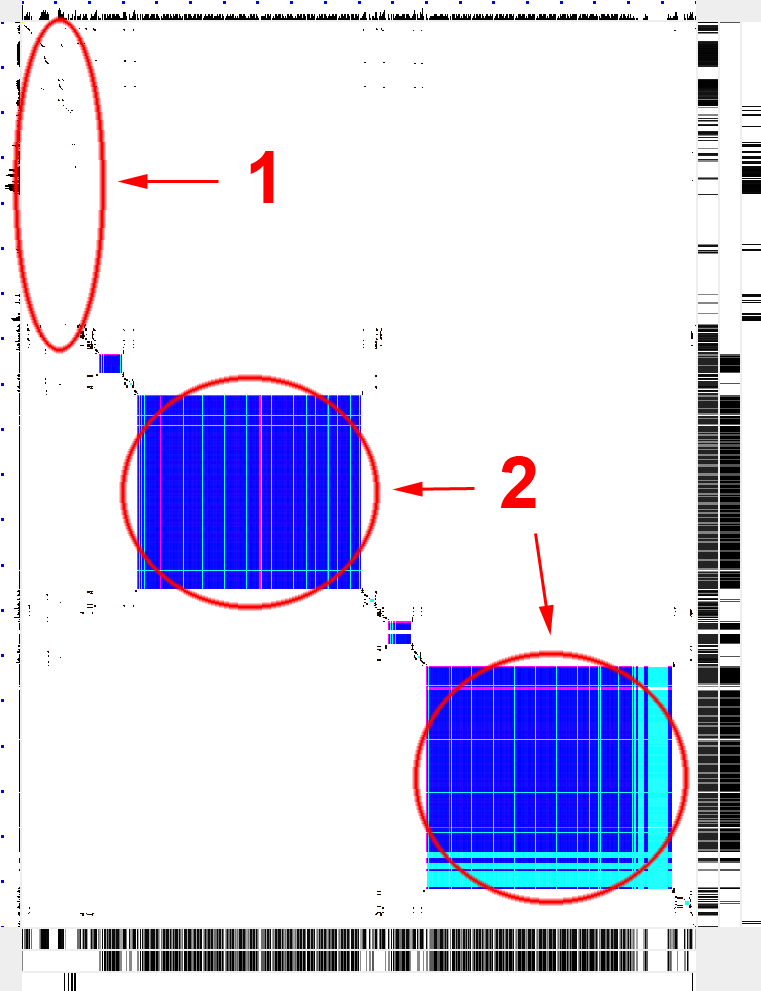
\includegraphics[width=0.6\columnwidth]{lviz/cp-64k.png}
\caption{Time-ordered \VDP{} comparing {\tt cp-64k} (x-axis)
and {\tt xcopy} (y-axis).
The configurations are the same as in Fig.~\ref{fig:cp-xcopy}.
}
\label{fig:cp-64k}
\end{center}
\end{figure}

In general, a \VDP{} is used with two traces rather than a single
trace as in a self-\VDP{}.
% Fig. \ref{fig:cp-xcopy} shows a \VDP{} which compares of a {\tt xcopy}
% trace against itself, i.e. a self-similarity comparison.
% Two different traces can also be compared with one trace on the X axis
% and the other trace on the y-axis.
Fig.~\ref{fig:cp-xvc} compares {\tt cp} (x-axis: a Windows version
of GNU {\tt cp}) and {\tt xcopy} (y-axis) copying the same 8 files.
% {\tt cp} is the Windows version of the file copying program included
% in GNU coreutils.
The \VDP{} is much wider than its height, giving
wide blue rectangles instead of blue squares 
(Fig.~\ref{fig:cp-xvc} versus Fig.~\ref{fig:cp-xcopy}).
% \TODO{double check width:height, shouldnt it be 16x?}
% Measuring the width and height of the rectangle,
% we find the ratio of width to height is approximately ? times.
Thus, {\tt cp} performs many more operations than {\tt xcopy}.
To investigate further, zooming in and examining individual events, 
we find that each read and write operation uses a buffer size of 4K,
while {\tt xcopy} uses 64K.
This means that {\tt cp} has 16 times more read and write operations
than {\tt xcopy}.
This is consistent with the width-height ratio in the visualization.

% \begin{figure}[htb]
% \begin{center}
% \includegraphics[width=1.0\columnwidth]{cp-xvct.png}
% \caption{Same as Fig.~\ref{fig:cp-xvc} but the axises are in time units.}
% \label{fig:cp-xvct}
% \end{center}
% \end{figure}

In order to compare the performance of {\tt cp} and {\tt xcopy},
we can use a time-ordered \VDP{}.
% In time based \VDP{}, events are distributed on the axises based on their
% relative time to the first event, while in event based \VDP{}
% events are distributed uniformaly.
Changing the visualization to a time-ordered one (not shown)
shows that {\tt cp} runs slower than {\tt xcopy} though less than 16x.
We then modified {\tt cp} to obtain another version
{\tt cp-64k} which uses 64K buffers.
Fig.~\ref{fig:cp-64k} shows the time-ordered \VDP{} comparing
{\tt cp-64k} (x-axis) and {\tt xcopy} (y-axis).
From Region {\em 2}, we can see that copying of the largest file
is performed in about the same time in both programs.
However, {\tt xcopy} has a slow initialization 
(as shown in Fig.~\ref{fig:cp-64k} Region {\em 1} which includes the registry
operations in Fig.~\ref{fig:cp-xcopy} Region {\em 2}),
which causes {\tt xcopy} to be slower in total than {\tt cp-64k}.

% \TODO{discuss flexible configuration and exploration process also shown
% in the other case studies}



\subsubsection{A Software Build Case Study}
\label{sec:build}

\begin{figure}[htb]
\begin{center}
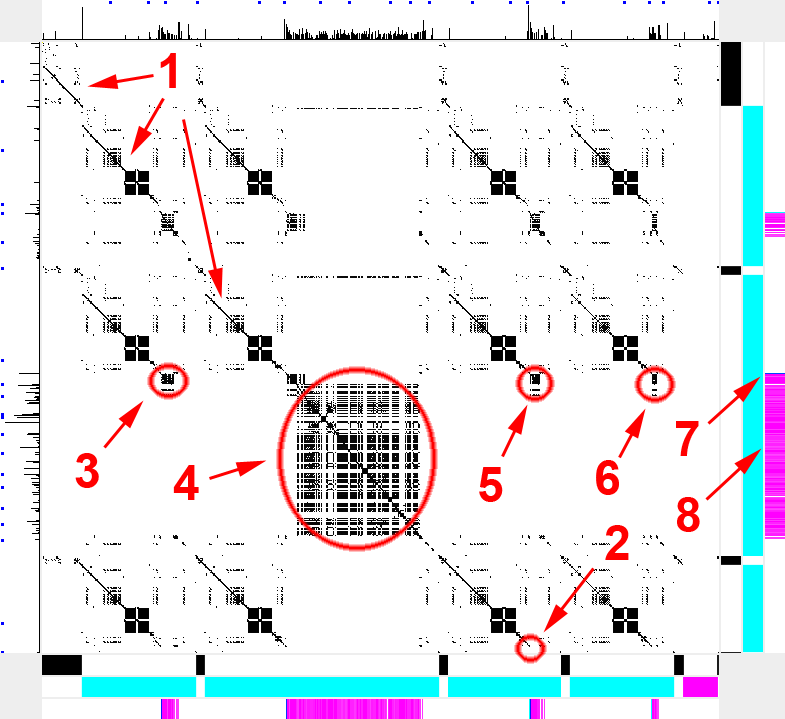
\includegraphics[width=1.0\columnwidth]{lviz/make-fail.png}
\caption{Event-ordered \VDP{} comparing a successful (x-axis)
software build process and a failed (y-axis) one.
%DP matching: program, operation and value (pathname);
%DP color: any=black;
%Bar1: {\tt nmake.exe}=black;
%Bar2: {\tt cl.exe}=cyan, {\tt link.exe}=magenta;
%Bar3: reading {\tt .c}/{\tt .h} files = cyan/magenta.
\label{fig:make-fail}
}
\begin{tabular}{ll}
DP match : & program + operation + value (pathname)\\
DP color : & black $\rightarrow$ any\\
Bar1 color : & black $\rightarrow$ {\tt nmake.exe}\\
Bar2 color : & cyan $\rightarrow$ {\tt cl.exe}; magenta $\rightarrow$ {\tt link.exe}\\
Bar3 color : & cyan $\rightarrow$ reading {\tt .c} files;\\
 & magenta $\rightarrow$ reading {\tt .h} files
\end{tabular}
\end{center}
\end{figure}

\begin{figure*}[htb]
\begin{center}
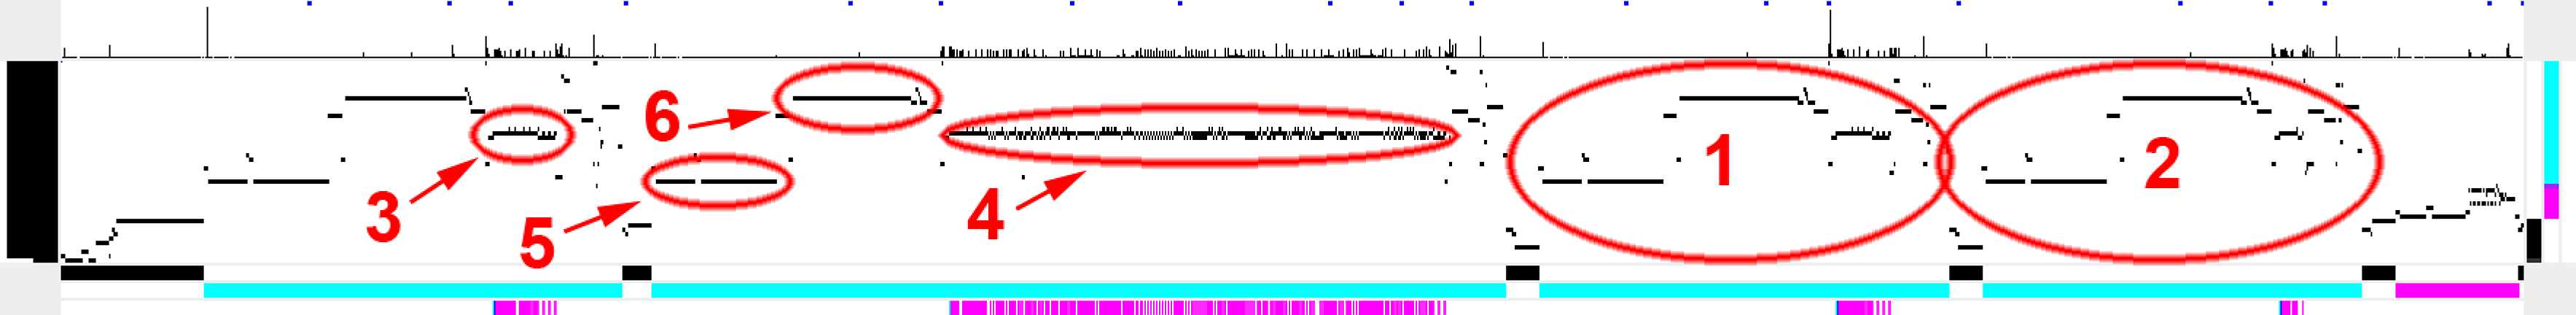
\includegraphics[width=1.0\textwidth]{lviz/make-pp.png}
\caption{Program point event-ordered \VDP{} of project build: pseudo program point trace (y-axis).
}
DP match: program name + program point;
DP color: black $\rightarrow$ any;
Barcode coloring rules are the same as in Fig.~\ref{fig:make-fail};
Bar3 in y-axis is undefined as the pseudo trace does not have operation type.
\label{fig:make-pp}
\end{center}
\end{figure*}

We now apply visualization to diagnose program failure.
In Fig.~\ref{fig:make-fail}, we compare a successful software project build
with a failed one to explain the failure.
The project consists of 4 C files, a header file and a {\tt makefile}.
We use {\tt nmake.exe} from Visual Studio to build the project.
To deliberately cause failure, one of the C files is changed
to be unreadable.

% Before identifying the cause of the failure,
We first explain what the visualization shows.
From the Bar2 of x-axis, 
we can see 4 {\tt cl.exe} processes (4 cyan regions), which tallies
with the number of C files.
There is one invocation of {\tt link.exe} (magenta),
occurring at the end of the trace.
By correlating Bar2 and Bar3, we see that
{\tt cl.exe} processes first read a C file (tiny blue bar in region {\em 7})
and then read a number of header files (long magenta bar in region {\em 8}).
Different {\tt cl.exe} processes read a different number of header files,
see sizes of regions {\em 3}, {\em 4}, {\em 5}, {\em 6} differ.

In a self-comparison \VDP{}, there will be a 45$^\circ$
diagonal line from top-left to bottom-right corner.
% The diagonal line means that the events
% on both x-axis and y-axis match (which is obviously true for self-comparison).
Fig.~\ref{fig:make-fail} shows a 45$^\circ$ diagonal (Label {\em 1})
with some breaks, from
the start to region {\em 2}, near the end of the failed build (y-axis).
It shows that the traces are basically similar till the failure point
when the build terminates.
By zooming in (not shown),
we see that the failure occurs at the third invocation of
{\tt cl.exe}, just before reading the C file.
Thus, the \VDP{} shows how file I/O works in the build and we use this
to identify a failed build.
One might argue that the compiler's error message is a better solution.
However, firstly,
not all software give detailed error message like the compiler in this case.
Secondly, due to software bugs, the error message could be wrong, while 
the system trace reports the actual underlying issues.

The build example is reused to show a visualization of the code structure
of {\tt cl.exe} in Fig.~\ref{fig:make-pp}.
We use a pseudo trace (y-axis) consisting of the program name
concatenated with its program point in the binary (an instruction address)
which is sorted by program name and address.
The program point comes from the stack walk corresponding to the event
and corresponds to the latest return address in the stack trace
coming from the executable or earliest DLL.
The x-axis trace is as before in Fig.~\ref{fig:make-fail}.

Region {\em 1} and {\em 2} show two invocations of {\tt cl.exe}
having similar patterns.
In fact, all 4 invocations follow the same pattern which can be broken
up into three main components:
region {\em 5}, {\em 6} and {\em 4}.
By zooming in and looking at the events, we infer that
region {\em 5} and {\em 6} is in the initialization phase of the compiler, which include
loading of DLL files and reading configurations from the registry.
Region {\em 6} is the reading of a large DLL {\tt rsaenh.dll}.
By looking at Bar3,
region {\em 3} and {\em 4} are the reading of C and header files.
As different C files have different header includes,
region {\em 3} and {\em 4} have different widths.
The fine squiggles in region {\em 3} and {\em 4} represent
three different file operations: open, read and close.
For each header file, there is one file open and close event,
with a differing number of file read operations depending
on the file size.
This makes the squiggles irregular.
Since this \VDP{} is based on program points, it shows directly the 
structure of the function calls. Thus, it visualizes
the code while Fig.~\ref{fig:make-fail} compares the operations
due to system calls.
It is also different from the source code visualization in \cite{tralfamadore}
and we do not need to rely on availability of source code.

The configurations play an important role in a \VDP{}.
Fig.~\ref{fig:make-matching} shows two \VDPs{} 
which are visually different from each other and also Fig.~\ref{fig:make-fail}
but they are all visualizations of the same underlying trace.
The \VDPs{} in Fig.~\ref{fig:make-matching} and 
Fig.~\ref{fig:make-fail} only differ in the DP matching rule and
the rest of the configuration is the same.
% The rest of the configuration and the two traces are exactly the same.
The left side \VDP{} in Fig.~\ref{fig:make-matching} uses only the event 
operation as the DP matching rule.
It can be used to highlight same or different operations.
The right side \VDP{} uses the program name, and can be used to
show different programs used in the project build process.

\begin{figure}[htb]
\begin{center}
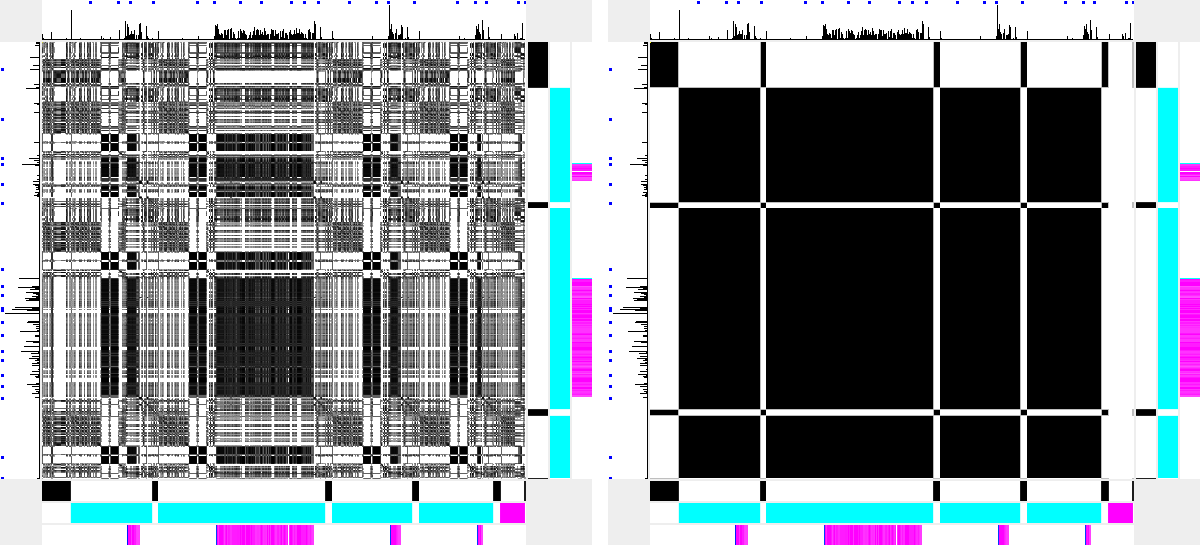
\includegraphics[width=1.0\columnwidth]{lviz/make-matching.png}
\caption{Changing the DP matching rule of Fig.~\ref{fig:make-fail}.
Left side DP matching rule is operation; Right side is program name.
}
\label{fig:make-matching}
\end{center}
\end{figure}

\TODO{reviewer 2:
In the second example, figure 8, a similar question: how do I know that a cyan bar is cl.exe and not some other
process - as a user I mean, not reading the legend of the figure? But the main question I have is why would a user go
to this level of effort to find why a build failed, he can always use the compiler's build log to find much more precisely
and more quickly what happened.
fixed.
}

\subsection{Visualizing Idle System Traces}
\label{sec:idle}

\begin{figure*}[htb]
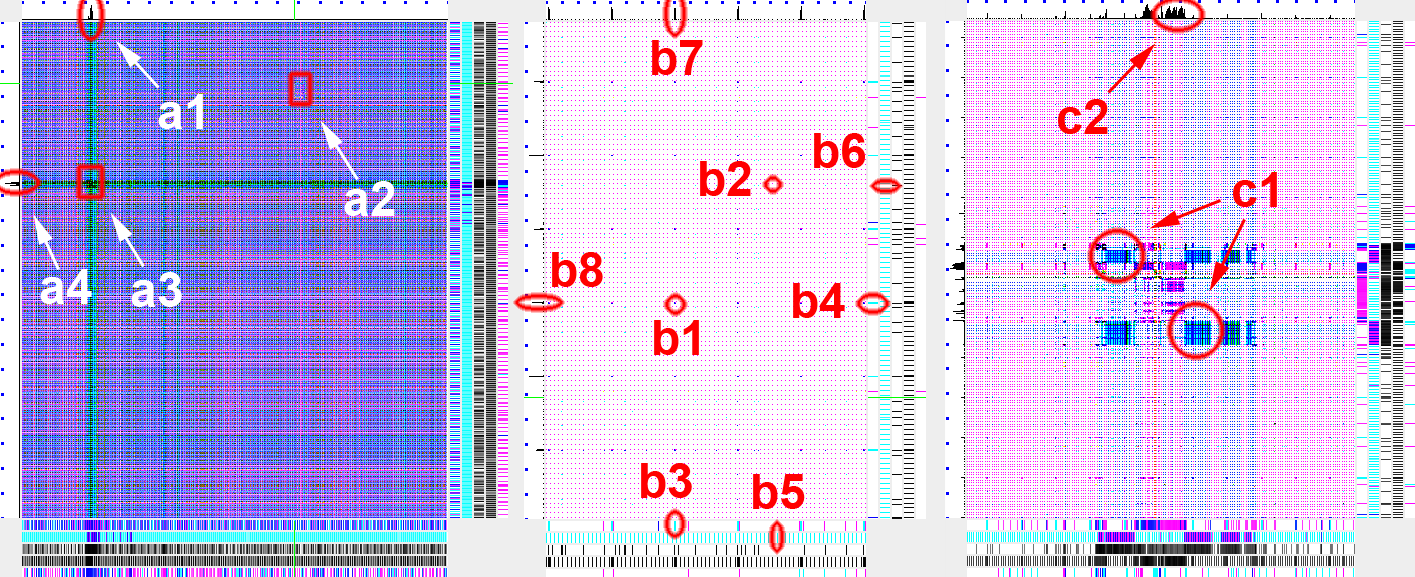
\includegraphics[width=1.0\textwidth]{lviz/idle-dp.png}
\caption{Time-ordered \VDP{} comparing two idle systems.
{\bf a.} (left) comparing one hour interval between two machines;
{\bf b.} (middle) zoom in of Region {\em a2};
{\bf c.} (right) zoom in of {\em a3}.
%DP Matching: (program,operation);
%DP color: file=cyan, registry=magenta, other operation=yellow;
%Bar1: lsass.exe=cyan, svchost.exe=magenta;
%Bar2: explorer.exe=cyan, wuauclt.exe=magenta;
%Bar3: file=black;
%Bar4: registry=black;
%Bar5: network=cyan, process\&thread creation\&termination=magenta.
The different DP color intensity in the zoomed views is caused by
histogram equalization.
}
\label{fig:idle-dp}
% \begin{tabular}{ll}
% DP match : & program + operation\\
% DP color : & cyan $\rightarrow$ file; magenta $\rightarrow$ registry; yellow $\rightarrow$ others\\
% Bar1 color : & cyan $\rightarrow$ lsass.exe; magenta $\rightarrow$ svchost.exe\\
% Bar2 color : & cyan $\rightarrow$ explorer.exe; magenta $\rightarrow$ wuauclt.exe\\
% Bar3 color : & black $\rightarrow$ file\\
% Bar4 color : & black $\rightarrow$ registry\\
% Bar5 color : & cyan $\rightarrow$ network, magenta $\rightarrow$ process \& thread creation \& termination
% \end{tabular}
{\it DP match}: program + operation;
{\it DP color}: cyan $\rightarrow$ file; magenta $\rightarrow$ registry; yellow $\rightarrow$ others;
{\it Bar1 color}: cyan $\rightarrow$ lsass.exe; magenta $\rightarrow$ svchost.exe;
{\it Bar2 color}: cyan $\rightarrow$ explorer.exe; magenta $\rightarrow$ wuauclt.exe;
{\it Bar3 color}: black $\rightarrow$ file;
{\it Bar4 color}: black $\rightarrow$ registry;
{\it Bar5 color}: cyan $\rightarrow$ network, magenta $\rightarrow$ process \& thread creation \& termination.
\end{figure*}


Previous examples compared the trace of particular programs
% against another
% so that we can compare the behavior of the two programs
(or to understand
how a program behaves using a self-similarity \VDP{}).
We now show that visualization can also be useful for system traces
as a whole -- a system trace is the complete trace of the entire operating
system for a period of time.

% \TODO{what is the problem}

When Windows is idle (i.e. no user interaction), 
system services and system processes still run.
We want to visualize whether such services and programs have 
(some expected) periodic behavior.
Fig.~\ref{fig:idle-dp}a (left) shows a time-ordered \VDP{} from two 
different idle machines for an hour at different times.
The size of the x and y-axis traces are 
851528 and 652713 events respectively.
% \footnote{
% Our \VDP{} tool handles large traces with real-time interaction.
% }
The configuration is described in the figure caption.
Bar1 and Bar2 show which events belong to
the four most active programs:
{\tt lsass.exe} is the Local Security Authority Subsystem Service which
enforces security;
{\tt svchost.exe} runs various services;
{\tt explorer.exe} is the graphical shell;
and {\tt wuauclt.exe} is windows auto-update service.
Bar3, Bar4 and Bar5 show the operation types.

Fig.~\ref{fig:idle-dp} shows periodic structure which appears
fractal-like.
Bar1 and Bar2 in Fig.~\ref{fig:idle-dp}a
show that events from {\tt lsass.exe}, {\tt svchost.exe} and {\tt explorer.exe}
occur continuously in the traces but {\tt wuauclt.exe} only occurs
during a short period of time.
Since this is time-ordering and the trace is one hour, we can conclude that
{\tt wuauclt.exe} occurs for about 7 minutes. (Bar2's magenta region
spans about 2
ticks in the histogram and there are 20 ticks in total.)
During this short period, we can see that a lot of events occur,
because the histogram at Region {\em a1} and {\em a4} have peaks.
We select two obvious regions to study the structure:
Region {\em a2} which is zoomed in Fig.~\ref{fig:idle-dp}b and 
Region {\em a3} zoomed in Fig.~\ref{fig:idle-dp}c.

We turn to the zoom in Fig.~\ref{fig:idle-dp}b.
Bar1 and Bar2 in
Fig.~\ref{fig:idle-dp}b show more clearly that
{\tt explorer.exe} (Region {\em b5} and {\em b6}) runs
more frequently than {\tt lsass.exe} (Region {\em b4} and {\em b3}).
Thus, we see two kinds of periodic events. The numerous dots such
as Region {\em b2} are the more frequent periodic events from 
{\tt explorer.exe} while the darker and less frequent dots such as
Region {\em b1} come from {\tt lsass.exe}.
Although {\tt explorer.exe} runs more frequently,
the event frequency histogram at Region {\em b7} and {\em b8} shows
that {\tt lsass.exe} has more events each time, hence Region {\em b1}
is darker than {\em b2}.
The white portions and together with the histogram show that there
are no other events in these portions of the idle trace.
% This means the load of {\tt explorer.exe} is spread out while
% the load of {\tt lsass.exe} is concentrated.

We have covered the periodic events in Fig.~\ref{fig:idle-dp}a except
for Region {\em a3}.
To explain Region {\em a3} and its zoom in Fig.~\ref{fig:idle-dp}c, 
we notice the cyan in Bar5 (network events) shows more activity.
Selecting those network events we find the
program is {\tt wuauclt.exe} (Windows update) --
both machines run Windows update at different time points explaining
the increase in network events.
% Selecting events in \VDP{} shows that the events are associated
% with {\tt wuauclt.exe} (Windows update) -- thus, it is Windows update
% running at a different point of time in both traces.
The dark Region {\em c1} shows that many of the events are the same 
in both machines in Windows update.
These events are file read and write to
{\tt C:\BS windows\BS softwaredistribution\BS datastore\BS datastore.edb}
(the Windows update database).
% We also see that network activity (outermost barcode) is higher in 
% Region {\em c3} during Windows update.
Other bursts of events in Region {\em c2} are generated by
{\tt svchost.exe} (it runs various Windows services) 
which operates on registry keys related to
windows installation.
% possibly due to the windows update.

This example shows that different machines not synchronized to 
each other have common periodic patterns and behavior.
We note that as we used idle traces, the frequency
of events will be low and a direct visualization is quite
faint. As such, \VDP{} employs equalization on the image 
to make the low frequency events more visible.

\TODO{reviewer 2:
In the example in 5.3, I understand that the task is to compare the behavior of Windows running idle on two different
machines. The question I have then is why would you use a 2D plot, when several histograms, stacked atop of each
other, could give you the same insight? That is, why is time ordering important here? I get the impression that the
same question holds for the system boot use case.
}

\subsection{System Boot}
\label{sec:boot}

\begin{figure*}[htb]
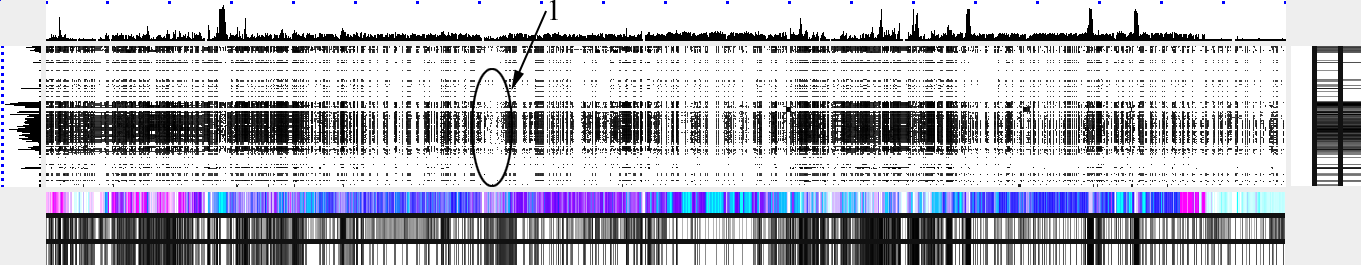
\includegraphics[width=1.0\textwidth]{lviz/boot-dp.png}
\caption{Time-ordered \VDP{} comparing boot
of a clean (Y axis) and a dirty (X axis) system.
}
\label{fig:boot-dp}
%\begin{tabular}{ll}
%DP match : & program + operation + parameter\\
%DP color : & black $\rightarrow$ any\\
%Bar1 color : & cyan $\rightarrow$ Google Desktop; magenta $\rightarrow$ AVG\\
%Bar2 color : & black $\rightarrow$ any program except Google Desktop and AVG\\
%Bar3 color : & black $\rightarrow$ file operation on Windows system directories\\
%\end{tabular}
{\it DP match}: program + operation + parameter;
{\it DP color}: black $\rightarrow$ any;
{\it Bar1 color}: cyan $\rightarrow$ Google Desktop; magenta $\rightarrow$ AVG;
{\it Bar2 color}: black $\rightarrow$ any program except Google Desktop and AVG;
{\it Bar3 color}: black $\rightarrow$ file operation on Windows system directories.
\end{figure*}

In Fig.~\ref{fig:boot-dp}, we use \lviz{} to investigate system boot and try to identify possible
factors causing a system to boot slowly.
To do this, we use a time-ordered \VDP{} to
compare a clean system which is known to boot quickly
with a (dirty) system which has many programs installed and boots slowly.

We see that the clean system boots much faster than the dirty system 
as the height is much shorter than the width.
Whenever Bar2 on the x-axis is not black,
the AVG (AVG antivirus) or Google Desktop is responsible for events.
We see that most of the events in the dirty boot are due to AVG or Google
Desktop.
We can also see from comparing Bar2 with Bar3
that the dirty system has other installed programs running
which are not in Windows directories.
%By looking at Bar1, we can clearly see that Google Desktop and AVG comprise about 5\% of boot time.

Even ignoring other programs outside the Windows directories,
the slowdown is also due to extra work by programs in Windows
directories.
We can see that this because some of the white DP gaps match up with 
black portions in Bar2 (program from Windows directory), e.g. Region 1.
This can be caused by the modification of the Windows system
by third party programs,
e.g. installing new services which are running in svchost.exe, and adding new registry keys or files
which will be scanned by windows programs.
To find out the details, we can focus on Windows built-in programs which
are identified by Bar3.
Vertical gaps in the Windows built-in program region identify the additional work done
by the Windows built-in programs in the dirty system.
By clicking in Region 1, we found out that the gap is caused by
{\tt svchost} (the generic processes for services) since
the new software installed uses {\tt svchost} to run some services.

%\input{lviz/ex-install}
\subsubsection{Web Browser Benchmark}
\label{sec:wbbench}

\begin{figure}[htb]
\begin{center}
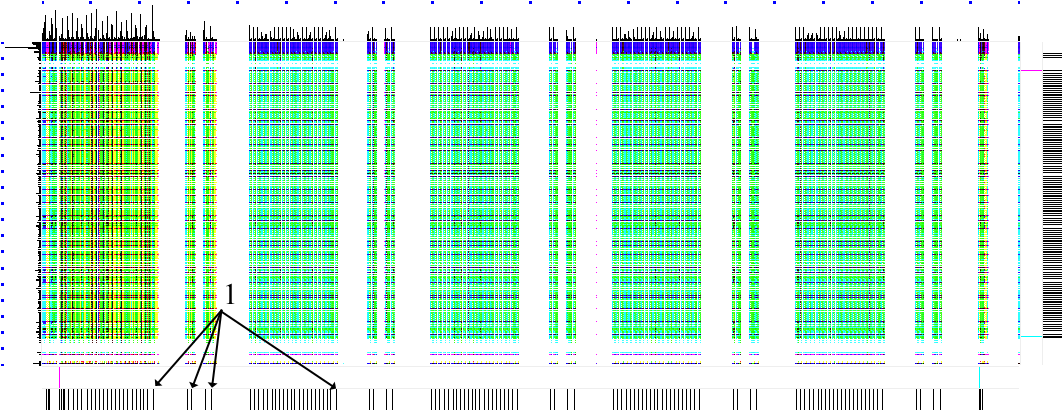
\includegraphics[width=0.7\textwidth]{lviz/wbbench-dp.png}
\end{center}
\caption{Time-ordered VDP comparing IE7 (x-axis) and Chrome (y-axis)
performing the
SunSpider JavaScript benchmark.
}
\label{fig:wbbench-dp}
%\begin{tabular}{ll}
%DP match : & operation\\
%DP color : & cyan $\rightarrow$ file; magenta $\rightarrow$ registry;
%yellow $\rightarrow$ network operation\\
%Bar1 color : & cyan $\rightarrow$ benchmark start time;
%magenta $\rightarrow$ benchmark end time\\
%Bar2 color : & black $\rightarrow$ HTTP GET event
%\end{tabular}
{\it DP match}: operation;
{\it DP color}: cyan $\rightarrow$ file; magenta $\rightarrow$ registry;
yellow $\rightarrow$ network operation;
{\it Bar1 color}: cyan $\rightarrow$ benchmark start time;
magenta $\rightarrow$ benchmark end time;
{\it Bar2 color}: black $\rightarrow$ HTTP GET event.
\end{figure}

We use time-ordered VDP (Figure~\ref{fig:wbbench-dp}) to investigate the
SunSpider JavaScript benchmarks on
two web browsers, Internet Explorer 7 (IE7) and Google Chrome.
The benchmark consists of 26 different tests repeated for 5 times.
Since the browser fetches a web page for each test,
we use the HTTP GET\footnote{
To mark HTTP GET events, we need to turn on network data I/O collection
and use a suitable regular expression as the barcode coloring rule.
The start and end events are marked by matching the two URLs.
}
event (shown in Bar2) to mark the beginning
of each test.
By looking at the time-ordered DP, we know that Chrome is about three
times faster than IE7 in total and also in each test.
From Bar2,
we can also observe that some tests (followed by long white gap,
pointed by marker 1) take much longer time than others.
By clicking on those events, we found out the slow ones to be all string
operation\footnote{
The URLs are \url{/perf/sunspider-0.9/string-base64.html},
\url{/perf/sunspider-0.9/string-tagcloud.html},
and \url{/perf/sunspider-0.9/string-validate-input.html}}
benchmarks.
We conclude that one reason why IE7 is slower than Chrome is due to string operations.

%\input{lviz/ex-iexploit}
%\input{lviz/ex-virus}

\subsection{Conclusion}
\label{sec:lviz-conclusion}

The objective of this work is twofold.
Firstly, we show that visualization can be beneficial for problems
in software understanding and diagnosis. We demonstrate this
for traces with a single program as well as with
several programs and a complete system trace.
Secondly, we show that a DotPlot-based visualization, VDP, is effective
in visualizing a range of problems.
One feature which distinguishes \code{lviz} is that as we work
at the operating system level with system and stack traces,
we do not need source code of the software.
We believe that the range of understanding and diagnosis applications
shows that visualization of operating system traces is an interesting approach.
It also complements other kinds of analysis such
as program analysis and data mining.

Our VDP visualization is only one general purpose visualization.
There are some other problems where dependency visualizations
(Section~\ref{sec:depvis}) or special
variants of VDP would be more appropriate. For example, to understand
resource usage, a special kind of VDP with resources and traces overlaid
with resource lifetimes would give more information than a regular VDP.
We have not taken advantage of source code and this can further enhance
the visualization but it would need monitoring infrastructure which
can correlate execution with the source.
We also remark that although we do not make use of source code, we
see that visualizations using program points can be used to understand
how the code works (at the native code level).

We have developed the VDP tool for Windows because such visualizations
are more beneficial given the closed source nature and system complexity
of Windows.
However, VDP is not reliant on a particular monitoring infrastructure
as the input trace format is very simple.
The same visualization ideas can be applied
to other systems with a rich source of execution traces, e.g. UNIX variants.


\chapter{Binary Integrity} \label{sec:auth}
xxx \cite{wu2009esi}

\clearpage
\section{BinAuth: Secure Binary Authentication}
\label{sec:binauth}

% \subsection{Introduction}
% \label{sec:binauth-intro}

Malware such as viruses, trojan horses, worms, remote attacks, 
are a critical security threat today.
A successful malware attack usually also modifies
the environment (e.g. file system) of the compromised host.
Many of the system security problems such as malware stem from the fact that untrusted code is executed
on the system.
We can mitigate many of these problems by ensuring that code which is executed only comes
from trusted software providers/vendors and the code is executed in the correct context.
In this section, we show that this can be efficiently achieved even on complex
operating systems such
as Windows. Our system provides two guarantees:
(i) we only allow the execution of binaries (in the rest of the section, we refer
to any executable code stored in the file system as a {\em binary})
whose contents are already known and trusted --- we call this {\em authenticating binary integrity};
and (ii) as binaries are kept in files, the pathname of the file must 
match its content --- we call this {\em authenticating binary location}. 
Binary integrity authentication ensures that the binary has not been
tampered with, e.g. {\tt cmd.exe} is not a trojan.
Binary location authentication ensures that we are executing
the correct executable content. 
A following extreme example illustrates location authentication. 
Suppose the binary integrity of the shell and the file system format executables 
are verified. If an attacker swaps their pathnames,
then running a shell would cause the file system to be formatted.
In this section, we refer to {\em binary authentication} to mean when 
both the binary's data integrity and location are verified.

Most operating systems can prevent execution of code
on the stack due to buffer overflow, e.g. NX protection.
Combining stack protection with binary authentication
makes the remaining avenues for attack 
smaller and more difficult.
%i.e. return-to-libc attacks and function pointer overwriting
%are still possible.
Binary authentication is also beneficial because it is even more important
for the operating system to be protected against malicious drivers
and the loading of malware into the kernel.

Most work on binary integrity authentication is on Unix/Linux
\cite{apvrille2004digsig,williams2002anti,doorn01signedexecutables}.
However, the problem of malware is more acute in Windows.
There are also many types of executable code,
e.g. executables (.exe), dynamic linked libraries (.dll), 
ActiveX controls, control panel applets, and drivers. 
In this section, we focus on mandatory binary authentication of all forms
of executables in Windows. 
Binaries which fail authentication cannot be loaded, thus,
cannot be executed. We argue that binary authentication together with 
execute protection of memory regions (e.g. Windows data execution prevention) 
provides protection against most of the malware on Windows.

A binary authentication needs to be flexible to operate under different scenarios.
Our prototype signs binaries using a HMAC \cite{krawczyk1997rfc2104} which is more lightweight
than having to rely on PKI infrastructure, although it can also make use of it.
The authentication scheme additionally allows for other security benefits.
Not only is it important to authenticate software on a system but one also needs
to deal with the maintenance of the software over time.
Nowadays, the number of discovered vulnerabilities grows rapidly 
\cite{CERT-vul}.
This means that binaries on a system (even if they are authenticated) may
be vulnerable. This leads to a vulnerability management and patching problems.
We propose a simple software ID system leveraging on the binary
authentication infrastructure and existing infrastructures such as DNS and certificate authorities
to handle this problem.

Windows has the Authenticode mechanism \cite{authenticode}.
In Windows XP version and earlier, 
it alerts the users of the results of signature verification under
a few situations. However, it is not mandatory, and can be easily bypassed.
The Windows Vista UAC mechanism makes use of signed binaries but it only
deals with EXE binaries. It is also limited to privilege escalation situations.
One common drawback of existing Windows mechanisms is that they do not 
authenticate the binary location.
Moreover, requiring PKI infrastructure and certificates, 
we believe, is too heavy for a general purpose mechanism.
% The latest Windows Vista, through its User Account Control (UAC), 
% makes some improvement by always alerting the users of signature verification status,
% particularly if the user runs with Administrator privilege.
% Yet, many problems remain, such as concern over certificate processing and revocation overhead, 
% and constant interactive user approval dialog which may irritate or annoy the users.

The main contribution of this work is that we believe that it provides the first
comprehensive infrastructure for trusted binaries for Windows.
This is significant given that much of the problems of security on Windows stems from
inability to distinguish between trusted and untrusted software.
It provides mandatory authentication for the full range of binaries under Windows, and goes beyond
authenticated code in XP and Vista.
We also protect driver loading which gives increased kernel protection.
Our scheme provides mandatory driver authentication which 32-bit Windows does not,
and can be integrated with more flexible policies which 64-bit Windows does not support.
We also analyze the security of our system. 
Our benchmarking shows that the overhead of comprehensive binary
authentication can be quite low, around 2\%,
with a caching strategy.
% Caching however is not always better.
% Under intensive file modification usage scenarios, 
% an uncached strategy can be preferable.

% The section is organized as follows.
% Section~\ref{sec:binauth-windows} examines special issues in Windows.
% Section~\ref{sec:binauth-related} surveys related work.
% We describe our scheme and implementation in Section~\ref{sec:binauth-scheme}.
% Section~\ref{sec:binauth-cost} presents the benchmarks, and
% Section~\ref{sec:binauth-conclusion} concludes this section.

\subsection{Windows Issues}
\label{sec:binauth-windows}

We discuss below the complexities and special problems of
Windows which make it more difficult to implement binary authentication
than in other operating systems such as Unix.
Windows NT (Server 2000, XP, Server 2003, Vista) is a microkernel-like
operating system. 
Programs are usually written for the Win32 API but these are
decomposed into microkernel operations. 
However, Windows is closed source --- only the Win32 API is documented
and not the microkernel API.
Our prototype makes use of both the documented and undocumented
kernel infrastructure. However, it is not possible to make any guarantees
on the completeness of the security mechanisms
(which would also be a challenge even if Windows was open source).
Some of the specific issues in Windows which we deal with are:
\begin{itemize}
\item {\bf Proliferation of Binary Types:}
It is not sufficient to ensure the integrity of {\tt EXE} files.
In Windows, binaries can have any file name extension, or even no extension.
Some of the most common extensions include {\tt EXE} (regular
executables), {\tt DLL} (dynamic linked libraries), {\tt OCX} 
(ActiveX controls), {\tt SYS} (drivers), {\tt DRV} (drivers)
and {\tt CPL} (control panel applets).
Unlike Unix, binaries cannot be distinguised by an execution flag.
Thus, without reading its contents,
it is not possible to distinguish a binary from any other file.

\item {\bf Complex Process Execution:}
A process is created using {\tt CreateProcess()} which is a Win32 library
function. However, this is not a system call since Windows is a microkernel,
and in reality this is broken up at the native API into:
{\tt NTCreateFile()}, {\tt NTCreateSection()}, {\tt NTMapViewOfSection()},
{\tt NTCreateProcess()}, {\tt NTCreateThread()}.
Notice that {\tt NTCreatePro-\\cess()} at the microkernel level 
performs only a small part of what is needed to run a process.
Due to this, it is more complex to incorporate mandatory authentication in Windows.

\item {\bf DLL loading:}
To load a DLL, a process usually uses the Win32 API, {\tt LoadLib-\\rary()}.
However, this is broken up in a similar way to process execution above.
% In order to load a particular DLL, a process first calls
% {\tt NtCreate-\\File()} \footnote{A process usually 
% just calls {\tt LoadLibrary()} Win32 API, but we refer to the Native APIs here.}
% to open that DLL file.
% It subsequently calls {\tt NtCreateSection()} to create a section object,
% and then pass the section object to {\tt NtMapViewOf-\\Section()} to map the file 
% into its address space.

%However, many system DLLs known as ``KnownDLLs" \cite{knowndlls},
%on which most executables usually depend on, are loaded differently.
%A registry key defines this set of DLLs.
%They are loaded during system startup by {\tt smss.exe}, and the corresponding section 
%objects are registered in the system so that they can be opened later by 
%calling {\tt NtOpenSection()}.
%This mechanism, although useful for performance reasons, 
%is known to have introduced a security problem in the past \cite{knowndlls-vul}.
% describes a vulnerability in which a user can inject
%a malicious DLL by polluting KnownDlls namespace without modifying any system DLLs.

\item {\bf Execute Permissions:}
Many code signing systems, particularly those on Linux \cite{apvrille2004digsig,doorn01signedexecutables},
implement binary loading by examining the execute permission bit 
in the access mode of file open system-call.
The same mechanism, however, does not work in Windows.
Windows programs often set their file modes in a more permissive manner.
Simply denying a file opening with execute mode set 
when its authentication fails, will cause 
many programs to fail which are otherwise correct on Windows.
Instead, we need to properly intercept the right API(s) with
correctly intended operation semantics to respect Windows behavior.
%We have observed that there are files opened with execute
%permission by Windows Explorer and many other programs but the files are never
%executed.
%In other words, these files are opened with unnecessary execute permissions.
%If these file-open actions are denied, then these programs will not function correctly.

%\item {\bf TOCTTOU:}
%An access control system may suffer from Time-of-Check-to-Time-of-Use
%(TOCTTOU) race condition bug problem \cite{tocttou}.
%In windows, a binary is write-locked during its execution.
%That means, in order to ensure executing the correct file,
%the file only needs to be authenticated at the beginning
%of the execution.
%When the file is from a network file server, the lock is also implemented in the
%file server.
%Thus it has the same semantics as executing a local file.

\end{itemize}

%\TODO{fix version stuff, add brief discussion that windows patches do
%not discuss what files and versions are changed etc}

%Compared to other open platforms, Windows potentially also makes 
%the issue of locating vulnerable software components more complicated. 
%A great deal of binaries created by Microsoft contain an internal file version,
%which is stored as the file's meta-data. After Windows Update operations,
%the name of the updated file may however remain unchanged.
%Thus, it is difficult to keep track of files changes with such embedded version information.
%More precisely, one cannot ensure whether a version of a program $P_i$ 
%remain vulnerable to an attack $A$.
%Without an explicit mechanism like our software naming,
%manual inspection of files therefore is a difficult and daunting task.
%The picture is even made more complicated given that much of 
%Windows infrastructure remains undocumented. 
%As such, it is extremely difficult for a typical administrator
%who examines vulnerability information from public advisories
%to trace through the system and pinpoint the exact affected components.

Compared to other open platforms, Windows potentially also makes 
the issue of locating vulnerable software components more complicated. 
A great deal of binaries created by Microsoft contain an internal file version,
which is stored as the file's meta-data. The Windows update process does not
indicate to the user which files are modified. 
Moreover, meta data of the modified file might still be kept the same.
Thus, it is difficult to keep track of files changes in Windows.
More precisely, one cannot ensure whether a version of a program $P_i$ 
remain vulnerable to an attack $A$.
It is rather difficult for a typical administrator
who examines vulnerability information from public advisories
to trace through the system and pinpoint the exact affected components.
Our software naming scheme, associates binaries with
their version and simplifies software vulnerability management.

\section{Related Work}
\label{sect:related}

Tripwire \cite{KS93} is one of the first to do file integrity protection
but is limited as it in user-mode program and 
checks file integrity off-line.
It does not provide any mandatory form of integrity checking and
there are many known attacks such as:
file modification in between authentication times,
and attacks on system daemons (e.g. cron and sendmail)
and system files that it depends on \cite{Arnold,SKO05}.

There a number of kernel level binary level authentication implementations.
These are mainly for Unix
such as DigSig \cite{digsig}, Trojanproof \cite{williams}
and SignedExec \cite{signedexec}, which modify the Unix kernel
to verify the executable's digital signature before program execution.
DigSig and SignedExec embed signatures within the the elf binaries.
For efficiency, DigSig employs a caching mechanism to avoid checking
binaries which have been verified already. The mechanism is similar 
to ours here but we need to handle the problems of Windows.
It appears that DigSig provides binary integrity authentication
but not binary location authentication.\footnote{Mechanisms based solely on
signatures embedded in the binaries do not have sufficient information
for binary location authentication.}
In this paper, we examine the implementation issues and tradeoffs
for Windows which is more complex and difficult than in Unix.

Authenticode \cite{authenticode} is Microsoft infrastructure
for digitally signing binaries.
% It was publicly announced in 1996 as part of Microsoft's IE 3.0
% and ActiveX technologies, but it ships as a standard part of Windows.
% It tells where binaries come from and checks the integrity of binaries.
In Windows versions prior to Vista, such XP with SP2,
it is used as follows:
\begin{enumerate}
\item During ActiveX installation:
Internet Explorer uses Authenticode to examine the ActiveX plugin 
and shows a prompt which contains the publisher's information
including the result of the signature check.
\item A user downloads a file using Internet Explorer:
If this file is executed using the Windows Explorer shell,
a prompt is displayed giving the signed the publisher's information.
Internet Explorer uses an NTFS feature called
Alternate Data Streams to embed the Internet zone information --in this case,
the Internet-- into the file.
The Windows Explorer shell detects the zone information and displays the prompt.
This mechanism is not mandatory and relies on the use of zone-aware programs,
the browser and GUI shell cooperating with each other.
Thus, it can be bypassed.
\end{enumerate}

Since Authenticode runs in user space,
it can be bypassed in a number of ways, e.g. from the command shell.
It is also limited to files downloaded using Internet Explorer.
Only the EXE binary is examined by Authenticode, but DLLs are ignored.
One possible attack is then to put malware into a DLL and then
execute it, e.g. with {\tt rundll32.exe}.
Furthermore, Authenticode relies heavily on digital certificates.
Checking Certificate Revocation Lists (CRL) may add extra delay 
including timeouts due to the need to contact CA.
In some cases, this causes significant slowdown.

The latest Windows Vista improves on signed checking
because User Account Control (UAC) can be configured for
mandatory checking of signed executables.
However, this is quite limited since the UAC mechanism only
kicks in when a process requests privileged elevation,
and for certain operations on protected resources.
UAC is not user friendly since there is a need for constant
interactive user approval.
% of elevation requests and operations.
% maybe no space to have \cite{vista-complaints}.
Vista does not seem to prevent the loading of unsigned DLLs and 
other non EXE binaries. 
The 32-bit versions of Windows (including Vista) do not checked whether
drivers are signed.
However, the 64 bit versions (XP, Server 2003 and Vista) require
all drivers to be signed (this may be too strict and restrict hardware choices).

The closest work on binary authentication in Windows is
the Emu system in by Schmid et al. \cite{EMU}.
They intercept process creation by intercepting the NtCreateProcess system
call. It is unclear whether they are able authenticate all binary code
since trapping at NtCreateProcess is not sufficient to deal with DLLs.
No performance benchmarks are given, so it is unclear how 
if their system is efficient.

% Since it is important to find out whether the performance penalty due to the 
% authentication is acceptable, this question thus remains unanswered there.
% In addition, our paper here addresses a much wider scope of 
% secure program distribution and execution, taking into account various involved 
% parties (OS, software developers, advisory centers).
%The proposed scheme calculates MD5 hash values of the binaries,
%which are used together with the binary name to uniquely identify an application.
%Each user on the system has an {\em execution control list} (ECL)
%that specifies which applications the user is allowed to execute.
%Although we share the same basic mechanism of in-kernel authentication checking with \cite{EMU},
%our paper here addresses a much wider scope of secure program distribution and execution.
%Firstly, we first ensure that the binary must come with a valid digital signature first
%before generating the MAC for faster integrity checking.
%Secondly, we aim to also find out how low the performance penalty due to the integrity
%checking in Windows environments can be, and whether such penalty is acceptable.
%As no benchmark results shown in \cite{EMU}, the question thus remains to be answered.
%Thirdly, due to our bigger scope, our scheme deals with other new techniques
%such as software naming for vulnerability checking,
%and addresses how various parties (OS, software developers, advisory centers)
%can take advantage of the benefits brought.

% Another approach is to check simply at the filesystem layer such as
% \cite{i3fs}.
% Files are digitally signed,
% and the signature is checked every time the file is accessed.
% This has the drawback that the overhead of authentication is applied
% to all files accessed. For example, in Windows checking for file open with
% execute permissions will lead to many unnecessary checks.
% \TODO{check if the reference summary is correct for i3fs and FS approach}

% On discovering any failure in integrity check,
% the file-system layer will immediately block access to the files and notify the administrator.
% Although such approach can be useful, we view that it is not really suitable
% for our setting in ensuring a wider scope of secure software distribution and execution,
% in which many external parties are involved together.
% 
% [plus the work from LNCS]

\subsection{BinAuth and Software IDs}
\label{sec:binauth-scheme}

We now present our binary authentication system, BinAuth.
We want a lightweight binary authentication scheme which can work
under many settings without too much reliance on other infrastructure.
Furthermore, it should help in the management of binaries, and incurs low overhead.
Management of binaries includes determining which binaries should be
authentic, dealing with issues arising from disclosed vulnerabilities,
and software patching.

\subsubsection{Software ID Scheme}

% \TODO{Cover the case if binary is not signed by developer.
% Remember we want to be lightweight so there are a few possibilities.
% The MAC can be computed at install/first use or it could be signed with
% a digital signature by the user/system administrator with a well known
% public key.}

We complement binary authentication with a software ID scheme meant
to simplify binary management issues.
The idea is that a {\em software ID} associates a
unique string to a particular binary of a software product.
The software ID should come either from the software developer
or alternatively be assigned by the system administrator.
The key to ensuring unique software\_ID, even among different
software developers, lies on the standardized format of the ID.
We can define software\_ID as follows:
\begin{center}
\small
Software\_ID ::= $\langle$ opcode\_tag $\mid\mid$ vendor\_ID $\mid\mid$ 
product\_ID $\mid\mid$ module\_ID $\mid\mid$ version\_ID$\rangle$.
\footnote{Module\_ID suffices to deal with software versioning.
Having a separate version\_ID, however, is useful to easily
track different versions (or patched versions) of the same program.}
\end{center}
\noindent 
Here, $\mid\mid$ denotes string concatenation.
Opcode\_tag distinguishes different naming convention, eg.
$Software\_ID$ and $Custom\_ID$ defined below.

Ideally, we want to be able to uniquely assigning vendor\_IDs to
producers of software which can make the software\_ID unique.
This problem in practice might not be as difficult as it sounds since
it is similar to domain name registration or the assignment
of Medium Access Control (MAC) addresses by network card manufacturers.
One can leverage on existing trust infrastructures to do this.
For example, the responsibility for unique and well known software\_IDs
can be assigned to a Certificate Authority (CA), which then 
define the vendor\_ID as $\langle$ CA\_ID $\mid\mid$ vendor\_name $\rangle$. 
Alternatively, one might be able to use the domain name of the 
software developer as a proxy for the vendor\_ID.

% as
% As we see an increasingly common trend of software developers having
% a certificate, it is thus possible that the assignment responsibility be
% collocated to Certificate Authority (CA). The CA can establish 
% trust management of this software issuer, possibly by including
% added information in the certificate.
% Thus, vendor\_ID ::= $\langle$ CA\_ID $\mid\mid$ vendor\_name $\rangle$
% is sufficient to guarantee unique vendor string information.
%Another example would be the domain name registration where the responsibility
%is also co-located in a organized hierarchical way.

A software\_ID gives a one to one mapping between the binary and its ID string.
This is useful for dealing with vulnerability management problems \cite{sufatrio2004amo}.
Suppose a new vulnerability is known for a particular version of a software.
This means that certain binaries, providing that they correspond to that
software version may be vulnerable. However, there is no simple and standard
way of automatically determining this version information.
Once we have software\_IDs associated with binaries then one can check
the software\_ID against vulnerability alerts. The advisory may
already contain the software\_ID. 
Automatic scanners can then be used
to tie-in this checking with the dissemination of vulnerability alerts
to automatically monitor/manage/patch the software in an operating system.
General management of patches in an operating system can also be done
in much the same way.

In the case where no software\_ID comes with a software product,
one can alternatively derive one.
It can be constructed, for instance, using the following (coarse-grained) string naming:
\begin{center}
\small
$Custom\_ID$ ::= $\langle$ opcode\_tag $\mid\mid$
$hash$(vendor\_URL + product\_name + file\_name + salt) $\rangle$.
\end{center}
The salt expands the name space to reduce the risk of a hash function collision.
% This strategy should provide us with a reasonably reliably mechanism 
% to assign a unique string provided that no collision due to the hash function occurs.

\begin{figure}[tb]
\begin{center}
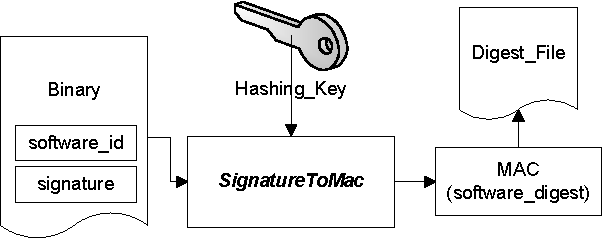
\includegraphics[width=0.6\textwidth]{binauth/hashing}
\caption{SignatureToMac: Deriving the MAC}
\label{fig:hashing}
\end{center}
\end{figure}

\subsubsection{BinAuth System Architecture}

% \TODO{Password issues:
% Password not stored on the machine.
% During the early part of boot, the password could be entered into
% the system or obtained through any secure means which is outside the control
% of the machine.
% What about user passwords?? Still going to have it or not??
% Its feasible but one still has to deal with the boot phase.}

% The key to our lightweight authentication is the derivation
% of a MAC from a binary's valid digital signature.

In the following discussion, we assume here that binaries already come 
tagged with a software\_ID. 
During the BinAuth set-up, preferably done immediately after 
the targeted binary installation, we generate the MAC values for each binary.
In the case where binaries are digitally signed by its developer,
then we verify the signature and then generate the MAC for each binary.
Thus, only one public-key operation needs to be done at install time.
We choose to use a keyed hash, the HMAC algorithm \cite{krawczyk1997rfc2104},
so there is a secret key for the administrator. This is mainly to increase
the security of the stored hashes.
To authenticate binary integrity for any future execution of the code,
only the generated HMAC needs to be checked.
% NO space
% \footnote{
% There are subtle trust issues 
% in the event of certificate expiration/revocation, 
% see Sec. ~\ref{sec:binauth-analysis}.}
In what follows, we mostly write MAC which already covers the choice of HMAC.

One way of storing the generated MAC is by embedding it into the binary.
However, doing so may interfere with file format of the signed binaries
and may also have other complications. 
We instead use an authentication repository file
which stores all the MAC values of authenticated binaries
with their pathnames.
During the boot-up process, the kernel creates its own in-memory data structures
for binary authentication from this file. 
We ensure that the repository file is protected from further modification
except under the control of the authentication system to 
add/remove binaries.\footnote{
Further security can be achieved by integrating binary authentication
with a TPM infrastructure. We do not do so in the prototype as that is
somewhat orthogonal.
}
We can also customize BinAuth on a per user basis rather
than system-wide which is a white-list of
binaries approved for execution.
% Having a MAC repository like this additionally allows us to
% perform the authentication per user basis rather than system-wide.
% Each user in the system thus can have his/her own list of approved binaries.
% This infrastructure thus can readily implement user's application control list
% as in \cite{EMU}.
In the case, when the initial binary does not have a digital signature, then
the administrator can still choose to approve the binary and generate a MAC
for it.

There are two main components of the system: the {\bf SignatureToMac} and {\bf Verifier}.
The SignatureToMac maintains the authentication repository, {\it Digest\_file}, 
consisting of $\langle$path, MAC$\rangle$ tuples.
The Verifier is a kernel driver which makes use of
{\it Digest\_file} and
decides whether an execution is to be allowed.

%\subsubsubsection{SignatureToMac}
\paragraph{SignatureToMac}

Once software is installed on the system,
Fig. \ref{fig:hashing} shows how SignatureToMac processes the binaries:
\begin{enumerate}
\item Checks the validity of the binary's digital signature.
If the signature is invalid, then report failure.
%This step is one where public-key and PKI operation are ever done for each binary.
\item It consults the user or system administrator whether 
the software is to be trusted or not (this is similar to the Vista UAC 
dialog but only happens once).
Other policies (possibly mandatory) can also be implemented.
\item It generates the MAC of the binary 
(including software\_ID string) using a secret key, {\it Hashing\_key}, 
to produce {\it software\_digest}.
The {\it Hashing\_key} is only accessible
% stored in a protected file which can only be accessed 
by the authentication system, e.g. obtained on bootup.
\item It adds an entry for the binary as a tuple $\langle${\it path name}, 
{\it software\_digest}$\rangle$ into the {\it Digest\_file} repository
and informs the Verifier.
The repository is protected against modification. Note that because the entries
are signed, the repository can be read for other uses, e.g.
version control and vulnerability management.
\end{enumerate}

% In order to ensure smoother authentication of all binaries on a system,
% there ideally should be a mechanism that allows system administrator to 
% list all newly added binaries after a software installation.
% Complying installer is thus appreciated to produce such list;
% or alternatively the administrator can deploy a tool 
% which monitors binaries addition during installation.

\begin{figure}[tb]
\begin{center}
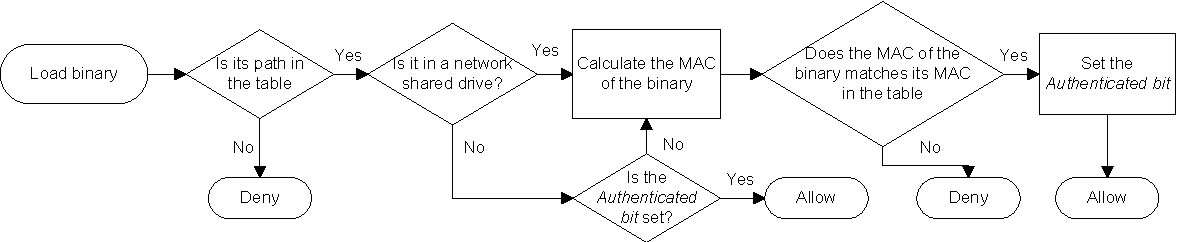
\includegraphics[width=1.0\textwidth]{binauth/verifier}
\caption{Verifier: The Verifier in-kernel authentication process}
\label{fig:verifier}
\end{center}
\end{figure}


%\subsubsubsection{Verifier}
\paragraph{Verifier}

% The Verifier initializes itself from {\it Digest\_file}.
The Verifier performs mandatory binary authentication ---
it denies the execution of any kind of Windows binary which
fails to match the MAC and pathname.
There are two general approaches for the checking.
One is {\em cached MAC} which avoids generating the MAC for
previously authenticated binaries.
The other is {\em uncached MAC} which always checks the MAC.
As we will see, they have various tradeoffs.
The cached MAC implementation needs to ensure that binaries are unmodified.
Hence, the Verifier monitors the usage of previously authenticated files 
on the cache, and removes them from the cache if it can be potentially modified.

The core data structure of the Verifier component can be viewed
as a table of tuples in the form
$\langle${\it Kernel\_path}, {\it FileID}, {\it MAC}, 
{\it Authenticated\_bit}$\rangle$
representing the allowed binaries.
It is indexed on {\it Kernel\_path} and {\it FileID} for fast lookup.
The fields are as follows:
\begin{itemize}
\item The {\bf {\it Kernel\_path}} is Windows kernel (internal) pathname 
representation of a file.
In Window's user space, a file can have multiple absolute pathnames, due to:
(i) 8.3 file naming format, e.g.
``{\tt C:\linebreak[0]$\backslash$\linebreak[0]Program Files\linebreak[0]$\backslash$\linebreak[0]}''
and
``{\tt C:\linebreak[0]$\backslash$\linebreak[0]progra$\sim$1\linebreak[0]$\backslash$\linebreak[0]}''
are the same;
(ii) symbolic links (reparse points is similar);
% to directories/files;
(iii) hard links;
(iv) volume mount points;
% \cite{ntfs-junction} 
or
(v) the {\tt SUBST} and {\tt APPEND} DOS commands.
% \cite{subst}.
The {\it Kernel\_path} is a unique representation for all
the possible pathnames.
% In the kernel, different pathnames referring to the same file 
% are resolved to a unique kernel name, which we use here.
When the system loads $\langle${\it path name}, {\it software\_digest}$\rangle$ 
from {\it Digest\_file} during the startup, {\it path name} is converted to 
{\it Kernel\_path} since all subsequent checks by Verifier in the kernel 
all use the latter.

\item The {\it FileID} is a pair of $\langle${\it device\_name}, {\it NTFS\_object\_ID}$\rangle$.
The {\it device\_name} is a Windows internal name to identify a 
disk or partition volume.
For instance, the device name {\tt HarddiskVolume1} usually refers to {\tt C:$\backslash$}.
The {\it NTFS\_object\_ID} is a 128-bit length number uniquely identifying
a file in the file system volume (this is not the same as Unix inode numbers)
% \cite{objid}.
The Verifier uses the {\it FileID} 
% \cite{hardlink}.
to identify the same file given more than one hard link.
This prevents an attacker from creating a hard link for modifying
a binary without invalidating the binary cache.
The {\it FileID} values will be queried from the system and 
filled into the table during system boot.

\item The {\it MAC} is same as a {\it software\_digest} entry in {\it Digest\_file}.
Our prototype implements the
HMAC-MD5 \cite{krawczyk1997rfc2104}, HMAC-SHA-1 
and HMAC-SHA-256 \cite{eastlake2006rfc4634} hash algorithms.\footnote{
Due to recent concerns which show weaknesses and attacks against MD5 \cite{wang2005break}, 
we also have stronger hash functions, namely SHA-1 and the stronger SHA-256.}
\item The {\it Authenticated\_bit} remembers whether the binary has
been previously authenticated.
It is initially set to false, and set to true after successful authentication.
\end{itemize}

\noindent
Fig. ~\ref{fig:verifier} shows the authentication process 
when a binary executes/loads:
\begin{enumerate}
\item It checks if the binary's {\it Kernel\_pathname} exists in the table.
If not, then deny the execution and optionally log the event.
A notification is accordingly sent to the user. 
% asking to first perform {\it SignatureToMac} step.
\item It the file is on a network shared drive, goto step 4.
The MAC is always
recomputed as we cannot keep track of modification to files on network shares.
\item If the {\it Authenticated\_bit} is set go to step 7.
\item It performs MAC algorithm operation on the binary.
\item If the resulting MAC doesn't match with the 
{\it MAC} stored in the table, execution is denied.
\item It sets the {\it Authenticated\_bit} of the binary.
\item It passes the control to the kernel to continue the execution.
\end{enumerate}

To control binary execution, we intercept the section creation action 
({\tt NtCreateSection()} system call) which is better than:
% As also discussed in \cite{bassov}, intercepting ({\tt NtCreateSection()}
% is a better option than two other alternatives:
\begin{itemize}
\item Intercepting file opening ({\tt NtCreateFile()} and {\tt NtOpenFile()}).
This would need to authenticate any file opened with with execute access mode.
As discussed in Sec.~\ref{sec:binauth-windows}, however, this introduces
unnecessary overheads and can cause some correct programs to fail if the files
do not pass authentication.
There are also technical difficulties to distinguish between
process creation and regular file IO operations, which is not always easy given
its microkernel nature.
%  \cite{bassov}.
\item Intercepting process creation ({\tt NtCreateProcess()}).
This method is not effective for our purpose.
%since it is possible to create a process without calling this system call,
%such as {\tt CreateProcess()}.
Firstly, we cannot use it to control {\tt DLL} loading.
Secondly, it is more difficult to get the pathname of the binary because
process creating is broken down into microkernel operations.
\end{itemize}
It turns out that since all code from any kind of binary
needs to have a memory section to execute,
it suffices to intercept {\tt NTCreateSection()}.

The cached MAC verifier needs to ensure that binaries which have
been already authenticated are not modified.
However, the uncached verifier will not need to perform file monitoring.
%For each entry of the table, we use the {\it Authenticated\_bit} 
%in order to keep track of whether the binary has been previously authenticated.
%Initially, all these bits are set to false.
%The bit is set to true when the binary is authenticated, and set back to
%false when the binary is modified.
A binary with pathname $P$ is considered modified, if the following occurs:
\begin{itemize}
\item $P$ is created: Hence, we monitor system call
{\tt NtCreateFile()} and {\tt NtOpenFile()}.
\item $P$ is opened with write access mode: the previous two
system calls are also intercepted for this purpose.
\footnote{An alternative way is to monitor the file (block) writing operation ({\tt NtWriteFile()}).
However, it is less efficient because file block writings take place more frequently
than file openings as one opened file for modification might be subject to 
multiple block writings. Furthermore, it cannot capture file-memory mapping.}
\item Another file is renamed to $P$: 
We monitor file renaming ({\tt NtSetInformationFile\linebreak[0](\linebreak[0]FileRenameInformation\linebreak[0])})
system call.
\item A drive containing $P$ is mounted:
We monitor drive mounting {\tt IRP\_MJ\_VOLUME\_MOUNT}.
\end{itemize}

\noindent
Note that we do not need to monitor file deletion since we only care about
executing correct files but not missing files.
The details of file modification monitoring are given in Fig. \ref{fileopen}.

Upon modification of $P$, we reset the {\it Authenticated\_bit} of binary $P$, 
and update the {\it FileID} in the table if it is changed.
Should FAT file system be used, pathname is used 
to identify the binary as {\it FileID} is not supported but
neither are hard and soft links.
% Additionally, hard links will not cause any security problems in FAT
% as they are not supported. 
Since {\it FileID} is optional and can be removed,
we monitor {\it FileID} removal ({\tt NtFsControlFile(FSCTL\_DELETE\_OBJECT\_ID)})
and deny the removal if the {\it FileID} is in the table.
Dut to the semantics of NTFS, our use of {\it FileID} can
coexist with other applications using it.

If additional hardware and infrastructure is available to support
secure booting, such as the Trusted Platform Module (TPM) initiative,
the system can benefit from increased security.
Offline attacks would have to first attack the TPM.
The Hashing\_key can also be stored securely by the TPM.

% In an infrastructure where additional hardware is available to ensure secure startup,
% such as recent initiative of Trusted Platform Module (TPM),
% then increased security level can be expected on the authentication system.
% For instance, the Hashing\_key can then be securely stored on the chip
% as opposed to the file system.
% Note that, due to the closed-source nature of Windows,
% it is hard to ensure completeness and soundness with regard to file modification monitoring.
% However, the outlined mechanisms should be sufficient
% to measure the effect of system overheads to provide cache mechanism in
% real-world OS like Windows.

\begin{figure}[tb]
\scriptsize
\begin{center}
\begin{verbatim}
procedure UponModification (FilePath)
   if (FS is NTFS)
      FileID := GetFileID(FilePath) # FileID can be NULL
      if (FilePath is in the table)
         Entry := LookupTableByPath(FilePath)
         if (FileID == NULL)
            # this can happen when the file is deleted and created again.
            # generate a new FileID and update the table
            Entry.FileID := CreateFileID(FilePath)
         else if ( FileID != Entry.FileID in the table)
            # this can happen when the drive is unmounted,
            # id changed off-line and re-mounted
            Entry.FileID := FileID
         end if
         Entry.Authenticated := false
      else if ((FileID != NULL) AND (FileID is in the table))
         Entry := LookupTableByID(FileID)
         Entry.Authenticated := false
      end if
   else if ((FS is FAT) AND (FilePath is in table))
      Entry := LookupTableByPath(FilePath)
      Entry.Authenticated := false
   end if
end procedure
\end{verbatim}
\end{center}
\caption{Pseudo code of file modification monitor}
\label{fileopen}
\end{figure}
\subsubsection{Security Analysis}
\label{sec:binauth-analysis}

The security of BinAuth relies on the strength
of the chosen hash functions (MD5, SHA-1, SHA-256) as well as
the HMAC algorithm.
Thus, we assume that any change in a binary can be detected through a changed MAC.

In our authentication on binary with digital signature, 
the subsequent invocations using MAC verification is sufficient 
to ensure the authenticity of the binary.
In other words, MAC authentications ``{\em preserve}'' the previously
established properties of BinAuth derived from digital signature.
A subtlety comes when the certificate expires or is revoked 
at some point in time after SignatureToMac.
We view that the question of whether one should keep trusting the binary for execution
depends on one's level of trust on certificate expiration/revocation.
If the certificate expiration or revocation means 
that the public key must no longer be used,
but the fact that {\em previously established} goodness binary properties still hold,
then we can keep trusting the binary for execution (as long as we still believe the issuer).

% \item {\it ``Provided that the Hashing\_key is good, any corruption of
% a binary's  software\_digest (MAC) in Digest\_file will result in a failed verification''}:\\
% %Informal Proof:\\
% As the hash on the binary is done with Hashing\_key,
% any corrupted software\_digest will thus result in a mismatch.
% This higher level of protection guarantee is the reason
% why we employ MAC algorithm (using Hashing\_key) instead of keyless hash operation.
% Although we can assume that digest\_file is stored securely,
% having a separate Hashing\_key provides increased protection.
% A highly secure system can then be achieved, for example, by having
% Hashing\_key stored in a more secure (tamper-resistant) storage.
% Given the key's short length, thus only very small memory requirement 
% on the storage is imposed in trade of higher security guarantee.
% \end{itemize}

% \subsubsection{Threat Analysis}
Here we discuss some possible attacks to the authentication system.
All the attacks except the last two target the caching system.
More precisely, the attacker attempts to modify an already authenticated
binary without causing the {\it Authenticated\_bit} to be set to false.

\begin{itemize}
\item {\bf Manipulating symbolic links:}
The attacker can use the path $S$ which is a symbolic link of an authenticated $P$
to indirectly modify $P$ and subsequently execute $P$.
However, the modified file will not be executed successfully, because
Windows kernel resolves symbolic links to real paths.
More precisely, the symbolic link $S$ is resolved to the real path $P$.
As a result, the {\it Authenticated\_bit} of $P$ will be set to false.
When $P$ is executed, its MAC will be recalculated and it will not pass
the authentication.

\item {\bf Manipulating hard links:}
The attacker can create a hard link $H$ on an already authenticated file $P$
and then modifies the file using path $H$.
This attack will not succeed because we use {\it FileID} to identify files.
$H$ has the same {\it FileID} as $P$,
thus the {\it Authenticated\_bit} will be set to false.
Note that this attack will not succeed in FAT file system either,
even though we cannot use {\it FileID}.
This is because hard link is not supported in FAT.

\item {\bf Manipulating FileID:}
Recall that {\it FileID} consists of {\it device\linebreak[0]\_\linebreak[0]name}
and {\it NTFS\linebreak[0]\_\linebreak[0]object\linebreak[0]\_\linebreak[0]ID}.
The latter is optional and thus can be removed.
The attacker can remove the {\it NTFS\_object\_ID}, and then performs the previous attack.
We handle this attack by denying {\it NTFS\_object\_ID} removal on authenticated files.
This is implemented by monitoring the file system control event {\tt FSCTL\_DELETE\_OBJECT\_ID}

\item {\bf Remote File Systems:}
Since we cannot keep track of modification on a network shared file system,
we do not cache the authentication.
More precisely, the MAC of the binary is always calculated upon loading.
Same applies to removable media such as floppy in which we can not
keep track of modification of files.

\item {\bf TOCTTOU:}
TOCTTOU stands for Time-Of-Check-To-Time-Of-Use.
It refers to a race condition bug of an access control system
where the resource is changed during the time
of checking the resource to the time of using the resource.
In the BinAuth context, the binary may be modified
after the time it is authenticated and before the time it is executed.
However, we observed that all binaries are exclusive-write-locked
when it is opened.
That means binaries cannot be modified from the time it is opened
to the time it is closed.
Also note that the file is authenticated after it is opened and before
it is executed.
As a result, binaries cannot be modified during TOCTTOU.

When the binary is in a network shared volume, i.e. SMB share,
and the write-lock is not properly implemented in the SMB server,
an attacker is able to modify the binary after authentication.
However, we have observed that both Windows and Samba
implement write-lock properly.
Thus the attack is only possible when the SMB server is compromised.
One way to prevent this is to disallow binary loading from SMB share.

\item {\bf Driver Loading:}
BinAuth authenticates all binaries including kernel drivers.
This means all drivers are authenticated thus driver attacks such as
kernel rootkits and malware drivers can be prevented.

\item {\bf Offline Attack:}
Offline attack means modification of the file system when Windows is
not in control.
For example, boot another OS or remove the disk drive for
modification elsewhere. Such an attack will require physical access
to the machine. Offline attack can corrupt data or change programs/files
and affect the general functioning and we cannot prevent that.
What we can do is to ensure the integrity of executable code and other data
loaded in memory for processes.

We assume that the kernel is still secure, i.e. authentication occurs early
in the boot.
% and the kernel itself has been authenticated by the boot loader.
We also assume that kernel functioning is not impaired, e.g. deleting some
system files does not cause the kernel to have an exploitable vulnerability.

Since the hashing\_key is not stored in the machine, it is not available
to the attacker.
The attacker can still change the digest file and the binaries,
however, MACs of modified binaries cannot be produced without the hashing\_key.
Thus modified binaries cannot be executed when the system is online.
\end{itemize}

\subsection{Empirical Results}
\label{sec:binauth-cost}

Our authentication system can detect when a modified binary is loaded
or run from the wrong pathname. In this section, we examine
the three factors which impact on system performance:
(i) Verifier checking upon binary loading (execution);
(ii) file modification monitoring; and
(iii) binary set-up during the SignatureToMac process.
The first two above are the most important as they directly 
affect user's waiting time for process execution and 
affect overall system operation.
The tests here are meant to determine the worst case overhead as well
as average overheads.

The benchmarks are run on a Core 2 Duo with 2GB of ram
running Windows XP with SP2.
Each benchmark is run five times.
As we want to investigate the effect of the cached Verifier,
each benchmark is run with caching and without caching.
% When caching is disabled, the binaries will be authenticated 
% every time they are executed, and {\tt NtCreateFile()} and {\tt NtOpenFile()} 
% system calls are not intercepted.
When caching is enabled, we ignore the result of the first run because
the overhead of authentication overhead is already shown in the uncached case.
Even if we count the first run, its impact will be very small because
some of the microbenchmarks run for 10K times, so the authentication
overhead becomes negligible.

To see the difference of using different hashing algorithms, we implement
and benchmark three algorithms: MD5, SHA-1 and SHA-256.
Only MD5 and SHA-256 are shown in Table~\ref{table:bigtable} as
the results of SHA-1 are always between these.
When caching is enabled, results of different hashing algorithms are
not distinguished (shown as Cached-MAC in the table),
because binaries are not require MAC checking during the benchmark.
The reason is that the first run is ignored, and the binaries are not modified
during the benchmark.

To see the difference with digital signature based authentication system,
we also compare the performances of our scheme against
the Microsoft official Authenticode utility called {\tt Sign Tool} \cite{signtool},
and another Sysinternals (now acquired by Microsoft) Authenticode utility
{\tt Sigcheck} \cite{sigcheck}.
Note that two tools are user-mode programs.
They are there to illustrate the difference between non-mandatory strategies
used with Authenticode with our in-kernel mandatory authentication.
% However, the slowdown factor can already be seen clearly from the results shown later.

% \subsection{Overhead of Loaded-Binary Verification}

The first two benchmarks investigate system performance under
two scenarios:
\begin{enumerate}
\item {\bf Micro-benchmark:}
The micro-benchmark aims to measure the worst case performance overhead
incurred by the scheme. 
Note that this is primarily intended to measure the authentication cost
but not other overhead, which is done by the last file modification 
microbenchmark.
Here, we have two micro-benchmark scenarios.
\begin{enumerate}
\item {\bf EXE Loading:}
This executes the {\tt noop.exe} program, a dummy program
that immediately exits, for 10K times.
This scenario measures the overhead for authenticating the
{\tt EXE} file.
The benchmark program first calls {\tt CreateProcess()},
and waits for the child process' termination using the {\tt WaitForSingleObject()} function.
We use different binary sizes (40KB, 400KB, 4MB and 40MB, only the 40K and 40MB
results are displayed)
for noop.exe to see how executable size impacts performance.
\item {\bf Loading DLL:}
The second scenario executes the {\tt load-dll.exe} program for 100 times.
This scenario is used to find out how the number of loaded DLLs impacts the performance.
Program {\tt load-dll.exe} loads 278 standard Microsoft
DLLs with a total file size of $\sim$75MB.
The size of the {\tt load-dll.exe} itself is 60KB.
Note that in Windows, the bulk of code is often in DLLs which is why the 
{\tt EXE} file may be small, e.g. Open Office has over 300 DLLs.
\end{enumerate}

\item {\bf Macro-benchmark:}
The macro-benchmark measures overhead under a typical usage scenario.
Our benchmark is to create the Windows DDK sample projects
using the {\tt build} command.
In each test run, 482 C/C++ source files in 43 projects are built.
This benchmark is chosen as it is deterministic, non-interactive, creates
many processes and uses many files.
\end{enumerate}

We benchmark {\tt Sign Tool} and {\tt Sigcheck} in the following fashion.
We first sign {\tt noop.exe} and {\tt load-dll.exe} using 
{\tt Sign Tool}'s signing operation.
We then measure the execution time of 
authenticating and executing the two programs.
For the macro-benchmark, we replace each development tool in the DDK
(i.e. {\it build.exe}, {\it nmake.exe}, {\it cl.exe} and {\it link.exe})
with a wrapper program which first authenticates the actual development 
tool and then invokes it.
For the micro-benchmark, we consider two settings: 
(i) {\tt EXE} only; and (ii) all binaries ({\tt EXE} + {\tt DLL}).
The macro-benchmark, however, only tests the EXE case.
This is because, during the macro-benchmark, many programs are invoked,
and each program each invocation may dynamically load a different set of DLLs.
Thus, it is hard to keep track of what DLLs are loaded, and it is
unfair to simulate with all DLLs used.

\begin{sidewaystable*}
%\begin{table*}[tb]
\centering
\begin{tabular}{|l||c|c||c|c||c|c||c|c|}
\hline
   & \multicolumn{6}{|c||}{{\bf Micro-Benchmark}} & \multicolumn{2}{|c|}{{\bf Macro-}} \\
   & \multicolumn{6}{|c||}{} & \multicolumn{2}{|c|}{{{\bf Benchmark}}} \\
{\bf Authentication}	& \multicolumn{2}{|c||}{{\tt noop} 40K} & \multicolumn{2}{|c||}{{\tt noop} 40M}
   & \multicolumn{2}{|c||}{{\tt load-dll}} & \multicolumn{2}{|c|}{{\tt build}} \\
{\bf System}    & time & slowdown & time & slowdown
                & time & slowdown & time & slowdown \\
\hline
\hline
{\bf Clean}     & $22.76$ & $-$ & $30.07$ & $-$
                & $45.32$ & $-$ & $66.26$ & $-$ \\
\hline
{\bf EXE Only:} & & & & & & & & \\
{\tt Signtool}  & $2822$ & \underline{$11637\%$} & $4850$ & $16033\%$
                & $73.49$ & \underline{$62.16\%$} & $97.00$ & $46.39\%$ \\
{\tt Sigcheck}  & $1720$ & $7457\%$ & $5629$ & $18623\%$
                & $62.82$ & $38.62\%$ & $110.5$ & \underline{$66.72\%$} \\
Uncached-MD5    & $25.96$ & $14.08\%$ & $2150$ & $7052\%$
                & $45.34$ & $0.05\%$ & $70.85$ & $6.93\%$ \\
Uncached-SHA256 & $30.29$ & $33.07\%$ & $9005$ & \underline{$29851\%$}
                & $45.34$ & $0.05\%$ & $71.79$ & $8.35\%$ \\
Cached-MAC      & $23.20$ & ${\bf 1.93}\%$ & $30.63$ & ${\bf 1.88}\%$
                & $45.33$ & ${\bf 0.02}\%$ & $67.62$ & ${\bf 2.06}\%$ \\
\hline
{\bf All Binaries:} & & & & & & & & \\
{\tt Signtool}  & $11867$ & \underline{$52043\%$} & $14030$ & \underline{$46565\%$}
                & $16018$ & \underline{$35244\%$} & $-$ & $-$ \\
{\tt Sigcheck}  & $4283$ & $18772\%$ & $6186$ & $20478\%$
                & $12548$ & $27587\%$ & $-$ & $-$ \\
Uncached-MD5    & $26.10$ & $14.67\%$ & $3881$ & $12811\%$
                & $128.8$ & $184.1\%$ & $79.31$ & $19.69\%$ \\
Uncached-SHA256 & $30.42$ & $33.67\%$ & $9302$ & $30839\%$
                & $201.3$ & $344.0\%$ & $91.80$ & \underline{$38.55\%$} \\
Cached-MAC      & $23.25$ & ${\bf 2.14\%}$ & $30.58$ & ${\bf 1.72\%}$
                & $45.35$ & ${\bf 0.07\%}$ & $67.88$ & ${\bf 2.45\%}$ \\
\hline
\end{tabular}
\caption{Benchmark results showing times (in seconds) and slowdown factors. The worst slowdown
factors for each benchmark scenario are shown with underline, whereas the best are in bold.
We define $slowdown_x = (time_x - time_{clean}) / time_{clean}$.}
\label{table:bigtable}
%\end{table*}
\end{sidewaystable*}

The results are given in Table \ref{table:bigtable} but
we have not shown ``noop 400K'' and ``noop 4M'' 
because they are bounded by the results of ``noop 40K'' and ``noop 40M''.
Other results not shown are that the overhead is approximately
linear with respect to the file size, e.g.
the results of the All-binaries/Uncached/SHA-256 benchmarks are
40K:30.42s, 400K:85.43s, 4M:598.0s, 40M:9302s.

We can see that the overhead of {\tt Signtool} and {\tt Sigcheck} makes
it unusable if DLLs are to be checked (352x slower on {\tt load-dll}).
If only {\tt EXE} are checked, then at least 40\% overhead and based
on the {\tt load-dll} benchmark, one could expect about an order
of magnitude worse if all DLLS are checked.
Of course, using these tools would incur additional overhead from creating
a process and the main purpose is just to show the difference
between what can be done in user-mode versus in-kernel.
We can see that all the uncached-MD5/SHA256 are considerably faster
than {\tt Signtool} and {\tt Sigcheck}.

Authenticating only {\tt EXE}, the difference between uncached has overheads
around 8\% while cached brings this down to very small, around 2\%x and almost
neglible in the {\tt load-dll} benchmark (0.02\%).
Note that as uncached overhead is quite small, the results are dominated
by non-determinism in timing measurements.
Moving to all DLLs ({\tt EXE} + {\tt DLL}), we can see the effect of Windows
programs using many DLLs (more code in {\tt DLL} than {\tt EXE}).
The overhead incurred by caching is still small while uncached can grow 
to between 20-40\% depending on the hash algorithm.
Note that the uncached overhead is applicable for files which cannot be cached.

% \subsection{Overhead of File Modification Monitoring}

%\begin{table*}[h]
%\centering
%\begin{tabular}{|l|c|c|}
%\hline
%Case & time & slowdown \\
%\hline
%Clean & $4.051$ & $-$ \\
%File in the table & $6.809$ & $68.1\%$ \\
%File not in the table & $6.266$ & $54.7\%$ \\
%\hline
%\end{tabular}
%\caption{Benchmark results showing file modification monitoring overhead}
%\label{table:filewrite}
%\end{table*}

The final microbenchmark investigates the tradeoffs between cached
and uncached verification.
Caching means that MAC verification is amortized over executions
but has added overhead from monitoring file modification,
while uncached is the opposite.
% has the cost of MAC every execution 
% but no file modification cost.
Our micro-benchmark opens a file for writing 100K times to
measure the worst case overhead incurred by file modification monitoring.
We have 3 experiments:
(i) a clean system without BinAuth;
%  ($CleanMod$);
(ii) BinAuth with cache and the modified file is a binary;
% ($BinMod$);
and (iii) BinAuth with cache and the modified file
is not a binary.
%  ($DataMod$).

The results for the file modification micro-benchmark
show that for BinAuth with a cache, it
doesn't matter whether the file being written to is a binary or not.
Both cases incur about 60\% overhead compared to a clean system.
Since BinAuth with no-cache has no overheads for file
modifications, this means that under some usage scenarios where file modification
is very high,
the uncached strategy may be preferable over cached even when Verifier overhead
is higher.

% The results show that the running time of $B$ and $C$ are both about 1.6 times of $A$.
% This overhead only happens when a file is opened with write permission.
% There is no overhead when a file is opened with read permissions.
% There is a tradeoff between cached and uncached version.
% When there are a lot of file modifications, the uncached version will be more efficient.

\section{Conclusion}
\label{sect:conclusion}

We have shown a comprehensive system which authenticates both content and pathname
for Windows to ensure that only trusted binaries are executed. 
Unlike other operating systems, Windows poses significant challenges.
We show that it is possible to ensure that only trusted binaries can be loaded
from files for execution. 
This can also be combined with a simple software ID
scheme which simplifies binary version management, and dealing
with vulnerability alerts and patches.
Our system is lightweight and integrates well with PKI and 
trust mechanisms without
having to rely on them.
The overheads of our prototype are quite low when caching is is used.
In the case of workloads with heavy file modifications, an uncached strategy might be preferable.
The overheads are still low in this case, since the system overhead
will be dominated by I/O rather than binary authentication, so the overall binary authentication
would still be low as a percentage of overall system overhead. 
In summary, although this is a prototype, it significantly adds
to the security of any Windows system but at the same time is sufficiently
flexible so that it can be tailored for different usage scenarios.

% In this paper we have performed a study on the feasibility of mandatory
% software component authentication. Our approach uses a lightweight
% authentication technique using MACs. According to our benchmarks, we
% found that using a cache reduces the overhead as it reduces
% the number of repeated authentication requests. 
% Based on these benchmarks,
% we can conclude that our mandatory authentication can be added to Windows
% without significant overhead.
% We have also introduced the concept of ``software naming''. The
% idea behind this is to uniquely identify a file. We have mentioned a few
% applications for this idea.
% Given the security benefits of binary authentication and software naming,
% and only small overhead incurred even on complex OS like Windows,
% we envisage that the presented results can better convince 
% the OS and user community alike to start deploying them more universally 
% in realizing secure software distribution and execution.


\clearpage
\section{Towards a Binary Integrity System for Windows}

% \subsection{Introduction}

The previous section showed BinAuth, a reliable and efficient system
to authenticate binaries in Windows.
It is designed for environments where the binaries are relatively static,
i.e. the binaries rarely change or the changes are well managed by
the system administrator.
However, in systems such as personal machines, it is common for binaries
to change.
In particular, users can install or uninstall software;
The software can perform automatic updates periodically;
and some software creates temporary binaries.

In this section, we first look at the dynamics of binaries and compare
it with attacks in Section~\ref{sec:binint-usageattack}.
We then discuss the related work in Section~~\ref{sec:binint-prevworks}.
After that, we present a new security model for binaries called
{\em BinInt} in Section~\ref{sec:binint-model}.
It provides a number of modes for operation: default, install
and temporary trusted modes.
BinInt provides protection (in default mode) against a broad range of
binary-based attacks.
In Section~\ref{sec:binint-imp}, we show the implementation and
in Section~\ref{sec:binint-secanal}, we analyze the security of
both design and implementation.
In Section~\ref{sec:binint-eval}, we evaluation BinInt in terms of
performance and usability.
Our system is efficient and has negligible overhead in default and temporary
trusted modes. 
In install mode, our benchmarks
show $\sim$12\% overhead which is reasonable since
the use of install mode is infrequent.

\subsection{Windows Binary Security Issues}
\label{sec:problems}

The Windows NT operating system
is difficult to secure
because of its closed source and complex nature.
To understand the issues, we first discuss how
binaries are used in Windows followed
by some representative attacks.

\subsubsection{Binary Usage in Windows}

A {\em binary} in Windows is a file containing executable code.
Binaries in Windows occur in many contexts,
the following is a non-exhaustive list:
applications/executables ({\tt exe}),
command files ({\tt com}),
Dynamic Linked Libraries ({\tt dll}),
ActiveX controls ({\tt ocx}),
device drivers ({\tt drv},
screensavers ({\tt scr}),
control panel applets ({\tt cpl}),
Input Method Editors ({\tt ime}),
and codecs ({\tt acm}, {\tt ax}).
Obviously a binary needs to be in the correct format.
In Windows, the only way to identify a binary
is its format, the filename extension is only a convention.

A single process in Windows typically uses many binaries which
can originate from many sources.
For example, a software installation may introduce many binaries including
shared libraries which can be loaded by many/all processes.
To illustrate, even a small program like {\tt notepad}
loads 13 binaries from 3 different directories.
(It happens here that because the AVG antivirus is installed, the
binary {\tt avgrsstx.dll} is also loaded).
In contrast, {\tt Internet Explorer} on a {\em YouTube} page may load
86 DLLs from {\tt System32}, 14 other DLLs, 3 drivers and some other
binaries.
A more detailed look at the sharing and dependencies of Windows binaries
can be found in \cite{icse10}.

There are numerous mechanisms in Windows which can cause a binary to be used,
i.e. load the binary.
Subsequently, code in the binary may be executed.
Some of the common mechanisms used both by legitimate software
as well as malware are:
DLL injection, DLL search order hijacking, Autorun/Autoplay, Autostart,
shell extensions, Windows Services, {\tt rundll\linebreak[0]32.exe},
and Browser Helper Objects.

\subsubsection{Normal Usage versus Malicious Attacks}
\label{sec:usageattack}

A security model must be able to distinguish
malicious attacks from normal software usage.
We firstly look at typical software usage scenarios in the
software life cycle, namely running, installing, updating and developing 
a software.
We then look at some attacks which exploit binaries whose
behavior is similar to the normal usage scenarios.

The most common scenario is that of {\em running} a software.
Normal usage typically involves loading binaries,
reading/writing data files and possibly the creation of child processes.
It is, however, not common for binaries to be created or modified.
We highlight that binaries can come from
various (3rd party) sources.
For example, Windows Explorer (Windows GUI shell) loads 3rd party DLLs
to provide shell extensions.
The shell extensions are used to preview
images or video, to add a control panel component, to customize
file icons and context menus, etc.
Another example is anti-virus software which forces
its DLLs to be loaded by {\em all} processes, e.g. {\tt avgrsstx.dll}
from the AVG anti-virus software.

{\em Installing} software involves creating binaries
and data files.
Installers downloaded from the Internet are typically packed as
self-extracting archives, which
unpack themselves into a temporary directory and launch from there.
This unpack-and-run behaviour is also observed in the normal
running of some software, e.g.
many {\tt Sysinternals} tools
unpack a kernel driver into a temporary directory and then load it.

There are a number of software {\em update} mechanisms.
Microsoft Windows Update employs a dedicated service (daemon process) to check,
download and apply updates.
In this case, the updater is completely separate from 
the software being updated.
Other software, such as {\tt Mozilla Firefox} and {\tt Sun JDK},
employ a self-update mechanism.
We use Firefox to illustrate the mechanism.
Firefox checks online if there is a new version available and
downloads the update as a compressed archive file.
After downloading, Firefox invokes the updater
as a helper process and terminates itself.
The updater process reads the downloaded archive and 
updates {\tt firefox.exe}
and other files if necessary.
When updating is finished, the updater re-launches Firefox ({\tt firefox.exe})
and terminates itself.
The helper process technique is usually used
because in Windows, a binary cannot be written to when it is loaded by
another process.

Software {\em development} means that binaries have to be created.
For example, to debug a software using an IDE,
the IDE firstly builds the program and then runs it.
Thus the IDE creates or modifies binaries then executes them.

We now turn to some common attacks that involve binary loading or modification.
Furthermore, these attacks use binary vulnerabilities in trusted programs.
We highlight how the attacks behave in a similar fashion to the normal usage
scenarios described earlier and the security mechanism needs
to distinguish between normal usage versus an attack.

\paragraph{Running Unintended Executables}

A common attack is to employ social engineering techniques to get
the user to run a malware executable.
However, the attack can be more subtle and exploit features of various
applications to hide the executable. 
For example, by default, Windows Explorer hides file extensions. 
Consider a malware {\tt postcard.jpg.exe} where
the icon of the malware also looks like a photo.
The user is then fooled into thinking it is a JPEG image and click
it for viewing in Windows Explorer.
The malware could execute its payload and then display
the photo.
Thus, the user would probably think this is just the normal display
of a JPEG image.
Notice that the behaviour of both a direct or file extension social
engineering attack is similar to the regular
software running scenario.

\paragraph{Application Data with Embedded Binaries}

Malware binaries can be embedded within documents.
A recent vulnerability in PDF readers \cite{pdfattack} illustrates this
attack where a legal PDF file containing an embedded executable.
When the PDF file is viewed, the PDF viewer (e.g. {\tt Acrobat}) also
automatically executes the embedded executable.
Notice that the behavior in the attack
resembles the unpack-and-run in the normal installation scenarios.


\paragraph{DLL Attacks}

DLL attacks typically exploit some feature of an application
to inadvertently load a malicious DLL.
The ``carpet bomb'' \cite{safari1} attack involves bugs of two different
browsers.
Safari had a feature\footnote{
Apple did not consider it as a bug.
}
which downloaded files onto the user's desktop automatically.
Internet Explorer had a bug where certain DLLs are specified
by the file name rather than a full pathname.
By combining the behavior of Safari and Internet Explorer,
a malicious website can execute arbitrary code on a machine 
that visits the site.
It is surprising to see that this vulnerability where applications
do not use a sufficiently qualified path when loading DLLs
has recently re-surfaced
(in Aug 2010) as ``binary planting'' attacks \cite{binary-planting}.

In some cases, an application has features to execute binaries.
This can be exploited.
A vulnerability \cite{winhelp} in handling Windows Help files in
Internet Explorer was recently discovered.
A malicious web page can cause Internet Explorer to load a malicious
WinHelp ({\tt .hlp}) file from an arbitrary path.
WinHelp also has a feature to allow loading of arbitrary DLLs.
The bug and the feature together enable a malicious website to execute
arbitrary code on the client.

The recent Stuxnet worm \cite{stuxnet} also uses a DLL attack.
Interestingly, Windows 7 does not even give a UAC warning with this attack.
Stuxnet exploits a vulnerability in Windows Explorer which displays an icon
for shortcut files by using a DLL specified in the shortcut.

All above attacks load existing malicious DLLs which could be accidentally
downloaded/copied or exist in a network drive.
Once the DLL is in place, the behaviour of the attacks is similar to the
regular software running scenario.

\subsection{Related Work}
\label{sec:prevworks}


\subsubsection{Isolation Models}

Isolation can be used to prevent malware from changing
other parts of the system.
A straight forward form of isolation is to have 
multiple independent systems or virtual machines (VM).
This is useful for protecting one application against another though
it might not protect against the PDF and WinHelp attacks discussed in
Sec.~\ref{sec:usageattack} which are against the applications themselves.
There is also the question of whether it is effectively feasible to 
run each software within its own VM.
On the one hand,
this by definition also prevents sharing which is incompatible
with the use of implicit sharing by software in Windows and
may be incompatible with system services and utilities.
It also means a loss of usability since data is not sharable
between applications.
The isolation also leads to high
maintenance cost of updating all VMs against
vulnerabilities as there are multiple copies of
the same software or library.
On the other hand, using isolation separately on each software can also
have significant system overheads since large numbers of virtual machines
need to be run.

One-way isolation is a form of isolation which
lets untrusted programs run in a sandbox where they can read from the
trusted base system but modifications are confined to the sandbox.
In one-way isolation, processes can be executed in isolation domains,
other processes are executed normally in the base system.
The semantics of file access is modified such that an isolated process
can read files in the base system but when it tries to modify them,
a private copy is duplicated from the base system and subsequent modification
is applied on the private copy.
Special care must be taken to handle file deletion so that files in the
base system are not accessed.

Kato et al. proposed an one-way isolation system named
SoftwarePot \cite{kato2003softwarepot},
whose main purpose is to allow software to securely circulate among
different hosts.
Secure circulation means that software in the sandbox should not interfere
with the base system.
A security policy specifies files visible to the sandbox,
path mapping from base system to sandbox, system calls allowed and
network addresses allowed to interact.
Liang et al. proposed another one-way isolation system named
Alcatraz \cite{liang2009alcatraz}.
The main difference between SoftwarePot and Alcatraz is that the latter
enables modification from the sandbox to be {\em committed} to the base
system.

The problems of one-way isolation are similar to that of
virtual machines, namely, that isolation is the opposite of sharing.
Other than that, one-way isolation protects the integrity of non-isolated
system from attackers in the isolated system,
but it does not protect the integrity of the isolated system.
There are many forms of interactions between the sandbox and the base system,
such as file system access, networking and IPC
(including local sockets, pipes, process synchronization mechanisms,
signals, window messages, etc.).
The first two forms are easier to sandbox because their semantics are known.
However, IPC is application dependent and can be complicated and
undocumented.
Even if only considering documented ones,
it would take too much effort to implement filters for different IPC
protocols (e.g. shared memory, pipe, CORBA, D-Bus, SunRPC etc.).
SoftwarePot does not discuss IPC and Alcatraz simply disallows some forms of IPC.
However, IPC is important and cannot be ignored.
For example, the X window system, is implemented as local sockets;
the Windows GUI requires (undocumented) IPC to the {\tt smss.exe}
and {\tt csrss.exe} processes.
Some services are implemented as IPC such as
service management and domain name resolution in Windows,
PulseAudio (the sound system in Linux),
and syslog (the UNIX logging service).
Simply allowing and denying them will lead to either insecure sandboxing or
unusable software.

\subsubsection{Signed Binaries}
\label{sec:signing}

There are systems \cite{halim2008lightweight,apvrille2004digsig,williams2002anti,doorn01signedexecutables,nanda2006fcd}
that only allow signed binaries to be loaded or executed.
In these systems, signature of binaries are either embedded
in the files themselves or signed by a third party, such
as the administrator and stored in a secure database.
Executing or loading are only allowed if the signature can be verified.

There are three basic problems with signed binaries.
Firstly, the security relies on the trust of the signing keys.
If key is leaked, the trust is broken.
For example, the Stuxnet worm \cite{matrosov2010stuxnet} uses
signed drivers with real certificates which are trusted by Windows.
Secondly, revocation checking is expensive as it cannot be done
locally and furthermore may not be timely.
Lastly, we cannot assume that all software vendors sign their binaries.
A more important difference is that most signed binary schemes are not
intended to deal with the software lifecycle issues which we are concerned with.
Another difference is that signed binaries
only ensures that the binaries are not modified but
may not prevent deletion.

\paragraph{Self-signed executables}

Self-signed executables \cite{wurster2007self} is a different approach
to signed binaries which allows for software updates.
In their proposal, all binaries are embedded with their signatures signed
by the software vendor.
Unlike the previous signed binary systems, the assumption is that any
binary which has been signed can be trusted.
Using the observation that binaries are usually updated by a newer
version from the same vendor as the original,
binary updating is allowed if the signature can be verified
with the same public key.

The self-signed executables system binds paths with keys.
Once bound, the key cannot be changed, even when the file is removed.
An attacker can also sign malware as long as it is the first
software installed with that path.
Alternatively, this can constitute a denial of service attack since
an attacker binding the path first would disallow future correct
software to be installed at that path.
As deleted files leave behind a stub, the number of stubs will
monotonically increase over time. This can lead to yet another
denial of service attack to exhaust storage.

In order to compare the signatures between the old and new copy,
semantics of file writing has to be changed such that
writing is applied on a shadow copy and later updated atomically.
This can break software that assumes normal POSIX semantics.

\subsection{The BinInt Security Model}
\label{sec:binint-model}

In Section~\ref{sec:binint-prevworks}, we discussed a number of existing
security models. While those models can be used to provide security
for binaries, the main drawback is that they do not cover the usage spectrum
across the software lifecycle nor do they handle all the
typical attack scenarios mentioned.
We now present a new security model for binaries
which we call BinInt.
This model combines file integrity together with
aspects of signed binaries and isolation to give a binary
security mechanism which
addresses usability in the software lifecycle. We remark
that while we focus on Windows, this model has general applicability
to other operating systems.

We are cognizant that a security mechanism
should provide the desired form of protection in practice for
the intended system usage.
Full two-way isolation protects the host
against malware in the VM but may not
protect against other attacks.
More importantly, it does not protect the software running
in the VM from malware.
This is why our model combines a number of features together to provide
binary integrity.
We focus solely on integrity and security of binaries
as want to preserve compatibility with existing
software (in Windows) while allowing implicit sharing.
Our model should not be considered as a sole security mechanism and
is meant to be used with other security mechanisms,
e.g. ACLs or MAC, IDS, etc.

Our goals are three fold.
Firstly, to prevent attacks exploiting vulnerabilities which load
untrusted binaries.
Secondly, to ensure integrity of binaries.
This both prevents malware from being installed on the system and
prevents denial of service attacks which delete binaries.
Thirdly, we want to achieve a middle ground
between usability and security.
Any changes to system usage should not be onerous and existing software
should (mostly) be able to run, including closed source binaries.
While it is impossible to guarantee that all unmodified software can still
function normally together with a security mechanism, our goal is that
it should work in practice for typical software.
Thus, frequent tasks, such as running and updating benign software,
should be (mostly) transparent.
Other infrequent tasks, such as software installation and removal,
can be a little different but should not cause much inconvenience.
As the mechanism should be applied to all processes,
it should only have small overheads especially for frequent tasks.

We now describe our BinInt model.
All processes are in one of the following execution modes:
{\em d-mode} (default mode), {\em i-mode} (install mode) and
{\em t-mode} (temporary trusted mode).
Intuitively, d-mode corresponds to running already installed software,
while i-mode is for installing/updating software.
Special cases for running software
which needs to dynamically create and load binaries but is not a software
install are handled by t-mode,
e.g. building and running binaries in an IDE
or dynamic temporary binaries as in Sysinternals tools.

Each process and binary is associated with a {\em software domain}, which
relates the process or binary to a particular installed software.
The idea is that we may use the name of a particular software or
the software vendor as the software domain.
A special software domain $\bot$ denotes binaries
which do not have a valid software domain.
Binaries whose software domain is not $\bot$ are called {\em b-valid}.

Now we describe the BinInt model using the following rules.
Rules 1--2 enforce loading of binaries;
rules 3--6 enforce creation, modification, and deletion of binaries;
and rules 7--8 define the execution modes for processes.
% We use {\em EXE} to denote the executable binary of a process.

\begin{description}
\setlength{\itemsep}{0pt}
\setlength{\parskip}{0pt}
\setlength{\parsep}{0pt}
\item[R1]
A d-mode process cannot load b-invalid binaries,
i.e. can load only b-valid binaries.
Intuitively, this means that untrusted binaries cannot be loaded
by normal processes.
\item[R2]
An i-mode or t-mode process can load all binaries.
\medskip
\hrule width \textwidth
\medskip
\item[R3]
A d-mode or t-mode process cannot modify or delete b-valid binaries,
i.e. can modify or delete only b-invalid binaries.
Intuitively, this means that trusted binaries cannot be modified
by normal processes.
\item[R4]
An i-mode process can modify or delete a b-valid binary
if their software domains are the same.
It can also modify or delete b-invalid binaries.
Intuitively, this means that an installer or updater should update
only its {\em own} binaries.
% It should not mess up other software.
\item[R5]
A new binary created by d-mode or t-mode process is b-invalid.
\item[R6]
A new binary created by i-mode process is b-valid and the binary's software domain is
the same as the process.
This rule together with rule R5 means that only an installer
should create binaries.
Instead of completely preventing normal process from creating binaries,
we choose to label those binaries b-invalid. This is because it is
not possible to determine during file operations 
whether a file is a binary or not.
\medskip
\hrule width \textwidth
\medskip
\item[R7]
When the system is booted, the initial process(es) run in d-mode.
When a new process is created, the execution mode and software domain
inherits from its parent process.
There are two mechanisms to change the mode and domain.
The first mechanism is {\em execution mode policy},
which maps the path of an EXE to a corresponding execution mode and software domain.
When a new process is created, the path of the EXE is checked against the
execution mode policy to find the execution mode and software domain.
We require that the EXE should be b-valid.
If no such mapping is found in the execution mode policy, 
it inherits the execution mode and software domain of its parent process.
The execution mode policy is defined by a protected configuration file.
\item[R8]
The other mechanism changes the mode and domain of a running process by
performing a special operation similar to a system call.
In order to ensure that only the user with appropriate privileges
can change the execution mode and software domain, the operation is authenticated with
a password sent to the kernel.
% It requires authentication (a password is passed to the kernel) to
% perform the operation.
We have implemented a {\tt sudo}-like utility called {\tt modetrans}
using this operation.
{\tt modetrans} takes the password from the user and
executes a user-specified program in a user-specified execution mode and software domain.
% In addition, the specified program can optionally be required to be b-valid
% (see also the interaction with BSA in Sec.~\ref{sec:database}).
Although {\tt modetrans} is a command-line program,
a more user friendly GUI version can be implemented to
integrate with the Explorer shell, so that the user can right-click
an EXE and choose ``run in install mode''.
% \TODO{add b-valid to modetrans}

Both execution mode policy and {\tt modetrans} are used to run an EXE in a
specified execution mode and software domain.
The execution mode policy is preferred if the EXE should always run
in that execution mode and software domain.
For example, since the Windows auto-updater {\tt wuauclt.exe} should
always run in i-mode and with ``Microsoft'' software domain, the execution mode policy
should have an entry which maps \verb|C:\windows\system32\wuauclt.exe|
to i-mode and ``Microsoft'' software domain.
{\tt Modetrans} has an option to require that the EXE is b-valid
before execution.
This is useful when we want to guarantee that the installer
is trusted before it is allowed to create new trusted binaries.
% If the examination is turned on, b-invalid EXE cannot be executed even if it
% is specified in the execution mode policy or {\tt modetrans} argument.
% \TODO{need to discuss the purpose of the option?}
\end{description}

% We now describe our BinInt model.
% All processes are in one of the following execution modes:
% {\em d-mode} (default mode), {\em i-mode} (install mode) and
% {\em t-mode} (temporary trusted mode).
% Intuitively, d-mode corresponds to running already installed software,
% while i-mode is for installing/updating software.
% Special cases for running software
% which needs to dynamically create and load binaries but is not a software
% install are handled by t-mode,
% e.g. building and running binaries in an IDE
% or dynamic temporary binaries as in Sysinternals tools.
% 
% Each process and binary is labeled with a {\em software domain}, which
% relates the process or binary to a particular installed software.
% The idea is that we may use the name of a particular software or
% the software vendor as the software domain.
% A special software domain $\bot$ denotes binaries
% which do not have a valid software domain.
% Binaries whose software domain is not $\bot$ are called {\em b-valid}.
% 
% We now describe the rules.
% Creating a binary in i-mode sets its label to the software domain
% of the process and to $\bot$ otherwise in d-mode or t-mode.
% A binary can only be written to or deleted in i-mode provided
% it has the same software domain as the process or it is $\bot$.
% In d-mode or t-mode, only binaries whose label is $\bot$ can be written to.
% There are no restrictions on the read operation as it has no effect on binary
% loading and integrity.
% 
% A binary can be loaded/executed in d-mode only if it is b-valid.
% As t-mode and i-mode need to use new binaries, there are no restrictions
% on loading/execution.
% Rather the restriction is on the privilege needed to change to t-mode or i-mode.
% The mode and software domain is preserved when creating a new process.
% In our model, except for $\bot$,
% the software domain is only used in i-mode.
% 
% In order to change the mode of a process, we define a
% special operation, called {\em modetrans}.
% Modetrans is meant to be a privileged operation, and as such,
% requires user authentication and appropriate privileges, i.e.
% similar to {\tt sudo} in Unix or UAC in Windows.
% As i-mode, is meant for new software, the user (or the execution mode policy)
% needs to also specify what is the (new) software domain.
% Note that our model assumes all files are typed as binary or not,
% which means that binary files can only be written as data files in
% i-mode.
% This is not a significant restriction since binaries have a special format
% and are usually created/written to in a special context where there is
% an easy correspondence to one of our modes.
% 
% It is easy to map BinInt to the scenarios in Sec~\ref{sec:binint-usageattack}.
% Installed software normally runs in d-mode;
% software install/up\-date/uninstall employ i-mode;
% and special cases like the IDE run in t-mode.
% The attacks discussed cannot run in d-mode as the software
% domain would be $\bot$.
% The PDF vulnerability attack is prevented since Acrobat Reader
% runs in d-mode and thus cannot execute the executable file created.
% The DLL attacks are also prevented for the same reasons.
%
% \subsubsection{Using BinInt in Windows}
% 
% When the system is booted, the initial process(es) run in d-mode.
% We enhance  BinInt with an additional
% {\em execution mode policy} (defined by a protected configuration file).
% The execution mode policy is to simplify system usage by predefining
% special cases where the operation of modetrans can be performed
% automatically.
% It specifies the path of an
% executable to have a specific mode and software domain.
% We require that the executable should be b-valid so it is not possible
% to use an arbitrary executable.
% If no such a mapping is found in the policy,
% it inherits the mode and domain of its parent process, e.g. d-mode and $\bot$.
% 
% We have implemented a command-line {\tt modetrans} utility which
% first authenticates the user, i.e. using a password.
% It then executes a user-specified program in a user-specified mode and
% in the case of i-mode, also the specified software domain.
% One could implement a shell extension integrated with the Windows Explorer
% to be more GUI friendly.
% 
% Both the execution mode policy and {\tt modetrans} are used to run an
% executable in a specified mode and domain.
% The policy is preferred if the executable should always run
% in that execution mode and software domain.
% For example, since the Windows auto-updater {\tt wuauclt.exe} should
% always run in i-mode and with sofware domain ``microsoft'', the policy
% should map \path{C:\windows\system32\wuauclt.exe}
% to i-mode and ``microsoft'' software domain.

\subsection{Implementation and Evaluation}
\label{sec:imp}

We implemented a prototype of BinInt in Windows XP.
It is implemented with a kernel driver that intercepts binary loading,
file modification, process creation and some other operations.
We evaluate the performance of BinInt against
a baseline system with a vanilla unmodified Windows XP SP3.
The benchmarks are run in a VMWare virtual machine 
on a Intel Core 2 Duo 2.33GHz CPU (with one core allocated to VMWare) 
and 512MB memory.
We use the following benchmarks:
software build (building {\tt putty}, a SSH client, with 86 C files) using
the Visual Studio command line interface;
WinRAR archive extraction (extracting the Linux kernel source code);
and the SunSpider JavaScript Benchmark in Firefox.
The first two benchmarks are chosen to test
process creation and file I/O in a realistic setting.
The last benchmark is chosen to be representative of
a more intensive CPU workload.
Each benchmark is run 5 times to obtain
the runtimes (mean and standard deviation) in the base system (without BinInt)
and BinInt in all three modes.

\begin{table}[tb]
\centering
\begin{tabular}{|c|c|c|c|}
\hline
workload & environment & running time & overhead \\ \hline \hline
\multirow{4}{*}{build} &
  base   & $59.0\pm2.0$s & \\ \cline{2-4}
& d-mode & $58.7\pm1.8$s & $-0.5\%$ \\ \cline{2-4}
& t-mode & $59.8\pm1.3$s & $1.4\%$ \\ \cline{2-4}
& i-mode & $60.3\pm1.9$s & $2.2\%$ \\ \hline
\multirow{4}{*}{archive} &
  base   & $41.4\pm1.4$s & \\ \cline{2-4}
& d-mode & $40.0\pm2.2$s & $3.4\%$ \\ \cline{2-4}
& t-mode & $42.2\pm0.8$s & $2.0\%$ \\ \cline{2-4}
& i-mode & $46.1\pm1.1$s & $11.4\%$ \\ \hline
\multirow{4}{*}{javascript} &
  base   & $1257.7\pm21.1$ms & \\ \cline{2-4}
& d-mode & $1257.3\pm25.2$ms & $-0.0\%$ \\ \cline{2-4}
& t-mode & $1249.5\pm26.1$ms & $-0.7\%$ \\ \cline{2-4}
& i-mode & $1247.9\pm15.8$ms & $-0.8\%$ \\ \hline
\end{tabular}
\caption{BinInt overhead}
\label{table:benchmark}
\end{table}

Table~\ref{table:benchmark} shows the runtimes.
Except for the archive extraction test in i-mode,
the average overheads are small.
In most cases, the overhead is smaller than the standard deviation
(caused by environmental factors such as caches, etc., and in some
others it is even negative (slightly faster)).
The results show that with the exception of the archive test, 
the overhead of BinInt is negligible and within timing variation.

The $11.4\%$ overhead in the i-mode archive benchmark
shows the overheads of i-mode when the workload is mostly file creation
and writing of many (small) files.
Although the extracted files are not binaries, BinInt
has to check whether or not they are binaries.
As software installation should not be a frequent task,
we are less concerned with efficiency of
i-mode as long as it is still reasonable.

\subsection{Conclusion}
\label{sec:binint-conc}

\TODO{this is paragraph discussion, not conclusion.}
BinInt focuses on binaries.
However, securing only binaries may not be sufficient.
For example, the attacker can modify Java class files to
change the behaviour of java programs.
The same applies to shell scripts and configuration files.
We can generalize BinInt to protect the integrity of any kind of file.
The difficulty is that data files are much more dynamic than binaries.
Unlike binaries which are only changed during install, update and removal
of the software, data files are usually changed much more frequently.
This makes direct use of d-mode for data files unusable.
More fine grained policies can be applied for data files.
This is currently work in progress.

We have presented a binary security model which caters to the
dynamic use of binaries within the software life cycle
while protecting against attacks in default mode
and giving isolation between software domains in install mode.
Our prototype is efficient and usable while
protecting a broad range of binary loading/execution mechanisms in Windows.
We found our system to be mostly transparent in usage on typical
Windows software throughout its software lifecycle.
Thus, BinInt is a practical solution
which gives a good tradeoff between usability and security
to protect binaries on Windows.
Our model can also be combined with other security mechanisms.



\clearpage
\subsection{Conclusion}
\label{sec:lviz-conclusion}

The objective of this work is twofold.
Firstly, we show that visualization can be beneficial for problems
in software understanding and diagnosis. We demonstrate this
for traces with a single program as well as with
several programs and a complete system trace.
Secondly, we show that a DotPlot-based visualization, VDP, is effective
in visualizing a range of problems.
One feature which distinguishes \code{lviz} is that as we work
at the operating system level with system and stack traces,
we do not need source code of the software.
We believe that the range of understanding and diagnosis applications
shows that visualization of operating system traces is an interesting approach.
It also complements other kinds of analysis such
as program analysis and data mining.

Our VDP visualization is only one general purpose visualization.
There are some other problems where dependency visualizations
(Section~\ref{sec:depvis}) or special
variants of VDP would be more appropriate. For example, to understand
resource usage, a special kind of VDP with resources and traces overlaid
with resource lifetimes would give more information than a regular VDP.
We have not taken advantage of source code and this can further enhance
the visualization but it would need monitoring infrastructure which
can correlate execution with the source.
We also remark that although we do not make use of source code, we
see that visualizations using program points can be used to understand
how the code works (at the native code level).

We have developed the VDP tool for Windows because such visualizations
are more beneficial given the closed source nature and system complexity
of Windows.
However, VDP is not reliant on a particular monitoring infrastructure
as the input trace format is very simple.
The same visualization ideas can be applied
to other systems with a rich source of execution traces, e.g. UNIX variants.


\backmatter
\bibliographystyle{plain}
\bibliography{thesis}

\end{document}
